% ------------------------------------
% UNIVERSIDAD DE COSTA RICA
% Facultad de Ingeniería
% Escuela de Ingeniería Eléctrica
% IE0499 - Proyecto Eléctrico
%
% PLANTILLA Y GUÍA DEL TRABAJO ESCRITO
% Versión: v0.8 (marzo 2017)
% ------------------------------------

% Tipo de documento
\documentclass[final]{proyectoelectrico}

% A. PAQUETES Y MACROS ESPECIALES -------
% Paquetes y definiciones que no están incluidos 
% en la clase proyectoelectrico.cls o que son 
% propios del proyecto.
% -----------------------------------------
% OTROS PAQUETES E INSTRUCCIONES ESPECIALES
% -----------------------------------------

% PAQUETES

% Para insertar PDFs
\usepackage{pdfpages}

% Para insertar código fuente estilizado
\usepackage{listings}
	\lstset{basicstyle=\ttfamily,
    		breaklines=true,
            numbers=left, 
    		numberstyle=\tiny, 
    		stepnumber=1, 
    		numbersep=6pt
            }

% Para usar múltiples columnas
\usepackage{multicol}

% Para crear árboles conceptuales
\usepackage{forest}

% Para insertar símbolos extraños
\usepackage{marvosym}

% Para insertar texto fútil
\usepackage{lipsum}

% NUEVAS INSTRUCCIONES
%%%%%%%%%%%%%%%%%%%%%%

\newcommand{\EIEx}{\textsc{Escuela \Lightning~ Ingeniería Eléctrica}}

% Definición de algunos símbolos matemáticos
\newcommand{\me}{\mathrm{e}}
\newcommand{\mi}{\mathrm{i}}
\newcommand{\mj}{\mathrm{j}}
\newcommand{\md}{\mathrm{d}}

% Listas con menos espacio entre ítemes (más ajustado)
\newcommand{\ajustado}{\itemsep0pt\parskip0pt\parsep0pt}

% Tipografía
\usepackage{libertine}
\usepackage{libertinust1math}
\usepackage[T1]{fontenc}
\renewcommand*{\ttdefault}{cmtt}
% ---------------------------------------

% B. DATOS ------------------------------
% Todos los nombres incluyen dos apellidos,
% acentos y signos de puntuación apropiados.
% Revisar las recomendaciones sobre el título
% y los nombres de los profesores en la guía.

% Título del proyecto
\titulo{Diseño e Implementación de un algoritmo de corrección de errores de captura de movimiento}

% Autor (nombre y carné)
\autor{Mario Alberto Castresana Avendaño}
\carne{A41267}

% Profesor(a) guía
% (Ing.) Nombre Apellido Apellido(, título)
\guia{Francisco Siles Canales, Dr.rer.nat}

% Profesores lectores 
\lectorA{Ing. José Fernando Salas Fumero}
\lectorB{Ricardo Román Brenes, M. Sc.}

% Fecha de entrega del trabajo escrito
\mes{7}		% Número del mes
\ano{2017}	% Formato AAAA
% ---------------------------------------

% C. CONTENIDOS -------------------------

%%%%%%%%%%%%%%%%%%%
\begin{document}
%%%%%%%%%%%%%%%%%%%

\frontmatter

% 1. PORTADA
\portada

% 2. HOJA DE APROBACIÓN
\iffinal
\aprobacion
\fi

% 3. RESUMEN (EN ESPAÑOL E INGLÉS)
% EL RESUMEN
% ----------

\begin{resumen}{Animación Digital, \textit{Motion Capture}, Interpolación 3D, \textit{Computer Graphics}}

En la actualidad, la tecnología de captura de movimiento o \textit{Motion Capture}, se utiliza en producciones de todo nivel en Animación Digital.  El concepto en el que se basa dicha tecnología, consiste en la elaboración de modelos 3D a partir de datos numéricos interpretados por un conjunto de cámaras infrarrojas y sensores.  El problema que presenta esta tecnología es, que el procesamiento de los datos arrojados por estos sensores no siempre es correcto, lo cual hace que existan pérdidas de datos de posición que resultan en modelos 3D defectuosos.

Este proyecto, consiste en el diseño e implementación de un programa de \textit{software} capaz de corregir dichos errores de procesamiento por parte de las cámaras, y con esto, generar modelos de animación 3D corregidos mediante el uso de algoritmos de interpolación en 3D.

Los recursos teóricos para proponer una solución a este problema, se basan en los algoritmos de interpolación conocidos como \textit{Basic Spline} o \textit{B-Spline}.  Para la implementación del programa como tal, se decidió utilizar C/C++, ya que presenta varias ventajas en desempeño, bibliotecas de \textit{Computer Graphics} y compatibilidad con otras herramientas de investigación, actualmente desarrolladas en el laboratorio de investigación en reconocimiento de patrones y sistemas inteligentes (\textit{PRIS-Lab}).

El resultado que se espera obtener, es un programa capaz de recibir un archivo de captura de movimiento como argumento de entrada, y producir a la salida, un archivo corregido tipo \textit{\textbf{B}io\textbf{v}ision \textbf{H}ierarchical Data}.

\end{resumen}
% EL RESUMEN EN INGLÉS
% --------------------

\begin{theabstract}{Design And Implementation Of A Motion Capture Glitches Correction Algorithm}{Digital Animation, Motion Capture, 3D Interpolation, Computer Graphics}

Nowdays, motion capture technology, is used in productions of all levels in Digital Animation. The concept on which this technology is based on, consists of the elaboration of 3D models from numerical data interpreted by a set of infrared cameras and sensors. The problem with this technology is that the processing of the data generated by these sensors is not always correct, which causes loss of position data which results in corrupted 3D models.

This project consists of the design and implementation of a software program capable of correcting such camera processing errors, in order to generate accurate 3D models, by using 3D interpolation algorithms.

The theoretical resources to propose a solution to this problem, are based on the interpolation algorithms known as Basic Spline or B-Spline. For the software implementation, it was decided to use C / C++, as it presents several performance advantages, better Computer Graphics libraries and compatibility with other research tools, currently being developed in the Pattern Recognition and Intelligent Systems Laboratory ( PRIS-Lab).

The expected result is a program capable of receiving a motion capture file as the input argument, and outputting a corrected BioVision Hierarchical Data file.


\end{theabstract}

% El entorno 'theabstract' tiene el formato \begin{theabstract}{A} ...B... \end{theabstract} donde A es el título del proyecto traducido de inglés a español y B es el contenido, en inglés, del resumen. Se recomienda buscar ayuda calificada para la elaboración y/o revisión de este resumen.

% 4. RECONOCIMIENTOS
\iffinal
% LOS RECONOCIMIENTOS
% -------------------

% Aquí se escribe la dedicatoria del proyecto y los agradecimientos. El entorno 'reconocimiento' tiene la estructura \begin{reconocimiento}{Dedicatoria} Agradecimientos \end{reconocimiento}

\begin{reconocimiento}{Dedicado a mi familia y amigos.}

\lipsum[5]

\end{reconocimiento}
\fi

% 5. TABLAS DE CONTENIDO, FIGURAS Y TABLAS
\tableofcontents
\listoffigures
\listoftables

% 6. NOMENCLATURA
% LA NOMENCLATURA
% ---------------

% La nomenclatura se realiza con el paquete 'nomencl'. Para ingresar un nuevo elemento, se debe usar el comando \nomenclature{símbolo}{definición}, ya sea en este archivo nomenclatura.tex (más fácil para encontrar y editar), o en cualquier parte del documento (probablemente cuando se introduce una nueva variable o constante). Para más opciones del paquete, favor referirse a su documentación (https://www.ctan.org/pkg/nomencl). También hay una buena guía de uso en https://www.sharelatex.com/learn/Nomenclatures.

% Formato recomendado
% -------------------

% Variable o constante matemática
% \nomenclature{$V$}{Tensión eléctrica}

% Acrónimo
% \nomenclature{TBH}{Para ser honesto (del inglés \textit{To Be Honest})}

% Si únicamente existen acrónimos del inglés, se puede omitir la frase 'del inglés'. La definición no tiene punto al final.

\nomenclature{$c$}{Velocidad de la luz}
\nomenclature{$h$}{Constante de Planck}
\nomenclature{$R$}{Resistencia eléctrica}
\nomenclature{$I$}{Corriente eléctrica}
\nomenclature{$V$}{Tensión eléctrica}
\nomenclature{$v_s(t)$}{Función sinusoidal}
\nomenclature{$T_0$}{Temperatura ambiente}
\nomenclature{$V$}{Tensión eléctrica}
\nomenclature{$e$}{Carga elemental}
\nomenclature{$\epsilon_0$}{Constante eléctrica (permitividad)}
\nomenclature{$\mu_0$}{Constante magnética (permeabilidad)}
\nomenclature{$G$}{Constante gravitacional newtoniana}
\nomenclature{$\mathcal{N}$}{Distribución gaussiana}
\nomenclature{$V$}{Tensión eléctrica}
\nomenclature{IEEE}{Instituto de Ingenieros Eléctricos y Electrónicos (del inglés \textit{Institute of Electrical and Electronics Engineers})}
\nomenclature{EIE}{Escuela de Ingeniería Eléctrica de la Universidad de Costa Rica}
\nomenclature{LOS}{Línea de vista (del inglés \textit{Line Of Sight})}
\nomenclature{SVP}{Por favor (del francés \textit{S'il Vous Pla\^{i}t})}


\printnomenclature

\mainmatter

% 7. CAPÍTULOS
% ----------------------
  \chapter{Introducción}
% ----------------------
\label{C:introduccion}

Actualmente, en el laboratorio de investigación en  reconocimiento de patrones y sistemas inteligentes (\textit{PRIS-Lab}), se utilizan cámaras infrarrojas de captura de movimiento para el estudio del movimiento humano. Dichas cámaras son capaces de generar un modelo 3D básico del esqueleto humano, que se reprensenta en archivos del tipo  \textit{\textbf{B}io\textbf{v}ision \textbf{H}ierarchical Data} o \textbf{BVH}.  Los archivos BVH contienen los datos necesarios para generar un modelo 3D que captura fielmente todos los movimientos hechos por un actor enfrente de las cámaras y se usan frecuentemente en Animación Digital y otras áreas afines.

El problema con estás cámaras es que, por lo general, las grabaciones presentan una cantidad considerable de errores de captura o \textit{glitches}, en los cuales la posición de los sensores infrarrojos no es capturada de manera correcta y eso deriva en modelos en los que las articulaciones se deforman o hacen movimientos antinaturales.  El presente proyecto, trata sobre el diseño e implementación de un algoritmo capaz de eliminar esos errores de captura de movimiento de un archivo BVH, y así generar una animación 3D más correcta y fluida.  

En general, este proyecto se mantiene dentro del área de la computación y otras ramas de investigación afines al \textit{PRIS-Lab}; mediante el uso de técnicas de desarrollo de \textit{software} y algoritmos del área de \textit{Computer Graphics}, se pretende crear un programa en C/C+ + capaz de resolver el problema propuesto. 



%%%%%%%%%%%%%%%%%%%%%%%%%%%%%%%%%%%%%%%%%%%%%%
\section{Alcances del proyecto}
%%%%%%%%%%%%%%%%%%%%%%%%%%%%%%%%%%%%%%%%%%%%%%

Los archivos de tipo \textbf{BVH}, por lo general presentan varios tipos de errores de captura de movimiento.  Como parte de los objetivos de este proyecto, se pretende definir una taxonomía de errores adecuada, con el fin de delimitar puntualmente qué tipo de eventos se consideran errores y cuáles de éstos se van a corregir. De forma general, el presente proyecto se limita a la corrección de errores espaciales y temporales conocidos como \textit{glitches}.

Cabe mencionar, que no será parte de este trabajo diseñar o implementar una metodología o algoritmo para la detección de errores en un archivo \textbf{BVH}.  El cómo detectar los errores y delimitarlos temporalmente, quedará para otro proyecto dada su complejidad.  Tampoco se pretende crear un programa que sustituya en su totalidad las capacidades de un animador profesional.

\subsection{Herramientas a utilizar}

La manipulación de datos puros para generar un modelo en 3D, requiere de un conjunto de bibliotecas estandarizadas de \textbf{OpenGL} para funcionar de manera eficiente.  La disponibilidad de dichos recursos, depende del lenguaje de programación que se escoja para la implementación del programa, sin embargo, debido a las herramientas que actualmente se desarrollan en el \textit{PRIS-Lab}, se escogió desarrollar el programa en C/C++.

A parte de las necesidades del laboratorio, se escogió C/C++ debido a que presenta varias bibliotecas muy versátiles en \textbf{OpenGL} y otras herramientas gráficas comunes, sin mencionar el hecho de que muchas de las bibliotecas que existen en C/C++ son de Código Abierto.

Partiendo de esta selección, inicialmente se escogieron como punto de partida las bibliotecas GLEW (\textbf{OpenGL}), GLM y Einspline para trabajar en la solución propuesta.  Las dos primeras bibliotecas, son herramientas comunes en el área de \textit{Computer Graphics}, mientras que Einspline, se centra en resolver todo tipo de problemas de interpolación en 1D, 2D y 3D, usando \textit{B-Splines}.

Dentro de los aspectos a omitir en este proyecto, se encuentran el diseño de una interfaz gráfica para el programa, ya que se supone que éste correrá en el \textit{cluster} del \textit{PRIS-Lab}.  Tampoco se implementarán varios tipos de interpolación para la manipulación de curvas de animación.

%%%%%%%%%%%%%%%%%%%%%%%%%%%%%%%%%%%%%%%
\section{Justificación}
%%%%%%%%%%%%%%%%%%%%%%%%%%%%%%%%%%%%%%%

La tecnología de captura de movimiento o \textit{Motion Capture}(\textit{MoCap}), es muy utilizada en áreas como la Animación Digital para diferentes tipos de producciones audiovisuales, que van desde los videojuegos, comerciales de televisión, hasta el cine.  Normalmente, muchos animadores se basan en modelos 3D obtenidos con esta tecnología para producir todo tipo de animaciones.

El problema que este proyecto pretende resolver, es importante porque en el área de Animación Digital, corregir los archivos de \textit{MoCap} representa una inversión significativa en cualquier producción.  Poner a un animador profesional a corregir manualmente, cuadro por cuadro, un archivo \textbf{BVH} puede costar \$10 por segundo, por personaje animado.  

Esto quiere decir, que una producción pequeña como un comercial o un corto animado, puede llegar a costar miles de dólares, solo por el hecho de solicitar a un animador depurar un archivo de \textit{MoCap}. Eso sin mencionar, que es un proceso muy tedioso.

Revisando las herramientas comerciales disponibles y la literatura existente, no se pudo encontrar una herramienta de \textit{software} que eliminara errores de captura de un archivo de \textit{Motion Capture}.  Obviamente, no se han podido hacer programas que sustituyan a los animadores.  Lo que sí se puede hacer, es un programa que elimine los errores más comunes de una captura de movimiento y produzca un archivo \textbf{BVH} de mejor calidad.

En este sentido, el aporte principal del presente proyecto, se basa en crear dicho programa, y con eso, tratar de aligerar la carga que supone para un grupo de producción o investigación, lidiar con errores de captura de movimiento.



\section{Objetivos}

\subsection{Objetivos generales}

% Objetivos generales----------<<<
\begin{itemize}
\item Realizar una investigación bibliográfica referente a los algoritmos más comunes para la interpolación de curvas de animación.
\item Seleccionar los algoritmos a implementar para la interpolación de curvas de animación.
\item Implementar de dichos algoritmos en C/C++.
\item Validar la implementación en pruebas de ejecución.
\item Escribir un artículo para la rama estudiantil de la IEEE  (CONESCAPAN).
\end{itemize}
% --------------------<<<

\subsection{Objetivos específicos}

%Objetivos específicos---------<<<
\begin{itemize}
\item Definir una taxonomía de \textit{glitches} para delimitar qué tipo de errores el programa será capaz de corregir.
\item Documentar toda la información necesaria para la implementación del programa en C/C++.

\end{itemize}
%---------------------<<<

\section{Metodología}

El diseño del programa, se trabajará con metodologías de desarrollo ágiles (\textit{Agile}), en las cuales, se definirán un conjunto de tareas, con sus respectivos avances por semana. Los avances se darán a conocer semanalmente en las reuniones de PRIS-ProSeminar, donde se dará retroalimentación de cada tarea desarrollada, así como la revisión de objetivos y del trabajo escrito.
% ----------------------
  \chapter{Teoría del trabajo escrito} 
% ----------------------
\label{C:antecedentes}

Uno o más capítulos del trabajo escrito deben dedicarse a la teoría y desarrollos que sustentan el proyecto. Una de las preguntas más usuales es ``¿qué hay que incluir en la teoría?'' Esta es una decisión en primera instancia del estudiante junto con el profesor guía. A continuación hay otros criterios para tomar estas decisiones.

\section{¿A quién va dirigido el trabajo escrito?}

Una guía útil para tomar decisiones sobre qué incluir en el trabajo escrito es tener conciencia de cuál es el público meta de la lectura. Esto marca grandes diferencias, pues, por ejemplo, para un sector externo de la carrera habría que iniciar explicando conceptos básicos; mientras que, si está dirigido a profesores, se omite casi todo tema introductorio y se enfoca en los aspectos novedosos del trabajo. Sin embargo, este último enfoque puede dejar a muchos lectores con vacíos importantes de teoría.

Tomando en consideración lo anterior, la recomendación de la Escuela es la siguiente:

\begin{quote}
\bfseries\centering
Los lectores del trabajo escrito del Proyecto Eléctrico son \\ estudiantes de ingeniería eléctrica del último año de carrera.
\end{quote}

Esta recomendación permite tomar algunas decisiones importantes, por ejemplo:

\begin{description}
\item[¿Se debe explicar el concepto de resistencia eléctrica?] No, porque se asume a todo lector familiar con el tema\footnote{A pesar de eso, la explicación de la resistencia eléctrica se ha incluido muchas veces en trabajos escritos.}. Sería justificable cuando el proyecto estudia y modifica algún concepto fundamental relacionado con la resistencia o la capacitancia (por ejemplo, en teoría de sistemas micro electromecánicos, MEMS).
\item[¿Se debe profundizar en la historia de temas como computadoras o la teoría de control?] No, si se considera que hay cursos de la carrera dedicados a estos temas, y que su explicación probablemente no hace una diferencia en el trabajo del proyecto\footnote{Por cortesía con el lector, algunos desarrollos históricos se pueden esbozar, sobre todo si dan contexto a novedades más recientes.}.
\end{description}

\section{Convenciones básicas de formato}

Por tratarse de una presentación con base en la recopilación, el análisis y la síntesis de trabajos de otros autores, la referencia adecuada a los mismos es indispensable.  Toda copia (\emph{¡plagio!}), es inaceptable.

El contenido del capítulo debe ser relevante para el proyecto y no ``material de relleno'', o incluido con el único propósito de ``engordar'' el informe.

El estado de la técnica establece el \emph{punto de partida} del estudio realizado y posiblemente también, la \emph{base de comparación} para las pruebas realizadas.

Este capítulo es importante porque muestra la capacidad de análisis y síntesis del estudiante.
 
\section{Ecuaciones}

Las ecuaciones estarán centradas y numeradas en forma secuencial por capítulo, al margen derecho. La referencia a ellas se hará utilizando su número.

\paragraph{Ejemplo} ``El modelo utilizado para representar al proceso, es de primer orden más tiempo muerto, dado por la función de transferencia de la ecuación (\ref{E:FT})

\begin{equation}
	P(s) = \frac{K \me^{-Ls}}{Ts+1}, \label{E:FT}
\end{equation}

\noindent donde $K$ es la ganancia, $T$ la ...''  

Las ecuaciones forman parte del texto, por lo que deben terminarse con el signo de puntuación requerido, una coma o un punto.

\paragraph{Ejemplos de ecuaciones}

\begin{equation}
	\tau \frac{\md T_{tc}(t)}{\md t} + T_{tc}(t) = T_{gas}(t)
\end{equation}

\begin{align}
	L_1 \frac{\md i_{L_1} (t)}{\md t} &= v(t) - R_1 i_{L_1}(t) - v_c(t), \\
	C \frac{\md v_c (t)}{\md t} &= i_L(t)- \frac{1}{R_2} v_c(t).
\end{align}

\begin{equation}
x_{1,2} = \frac{-b \pm \sqrt{b^2 - 4ac}}{2a}
\end{equation}

\begin{equation}
Z = \begin{cases}
\sqrt{\epsilon_r - \cos^2 \theta}/\epsilon_r & \text{para polarización vertical} \\
\sqrt{\epsilon_r - \cos^2 \theta} & \text{para polarización horizontal} \\
\end{cases}
\end{equation}


\section{Figuras y tablas}

Las figuras y las tablas son \emph{elementos flotantes}. Para figuras grandes se prefiera ubicarlos al inicio de la página.

\subsection{Figuras}
Las referencias a las figuras debe hacerse utilizando el número asignado a ellas.  Para esto se le asigna una etiqueta (con \texttt{label}) y luego se utiliza esta para hacer la referencia (con \texttt{ref}).  Usar en el texto el término ``figura'' y no Fig.'' o ``fig.''.

La leyenda (con \texttt{caption}) de la figura, irá en la parte inferior de la misma.  Como en forma predeterminada en la clase \texttt{eieproyecto} las figuras están centradas, no es necesario usar \texttt{centering} para hacerlo.

Por ejemplo ``Considérese el diagrama de bloques mostrado en la figura en donde el proceso controlado está dado por ...''.

No utilizar ``... en la siguiente figura ...'', emplear siempre el número correspondiente para referirse a ellas.

Cuando las figuras son muy pequeñas, se puede colocar la leyenda al lado de la misma, con el ambiente \texttt{SCfigure} del paquete \texttt{sidecap}.  Un ejemplo de esto se muestra en la figura.

Cuando un gráfico muestre varias curvas, estas deben poderse distinguir, no solamente en la pantalla de la computadora, usando diferentes colores, si no también en una impresión en blanco y negro, utilizando lineas de trazos diferentes, como se muestra en la figura.

\LaTeX~ nunca coloca las figuras y los cuadros en una página anterior a la en que son incluidas.  Los elementos flotantes los coloca en la página donde se hace referencia a ellos, o en una de las siguientes.

Además, en el texto debe hacerse referencia a todas las figuras y cuadros incluidos en el informe.  Si alguno de ellos no se menciona en el texto, es que no se requiere para entender el desarrollo presentado y por lo tanto es innecesario y se podría omitir sin que se afecte el informe.

\subsection{Tablas}
Las tablas son el otro elemento flotante utilizado en los informes y también es conveniente dejar que \LaTeX~ los coloque en donde considere que es más adecuado.

Las tablas (o cuadros) no llevarán ninguna línea divisoria vertical, solo horizontales. Una en la parte superior (\texttt{toprule}), una bajo la línea de cabecera (\texttt{midrule}) y una en la parte inferior (\texttt{bottomrule}).  Normalmente basta con estas tres líneas, pero si fuera necesaria alguna otra para una división horizontal, esta debe ser del tipo \texttt{midrule}.

Se recomienda revisar los comandos para la construcción de cuadros, incluidos en el manual de la clase \texttt{memoir} \cite{memoir2011}, o en la del paquete \texttt{booktabs} \cite{fear2005}.

La leyenda (\texttt{caption}) del cuadro se mostrará en la parte superior.  Para poder referirse al cuadro (con \texttt{ref}), se le asigna una etiqueta (con \texttt{label}).

En forma predefinida, los cuadros se mostrarán centrados horizontalmente, por lo que no es necesario hacer esa indicación. 

El cuadro \ref{tab:01} es un ejemplo de un cuadro de datos simple.

%inclusión de un cuadro con datos
\begin{table}
\caption{Parámetros de los modelos.} \label{tab:01o}
		\begin{tabular}{@{}*{4}{c}@{}}
    \toprule
    $K_p$ & $T_1$ & $T_2$ & $L$ \\
    \midrule
     1,01 & 1,50 & 0,75 & 0,12 \\
		 1,15 & 2,37 & 0,15 & 0,28 \\
		 2,25 & 5,89 & 2,15 & 1,60 \\
    \bottomrule
    \end{tabular}
\end{table}

Si la primera columna corresponde a leyendas o parámetros que identifican los datos de la línea, esta debe estar justificada a la izquierda, como se muestra en el cuadro \ref{tab:AH}, que ha sido tomada de \cite{astromhagglund2006}.

\begin{table}
\caption{Parámetros de los controladores ...} \label{tab:AH}
\begin{center}
    \begin{tabular}{@{}l*{7}{c}@{}}
    \toprule
    Controller & $K$ & $K_i$ & $K_d$ & $\beta$ & $T_i$ & $T_d$ & IAE \\
    \midrule
    PD &  1,333 & 0 & 1,333 & 1 & 0 &1 & $\infty$ \\
		PI & 0,433 & 0,192 & 0 & 0,14 & 2,25 & 0 & 6,20 \\
		PID MIGO & 1,305 & 0,758 & 1,705 & 0 & 1,72 & 1,31 & 2,25 \\
		PID $T_i=4 \ T_d$ & 1,132 & 0,356 & 0,900 & 0,9 & 3,18 & 0,80 & 2,51 \\
    \bottomrule
    \end{tabular}
\end{center}
\end{table}

Se puede especificar una cabecera para más de una columna y utilizar lineas horizontales que abarquen solo unas pocas columnas, como se muestra en el cuadro \ref{tab:muestra}.

\begin{table}
\caption{Ejemplo de otro cuadro.} \label{tab:muestra}
	\begin{tabular}{@{}l*{4}{c}@{}}
	\toprule
	& \multicolumn{2}{c}{Prueba 1} & \multicolumn{2}{c}{Prueba 2} \\
	\cmidrule(l{2pt}r{2pt}){2-3}\cmidrule(l{2pt}r{2pt}){4-5} 
	& $\Delta E=5$ V & $\Delta E = -5$ V & $\Delta E = 10$ V & $\Delta E = -10$ V \\
	\midrule
	Ganancia             &  1,06 & 0,98 & 1,12 & 0,97 \\
	Tiempo subida, s  &  5,67 & 5,89 & 6,02 & 5,74 \\
	Sobrepaso máx, \%        &  2,67 & 3,25 & 2,91 & 1,56 \\
	Error, \% &  0,25 & 0,56 & 0,97 & 0,18 \\
	\bottomrule
	\end{tabular}
\end{table}

\newpage
Cuando los cuadros son pequeños (abarcan menos de la mitad del ancho del texto), se puede colocar la leyenda a la par del cuadro, utilizando el ambiente \texttt{SCtable} del paquete \texttt{sidecap}, tal como se muestra en el cuadro \ref{tab:01}.  Compare este, con el cuadro \ref{tab:01o}.

\begin{SCtable}
\caption[Parámetros de los modelos]{Parámetros de los modelos, obtenidos a partir de las tres curvas de reacción.} \label{tab:01}
    \begin{tabular}{@{}*{4}{c}@{}}
    \toprule
    $K_p$ & $T_1$ & $T_2$ & $L$ \\
    \midrule
     1,01 & 1,50 & 0,75 & 0,12 \\
		 1,15 & 2,37 & 0,15 & 0,28 \\
		 2,25 & 5,89 & 2,15 & 1,60 \\
    \bottomrule
    \end{tabular}
\end{SCtable}
% --------------------
  \chapter{Consejos para la escritura y la investigación bibliográfica}
% --------------------
\label{C:desarrollo}

%%%%%%%%%%%%%%%%%%%%%%%%%%%%%%%
\section{Estilo del informe}
%%%%%%%%%%%%%%%%%%%%%%%%%%%%%%%

Todo el informe del proyecto debe escribirse en \emph{pasado impersonal}, siguiendo las instrucciones generales dadas en este documento. 

Debe cuidarse la redacción del informe, no solo respecto a la ortografía, sino también en cuanto a la estructura gramatical y la puntuación, la cual debe ser conforme a las reglas gramaticales del español.

\paragraph{Unidades}

Debe hacerse uso de las unidades del Sistema Internacional (SI) \cite{RTCR443-2010}, recordando que debe emplearse la coma (,), como separador decimal.

El informe puede escribirse utilizando \LaTeX~ y sus \emph{aspectos de forma} (``el formato''), están predefinidos por la clase \texttt{proyectoelectrico.cls} y no deben modificarse.

Información general sobre el uso de \LaTeX~ se encuentra en el capítulo 4 de este documento de ejemplo. Además, en el folleto de \cite{nsces}, en forma más detallada en el libro de \cite{latexcomp} y en \emph{CervanTeX - Grupo de Usuarios de \TeX~ Hispanohablantes} (\url{http://www.cervantex.es/}), entre muchas otras referencias.

El capítulo \ref{C:desarrollo} y los subsiguientes (si fueran necesarios), mostrarán el trabajo realizado en el proyecto, por lo que su cantidad, títulos y divisiones, se dejan a discreción del estudiante, con la aprobación del profesor guía y demás miembros de tribunal evaluador.

Estos capítulos muestran el ``producto'' del trabajo realizado en el proyecto, por lo cual constituyen la parte medular del informe. Debe explicarse en forma clara: qué se hizo, cómo se hizo y qué se obtuvo.

Cuando se agregan o remueven del texto elementos que aparecen en los índices (general, de figuras, de cuadros) que están en el preámbulo del informe, así como cuando se agregan o remueven citas a las fuentes bibliográficas, que aparecen en la Bibliografía al final del documento, es necesario ejecutar dos o tres veces la compilación del documento, para que estas listas se confeccionen nuevamente y se muestren correctamente.  También, en el caso de agregar o quitar ecuaciones, es necesario recompilar dos o tres veces el documento, para que se renumeren las ecuaciones y  las referencias a estas.

\section{Manejo de las fuentes bibliográficas}
Cuando se realiza un trabajo de desarrollo o investigación, siempre se parte del trabajo realizado por otras personas. Es por lo tanto indispensable, hacer referencia a las fuentes bibliográficas (referencias) utilizadas.

En \LaTeX se utiliza BibTeX para el manejo de la bibliografía.  La información de las fuentes consultadas (libros, artículos de revista o ponencias en congresos, tesis, etc.), se almacenan en un archivo \texttt{.bib} (base de datos de las fuentes bibiográficas), sin preocuparse del formato en que estas serán mostradas en el informe.  Para la creación y manejo de este archivo, se puede utilizar el programa JabRef\footnote{http://jabref.sourceforge.net/} o uno similar.

La forma en que las fuentes son listadas en el apartado Bibliografía, y como son mostradas en el texto cuando se citan, depende del \emph{estilo} seleccionado para esto.

Para el informe del proyecto eléctrico, se debe utilizar el formato APA\footnote{American Psychological Association, http://www.apa.org/}.  En inglés, este se establece utilizando el estilo \texttt{apalike}.  

\begin{equation}
 e^{jx} = \cos{x} + j \sin{x}
\end{equation}

\nomenclature{$j$}{Número imaginario.}

Junto con la clase \texttt{eieproyecto} se suministra el archivo de estilo de bibliografía \texttt{apalike\_es.bst}, en el cual se han cambiado los términos en ingles (ej. ``and'', ``In'', Edition y otros) por su equivalente en español.  Este archivo debe colocarse en la misma carpeta, en donde están los demás archivos utilizados para la confección del informe.

\begin{equation}
\int_0^\infty e^{-x^2} \mathrm{d}x = \frac{\sqrt{\pi}}{2}
\end{equation}

\begin{equation}
\mathbb{A-Z} \quad 
\mathcal{A-Z}
\end{equation}

Por lo tanto, la lista de las fuentes bibliográficas utilizadas se confecciona automáticamente, a partir de las citas hechas en el texto.  Solo las fuentes citadas aparecerán en la bibliografía.

\begin{equation}
u(x) = 
  \begin{cases} 
   \exp{x} & \text{si } x \geq 0 \\
   1       & \text{si } x < 0
  \end{cases}
\end{equation}

Como se indicó anteriormente, se emplean \texttt{cite} y \texttt{citep} para hacer las citas.  Cual de estos dos comandos conviene utilizar, dependerá del contexto en que se haga la cita.  Según la redacción del párrafo, puede convenir que la fuente se indique en el formato ``Autor (año)'', pero en otros casos pudiera ser preferible que esta aparezca en el formato ``(Autor, año)''.

\begin{equation}
r(t) = \Re \left\lbrace \frac{\lambda}{4\pi} \left[ \frac{\sqrt{G_0} u(t) e^{-j2\pi r_0/\lambda}}{r_0} + \frac{\Gamma \sqrt{G_1} u(t-\tau) e^{-j2\pi r_1/\lambda}}{r_1} \right] e^{j2\pi f_c t}  \right\rbrace
\end{equation}
% --------------------------------
  \chapter{Sobre el uso de \LaTeX}
% --------------------------------
\label{C:sobre_LaTeX}

\section{Introducción}

\LaTeX~ es un editor de texto bajo el paradigma de edición de texto ``lo que ve es lo que quiere decir'' (WYSIWYM, del inglés \emph{What You See Is What You Mean}) en el que se utiliza un lenguaje de descripción de formato\footnote{En ese sentido parecido al HTML}. Este paradigma es diferente a su contraparte y tradicional paradigma WYSIWYG (del inglés \emph{What You See Is What You Get}, ``lo que ve es lo que obtiene''), en el que se edita el texto y los demás elementos en una interfaz gráfica. Este es el caso de herramientas de ofimática como Microsoft Office, OpenOffice y LibreOffice y editores gráficos de todo tipo.

\begin{quote}
\LaTeX~ ``...es un sistema de composición lógica, por oposición a los sistemas de composición visual o programas WYSIWYG (\ldots) Con el sistema \LaTeX, lo que el autor escribe y ve en la pantalla del ordenador es el contenido del documento y su estructura lógica, pero entre estos y el documento compuesto hay un paso intermedio de procesamiento o \emph{compilación} del documento mediante el sistema \LaTeX'' \cite{Valiente2001}.
\end{quote}

Existe bibliografía extensa (incluyendo \cite{Valiente2001}\cite{Gratzer2001}\cite{Krishnan2003}\cite{Oetiker2014}\cite{Wikibooks2016}) donde se puede ampliar sobre \LaTeX. Así mismo, en Internet hay gran cantidad de tutoriales, comunidades y foros sobre el tema, como en \cite{StackExchange2016}. Se recomienda consultar estas fuentes para ampliar las posibilidades de escritura con este lenguaje.

En este capítulo se incluyen y explican algunos de los elementos básicos y más utilizados para la redacción en \LaTeX: ecuaciones, figuras, tablas, además de referencias a bibliografías, secciones, entre otras cosas, y puede ser utilizado como base para la elaboración del trabajo escrito del curso.

\subsection{¿Por qué \LaTeX? (opcional)}

\LaTeX~ es un paradigma de edición de texto utilizado ampliamente en la comunidad científica y tecnológica de todo el mundo, en publicaciones, revistas, libros y más. 

Tiene la virtud de facilitar la composición de un documento bien diseñado que ahorra toda la cuestión de forma para el editor.

La siguiente lista\footnote{Adaptado de \url{http://haptonstahl.org/latex/whyuse.php}} explica algunos puntos acerca del uso de \LaTeX.

\begin{description}

\item[Documentos estructurados] 
Es más fácil crear documentos estructurados en \LaTeX~ que en Word u otros editores. Un documento estructurado es un \emph{paper}, artículo, libro o tesis con capítulos, secciones, subsecciones, apéndices, tablas de contenidos, índices, etc. Los capítulos y secciones usualmente son enumerados secuencialmente, están listados en una tabla de contenidos, etc. Cuando se hacen cambios, todas las referencias relativas tienen que ser actualizadas. Todo esto es trivialmente fácil en \LaTeX.

Si no se quiere pensar acerca del formato y solo se quiere que el \emph{software} haga las cosas verse bien, hay que usar \LaTeX.

\item[Ecuaciones] 
Es más fácil y rápido escribir símbolos matemáticos utilizando \LaTeX~ que con MS Word. Una o dos páginas de fórmulas probablamente harán caer MS Word. Cientos de páginas de fórmulas no harán caer a \LaTeX.

\item[Calidad de tipografía e impresión] 
La escritura en \LaTeX~ es superior a la de otros procesadores de texto. Más referencias sobre esto en \url{http://nitens.org/taraborelli/latex}.

\end{description}

%%%%%%%%%%%%%%%%%%%%%%%%%%%%%%%%%%%%%%%%%%%%%%
\section{¿Cómo usar la plantilla de Proyecto Eléctrico en \LaTeX?}
%%%%%%%%%%%%%%%%%%%%%%%%%%%%%%%%%%%%%%%%%%%%%%

\subsection{Estructura de archivos}
\label{S:estructura_archivos}

Por una cuestión de orden y estructura lógica, se recomienda la estructura de archivos de la figura \ref{F:estructura_archivos}. Agregar o cambiar carpetas y archivos a conveniencia.

\begin{figure}
\centering
\begin{forest}
  for tree={
    font=\sffamily,
    grow'=0,
    child anchor=west,
    parent anchor=south,
    anchor=west,
    calign=first,
    edge path={
      \noexpand\path [draw, \forestoption{edge}]
      (!u.south west) +(7.5pt,0) |- node[] {} (.child anchor) \forestoption{edge label};
    folder},
    before typesetting nodes={
      if n=1
        {insert before={[,phantom]}}
        {}
    },
    fit=band,
    before computing xy={l=15pt},
  }
[Mi Proyecto Eléctrico
	[proyecto.tex]
    [proyectoelectrico.cls]
    [configuracion.tex]
    [\textbf{contenido}
    	[1-introduccion.tex]
        [2-antecedentes.tex]
        [\ldots]
    	[resumen.tex]
    	[reconocimientos.tex]
        [\ldots]
  	]
    [\textbf{imagenes}
    	[logo.png]
        [resultados.tikz]
    ]
    [\textbf{codigo}
    	[codigofuente.cpp]
        [ejemplo.py]
        [fuente.m]
    ]
	[\textbf{apendices}
    	[apendice.tex]
        [archivo.pdf]
    ]
    [\textbf{bibliografia}
    	[control.bib]
        [potencia.bib]
    ]
]
\end{forest}
\caption{Estructura de archivos para la compilación de \LaTeX.}
\label{F:estructura_archivos}
\end{figure}

\subsection{Datos globales del proyecto}

En el documento \texttt{proyecto.tex} se encuentra la siguiente sección:

\begin{verbatim}
% B. DATOS ------------------------------
% Todos los nombres incluyen dos apellidos,
% acentos y signos de puntuación apropiados.

% Título del proyecto
\titulo{Título completo del Proyecto Eléctrico}

% Autor (nombre y carné)
\autor{Nikola Tesla Pérez}
\carne{B12345}

% Profesor(a) guía
% (Ing.) Nombre Apellido Apellido(, título)
\guia{Ing. Profesor Guía}

% Profesores lectores 
\lectorA{Ing. Profesor Lector A}
\lectorB{Ing. Profesor Lector B}

% Fecha de entrega del trabajo escrito
\ano{1968}	% Formato AAAA
\mes{5}		% Número del mes
\end{verbatim}

Todas las instrucciones \verb+\titulo{}+ hasta \verb+\mes{}+ son comandos especiales.

\subsection{Contenido del proyecto}

\begin{verbatim}
% C. CONTENIDOS -------------------------

%%%%%%%%%%%%%%%%%%%
\begin{document}
%%%%%%%%%%%%%%%%%%%

\frontmatter

% 1. PORTADA
\portada

% 2. HOJA DE APROBACIÓN
\iffinal
\aprobacion
\fi

% 3. RESUMEN (EN ESPAÑOL E INGLÉS)
% EL RESUMEN
% ----------

\begin{resumen}{Animación Digital, \textit{Motion Capture}, Interpolación 3D, \textit{Computer Graphics}}

En la actualidad, la tecnología de captura de movimiento o \textit{Motion Capture}, se utiliza en producciones de todo nivel en Animación Digital.  El concepto en el que se basa dicha tecnología, consiste en la elaboración de modelos 3D a partir de datos numéricos interpretados por un conjunto de cámaras infrarrojas y sensores.  El problema que presenta esta tecnología es, que el procesamiento de los datos arrojados por estos sensores no siempre es correcto, lo cual hace que existan pérdidas de datos de posición que resultan en modelos 3D defectuosos.

Este proyecto, consiste en el diseño e implementación de un programa de \textit{software} capaz de corregir dichos errores de procesamiento por parte de las cámaras, y con esto, generar modelos de animación 3D corregidos mediante el uso de algoritmos de interpolación en 3D.

Los recursos teóricos para proponer una solución a este problema, se basan en los algoritmos de interpolación conocidos como \textit{Basic Spline} o \textit{B-Spline}.  Para la implementación del programa como tal, se decidió utilizar C/C++, ya que presenta varias ventajas en desempeño, bibliotecas de \textit{Computer Graphics} y compatibilidad con otras herramientas de investigación, actualmente desarrolladas en el laboratorio de investigación en reconocimiento de patrones y sistemas inteligentes (\textit{PRIS-Lab}).

El resultado que se espera obtener, es un programa capaz de recibir un archivo de captura de movimiento como argumento de entrada, y producir a la salida, un archivo corregido tipo \textit{\textbf{B}io\textbf{v}ision \textbf{H}ierarchical Data}.

\end{resumen}
% EL RESUMEN EN INGLÉS
% --------------------

\begin{theabstract}{Design And Implementation Of A Motion Capture Glitches Correction Algorithm}{Digital Animation, Motion Capture, 3D Interpolation, Computer Graphics}

Nowdays, motion capture technology, is used in productions of all levels in Digital Animation. The concept on which this technology is based on, consists of the elaboration of 3D models from numerical data interpreted by a set of infrared cameras and sensors. The problem with this technology is that the processing of the data generated by these sensors is not always correct, which causes loss of position data which results in corrupted 3D models.

This project consists of the design and implementation of a software program capable of correcting such camera processing errors, in order to generate accurate 3D models, by using 3D interpolation algorithms.

The theoretical resources to propose a solution to this problem, are based on the interpolation algorithms known as Basic Spline or B-Spline. For the software implementation, it was decided to use C / C++, as it presents several performance advantages, better Computer Graphics libraries and compatibility with other research tools, currently being developed in the Pattern Recognition and Intelligent Systems Laboratory ( PRIS-Lab).

The expected result is a program capable of receiving a motion capture file as the input argument, and outputting a corrected BioVision Hierarchical Data file.


\end{theabstract}

% El entorno 'theabstract' tiene el formato \begin{theabstract}{A} ...B... \end{theabstract} donde A es el título del proyecto traducido de inglés a español y B es el contenido, en inglés, del resumen. Se recomienda buscar ayuda calificada para la elaboración y/o revisión de este resumen.

% 4. RECONOCIMIENTOS
\iffinal
% LOS RECONOCIMIENTOS
% -------------------

% Aquí se escribe la dedicatoria del proyecto y los agradecimientos. El entorno 'reconocimiento' tiene la estructura \begin{reconocimiento}{Dedicatoria} Agradecimientos \end{reconocimiento}

\begin{reconocimiento}{Dedicado a mi familia y amigos.}

\lipsum[5]

\end{reconocimiento}
\fi

% 5. TABLAS DE CONTENIDO, FIGURAS Y TABLAS
\tableofcontents
\listoffigures
\listoftables

% 6. NOMENCLATURA
% LA NOMENCLATURA
% ---------------

% La nomenclatura se realiza con el paquete 'nomencl'. Para ingresar un nuevo elemento, se debe usar el comando \nomenclature{símbolo}{definición}, ya sea en este archivo nomenclatura.tex (más fácil para encontrar y editar), o en cualquier parte del documento (probablemente cuando se introduce una nueva variable o constante). Para más opciones del paquete, favor referirse a su documentación (https://www.ctan.org/pkg/nomencl). También hay una buena guía de uso en https://www.sharelatex.com/learn/Nomenclatures.

% Formato recomendado
% -------------------

% Variable o constante matemática
% \nomenclature{$V$}{Tensión eléctrica}

% Acrónimo
% \nomenclature{TBH}{Para ser honesto (del inglés \textit{To Be Honest})}

% Si únicamente existen acrónimos del inglés, se puede omitir la frase 'del inglés'. La definición no tiene punto al final.

\nomenclature{$c$}{Velocidad de la luz}
\nomenclature{$h$}{Constante de Planck}
\nomenclature{$R$}{Resistencia eléctrica}
\nomenclature{$I$}{Corriente eléctrica}
\nomenclature{$V$}{Tensión eléctrica}
\nomenclature{$v_s(t)$}{Función sinusoidal}
\nomenclature{$T_0$}{Temperatura ambiente}
\nomenclature{$V$}{Tensión eléctrica}
\nomenclature{$e$}{Carga elemental}
\nomenclature{$\epsilon_0$}{Constante eléctrica (permitividad)}
\nomenclature{$\mu_0$}{Constante magnética (permeabilidad)}
\nomenclature{$G$}{Constante gravitacional newtoniana}
\nomenclature{$\mathcal{N}$}{Distribución gaussiana}
\nomenclature{$V$}{Tensión eléctrica}
\nomenclature{IEEE}{Instituto de Ingenieros Eléctricos y Electrónicos (del inglés \textit{Institute of Electrical and Electronics Engineers})}
\nomenclature{EIE}{Escuela de Ingeniería Eléctrica de la Universidad de Costa Rica}
\nomenclature{LOS}{Línea de vista (del inglés \textit{Line Of Sight})}
\nomenclature{SVP}{Por favor (del francés \textit{S'il Vous Pla\^{i}t})}


\printnomenclature

\mainmatter

% 7. CAPÍTULOS
% ----------------------
  \chapter{Introducción}
% ----------------------
\label{C:introduccion}

Actualmente, en el laboratorio de investigación en  reconocimiento de patrones y sistemas inteligentes (\textit{PRIS-Lab}), se utilizan cámaras infrarrojas de captura de movimiento para el estudio del movimiento humano. Dichas cámaras son capaces de generar un modelo 3D básico del esqueleto humano, que se reprensenta en archivos del tipo  \textit{\textbf{B}io\textbf{v}ision \textbf{H}ierarchical Data} o \textbf{BVH}.  Los archivos BVH contienen los datos necesarios para generar un modelo 3D que captura fielmente todos los movimientos hechos por un actor enfrente de las cámaras y se usan frecuentemente en Animación Digital y otras áreas afines.

El problema con estás cámaras es que, por lo general, las grabaciones presentan una cantidad considerable de errores de captura o \textit{glitches}, en los cuales la posición de los sensores infrarrojos no es capturada de manera correcta y eso deriva en modelos en los que las articulaciones se deforman o hacen movimientos antinaturales.  El presente proyecto, trata sobre el diseño e implementación de un algoritmo capaz de eliminar esos errores de captura de movimiento de un archivo BVH, y así generar una animación 3D más correcta y fluida.  

En general, este proyecto se mantiene dentro del área de la computación y otras ramas de investigación afines al \textit{PRIS-Lab}; mediante el uso de técnicas de desarrollo de \textit{software} y algoritmos del área de \textit{Computer Graphics}, se pretende crear un programa en C/C+ + capaz de resolver el problema propuesto. 



%%%%%%%%%%%%%%%%%%%%%%%%%%%%%%%%%%%%%%%%%%%%%%
\section{Alcances del proyecto}
%%%%%%%%%%%%%%%%%%%%%%%%%%%%%%%%%%%%%%%%%%%%%%

Los archivos de tipo \textbf{BVH}, por lo general presentan varios tipos de errores de captura de movimiento.  Como parte de los objetivos de este proyecto, se pretende definir una taxonomía de errores adecuada, con el fin de delimitar puntualmente qué tipo de eventos se consideran errores y cuáles de éstos se van a corregir. De forma general, el presente proyecto se limita a la corrección de errores espaciales y temporales conocidos como \textit{glitches}.

Cabe mencionar, que no será parte de este trabajo diseñar o implementar una metodología o algoritmo para la detección de errores en un archivo \textbf{BVH}.  El cómo detectar los errores y delimitarlos temporalmente, quedará para otro proyecto dada su complejidad.  Tampoco se pretende crear un programa que sustituya en su totalidad las capacidades de un animador profesional.

\subsection{Herramientas a utilizar}

La manipulación de datos puros para generar un modelo en 3D, requiere de un conjunto de bibliotecas estandarizadas de \textbf{OpenGL} para funcionar de manera eficiente.  La disponibilidad de dichos recursos, depende del lenguaje de programación que se escoja para la implementación del programa, sin embargo, debido a las herramientas que actualmente se desarrollan en el \textit{PRIS-Lab}, se escogió desarrollar el programa en C/C++.

A parte de las necesidades del laboratorio, se escogió C/C++ debido a que presenta varias bibliotecas muy versátiles en \textbf{OpenGL} y otras herramientas gráficas comunes, sin mencionar el hecho de que muchas de las bibliotecas que existen en C/C++ son de Código Abierto.

Partiendo de esta selección, inicialmente se escogieron como punto de partida las bibliotecas GLEW (\textbf{OpenGL}), GLM y Einspline para trabajar en la solución propuesta.  Las dos primeras bibliotecas, son herramientas comunes en el área de \textit{Computer Graphics}, mientras que Einspline, se centra en resolver todo tipo de problemas de interpolación en 1D, 2D y 3D, usando \textit{B-Splines}.

Dentro de los aspectos a omitir en este proyecto, se encuentran el diseño de una interfaz gráfica para el programa, ya que se supone que éste correrá en el \textit{cluster} del \textit{PRIS-Lab}.  Tampoco se implementarán varios tipos de interpolación para la manipulación de curvas de animación.

%%%%%%%%%%%%%%%%%%%%%%%%%%%%%%%%%%%%%%%
\section{Justificación}
%%%%%%%%%%%%%%%%%%%%%%%%%%%%%%%%%%%%%%%

La tecnología de captura de movimiento o \textit{Motion Capture}(\textit{MoCap}), es muy utilizada en áreas como la Animación Digital para diferentes tipos de producciones audiovisuales, que van desde los videojuegos, comerciales de televisión, hasta el cine.  Normalmente, muchos animadores se basan en modelos 3D obtenidos con esta tecnología para producir todo tipo de animaciones.

El problema que este proyecto pretende resolver, es importante porque en el área de Animación Digital, corregir los archivos de \textit{MoCap} representa una inversión significativa en cualquier producción.  Poner a un animador profesional a corregir manualmente, cuadro por cuadro, un archivo \textbf{BVH} puede costar \$10 por segundo, por personaje animado.  

Esto quiere decir, que una producción pequeña como un comercial o un corto animado, puede llegar a costar miles de dólares, solo por el hecho de solicitar a un animador depurar un archivo de \textit{MoCap}. Eso sin mencionar, que es un proceso muy tedioso.

Revisando las herramientas comerciales disponibles y la literatura existente, no se pudo encontrar una herramienta de \textit{software} que eliminara errores de captura de un archivo de \textit{Motion Capture}.  Obviamente, no se han podido hacer programas que sustituyan a los animadores.  Lo que sí se puede hacer, es un programa que elimine los errores más comunes de una captura de movimiento y produzca un archivo \textbf{BVH} de mejor calidad.

En este sentido, el aporte principal del presente proyecto, se basa en crear dicho programa, y con eso, tratar de aligerar la carga que supone para un grupo de producción o investigación, lidiar con errores de captura de movimiento.



\section{Objetivos}

\subsection{Objetivos generales}

% Objetivos generales----------<<<
\begin{itemize}
\item Realizar una investigación bibliográfica referente a los algoritmos más comunes para la interpolación de curvas de animación.
\item Seleccionar los algoritmos a implementar para la interpolación de curvas de animación.
\item Implementar de dichos algoritmos en C/C++.
\item Validar la implementación en pruebas de ejecución.
\item Escribir un artículo para la rama estudiantil de la IEEE  (CONESCAPAN).
\end{itemize}
% --------------------<<<

\subsection{Objetivos específicos}

%Objetivos específicos---------<<<
\begin{itemize}
\item Definir una taxonomía de \textit{glitches} para delimitar qué tipo de errores el programa será capaz de corregir.
\item Documentar toda la información necesaria para la implementación del programa en C/C++.

\end{itemize}
%---------------------<<<

\section{Metodología}

El diseño del programa, se trabajará con metodologías de desarrollo ágiles (\textit{Agile}), en las cuales, se definirán un conjunto de tareas, con sus respectivos avances por semana. Los avances se darán a conocer semanalmente en las reuniones de PRIS-ProSeminar, donde se dará retroalimentación de cada tarea desarrollada, así como la revisión de objetivos y del trabajo escrito.
% ----------------------
  \chapter{Teoría del trabajo escrito} 
% ----------------------
\label{C:antecedentes}

Uno o más capítulos del trabajo escrito deben dedicarse a la teoría y desarrollos que sustentan el proyecto. Una de las preguntas más usuales es ``¿qué hay que incluir en la teoría?'' Esta es una decisión en primera instancia del estudiante junto con el profesor guía. A continuación hay otros criterios para tomar estas decisiones.

\section{¿A quién va dirigido el trabajo escrito?}

Una guía útil para tomar decisiones sobre qué incluir en el trabajo escrito es tener conciencia de cuál es el público meta de la lectura. Esto marca grandes diferencias, pues, por ejemplo, para un sector externo de la carrera habría que iniciar explicando conceptos básicos; mientras que, si está dirigido a profesores, se omite casi todo tema introductorio y se enfoca en los aspectos novedosos del trabajo. Sin embargo, este último enfoque puede dejar a muchos lectores con vacíos importantes de teoría.

Tomando en consideración lo anterior, la recomendación de la Escuela es la siguiente:

\begin{quote}
\bfseries\centering
Los lectores del trabajo escrito del Proyecto Eléctrico son \\ estudiantes de ingeniería eléctrica del último año de carrera.
\end{quote}

Esta recomendación permite tomar algunas decisiones importantes, por ejemplo:

\begin{description}
\item[¿Se debe explicar el concepto de resistencia eléctrica?] No, porque se asume a todo lector familiar con el tema\footnote{A pesar de eso, la explicación de la resistencia eléctrica se ha incluido muchas veces en trabajos escritos.}. Sería justificable cuando el proyecto estudia y modifica algún concepto fundamental relacionado con la resistencia o la capacitancia (por ejemplo, en teoría de sistemas micro electromecánicos, MEMS).
\item[¿Se debe profundizar en la historia de temas como computadoras o la teoría de control?] No, si se considera que hay cursos de la carrera dedicados a estos temas, y que su explicación probablemente no hace una diferencia en el trabajo del proyecto\footnote{Por cortesía con el lector, algunos desarrollos históricos se pueden esbozar, sobre todo si dan contexto a novedades más recientes.}.
\end{description}

\section{Convenciones básicas de formato}

Por tratarse de una presentación con base en la recopilación, el análisis y la síntesis de trabajos de otros autores, la referencia adecuada a los mismos es indispensable.  Toda copia (\emph{¡plagio!}), es inaceptable.

El contenido del capítulo debe ser relevante para el proyecto y no ``material de relleno'', o incluido con el único propósito de ``engordar'' el informe.

El estado de la técnica establece el \emph{punto de partida} del estudio realizado y posiblemente también, la \emph{base de comparación} para las pruebas realizadas.

Este capítulo es importante porque muestra la capacidad de análisis y síntesis del estudiante.
 
\section{Ecuaciones}

Las ecuaciones estarán centradas y numeradas en forma secuencial por capítulo, al margen derecho. La referencia a ellas se hará utilizando su número.

\paragraph{Ejemplo} ``El modelo utilizado para representar al proceso, es de primer orden más tiempo muerto, dado por la función de transferencia de la ecuación (\ref{E:FT})

\begin{equation}
	P(s) = \frac{K \me^{-Ls}}{Ts+1}, \label{E:FT}
\end{equation}

\noindent donde $K$ es la ganancia, $T$ la ...''  

Las ecuaciones forman parte del texto, por lo que deben terminarse con el signo de puntuación requerido, una coma o un punto.

\paragraph{Ejemplos de ecuaciones}

\begin{equation}
	\tau \frac{\md T_{tc}(t)}{\md t} + T_{tc}(t) = T_{gas}(t)
\end{equation}

\begin{align}
	L_1 \frac{\md i_{L_1} (t)}{\md t} &= v(t) - R_1 i_{L_1}(t) - v_c(t), \\
	C \frac{\md v_c (t)}{\md t} &= i_L(t)- \frac{1}{R_2} v_c(t).
\end{align}

\begin{equation}
x_{1,2} = \frac{-b \pm \sqrt{b^2 - 4ac}}{2a}
\end{equation}

\begin{equation}
Z = \begin{cases}
\sqrt{\epsilon_r - \cos^2 \theta}/\epsilon_r & \text{para polarización vertical} \\
\sqrt{\epsilon_r - \cos^2 \theta} & \text{para polarización horizontal} \\
\end{cases}
\end{equation}


\section{Figuras y tablas}

Las figuras y las tablas son \emph{elementos flotantes}. Para figuras grandes se prefiera ubicarlos al inicio de la página.

\subsection{Figuras}
Las referencias a las figuras debe hacerse utilizando el número asignado a ellas.  Para esto se le asigna una etiqueta (con \texttt{label}) y luego se utiliza esta para hacer la referencia (con \texttt{ref}).  Usar en el texto el término ``figura'' y no Fig.'' o ``fig.''.

La leyenda (con \texttt{caption}) de la figura, irá en la parte inferior de la misma.  Como en forma predeterminada en la clase \texttt{eieproyecto} las figuras están centradas, no es necesario usar \texttt{centering} para hacerlo.

Por ejemplo ``Considérese el diagrama de bloques mostrado en la figura en donde el proceso controlado está dado por ...''.

No utilizar ``... en la siguiente figura ...'', emplear siempre el número correspondiente para referirse a ellas.

Cuando las figuras son muy pequeñas, se puede colocar la leyenda al lado de la misma, con el ambiente \texttt{SCfigure} del paquete \texttt{sidecap}.  Un ejemplo de esto se muestra en la figura.

Cuando un gráfico muestre varias curvas, estas deben poderse distinguir, no solamente en la pantalla de la computadora, usando diferentes colores, si no también en una impresión en blanco y negro, utilizando lineas de trazos diferentes, como se muestra en la figura.

\LaTeX~ nunca coloca las figuras y los cuadros en una página anterior a la en que son incluidas.  Los elementos flotantes los coloca en la página donde se hace referencia a ellos, o en una de las siguientes.

Además, en el texto debe hacerse referencia a todas las figuras y cuadros incluidos en el informe.  Si alguno de ellos no se menciona en el texto, es que no se requiere para entender el desarrollo presentado y por lo tanto es innecesario y se podría omitir sin que se afecte el informe.

\subsection{Tablas}
Las tablas son el otro elemento flotante utilizado en los informes y también es conveniente dejar que \LaTeX~ los coloque en donde considere que es más adecuado.

Las tablas (o cuadros) no llevarán ninguna línea divisoria vertical, solo horizontales. Una en la parte superior (\texttt{toprule}), una bajo la línea de cabecera (\texttt{midrule}) y una en la parte inferior (\texttt{bottomrule}).  Normalmente basta con estas tres líneas, pero si fuera necesaria alguna otra para una división horizontal, esta debe ser del tipo \texttt{midrule}.

Se recomienda revisar los comandos para la construcción de cuadros, incluidos en el manual de la clase \texttt{memoir} \cite{memoir2011}, o en la del paquete \texttt{booktabs} \cite{fear2005}.

La leyenda (\texttt{caption}) del cuadro se mostrará en la parte superior.  Para poder referirse al cuadro (con \texttt{ref}), se le asigna una etiqueta (con \texttt{label}).

En forma predefinida, los cuadros se mostrarán centrados horizontalmente, por lo que no es necesario hacer esa indicación. 

El cuadro \ref{tab:01} es un ejemplo de un cuadro de datos simple.

%inclusión de un cuadro con datos
\begin{table}
\caption{Parámetros de los modelos.} \label{tab:01o}
		\begin{tabular}{@{}*{4}{c}@{}}
    \toprule
    $K_p$ & $T_1$ & $T_2$ & $L$ \\
    \midrule
     1,01 & 1,50 & 0,75 & 0,12 \\
		 1,15 & 2,37 & 0,15 & 0,28 \\
		 2,25 & 5,89 & 2,15 & 1,60 \\
    \bottomrule
    \end{tabular}
\end{table}

Si la primera columna corresponde a leyendas o parámetros que identifican los datos de la línea, esta debe estar justificada a la izquierda, como se muestra en el cuadro \ref{tab:AH}, que ha sido tomada de \cite{astromhagglund2006}.

\begin{table}
\caption{Parámetros de los controladores ...} \label{tab:AH}
\begin{center}
    \begin{tabular}{@{}l*{7}{c}@{}}
    \toprule
    Controller & $K$ & $K_i$ & $K_d$ & $\beta$ & $T_i$ & $T_d$ & IAE \\
    \midrule
    PD &  1,333 & 0 & 1,333 & 1 & 0 &1 & $\infty$ \\
		PI & 0,433 & 0,192 & 0 & 0,14 & 2,25 & 0 & 6,20 \\
		PID MIGO & 1,305 & 0,758 & 1,705 & 0 & 1,72 & 1,31 & 2,25 \\
		PID $T_i=4 \ T_d$ & 1,132 & 0,356 & 0,900 & 0,9 & 3,18 & 0,80 & 2,51 \\
    \bottomrule
    \end{tabular}
\end{center}
\end{table}

Se puede especificar una cabecera para más de una columna y utilizar lineas horizontales que abarquen solo unas pocas columnas, como se muestra en el cuadro \ref{tab:muestra}.

\begin{table}
\caption{Ejemplo de otro cuadro.} \label{tab:muestra}
	\begin{tabular}{@{}l*{4}{c}@{}}
	\toprule
	& \multicolumn{2}{c}{Prueba 1} & \multicolumn{2}{c}{Prueba 2} \\
	\cmidrule(l{2pt}r{2pt}){2-3}\cmidrule(l{2pt}r{2pt}){4-5} 
	& $\Delta E=5$ V & $\Delta E = -5$ V & $\Delta E = 10$ V & $\Delta E = -10$ V \\
	\midrule
	Ganancia             &  1,06 & 0,98 & 1,12 & 0,97 \\
	Tiempo subida, s  &  5,67 & 5,89 & 6,02 & 5,74 \\
	Sobrepaso máx, \%        &  2,67 & 3,25 & 2,91 & 1,56 \\
	Error, \% &  0,25 & 0,56 & 0,97 & 0,18 \\
	\bottomrule
	\end{tabular}
\end{table}

\newpage
Cuando los cuadros son pequeños (abarcan menos de la mitad del ancho del texto), se puede colocar la leyenda a la par del cuadro, utilizando el ambiente \texttt{SCtable} del paquete \texttt{sidecap}, tal como se muestra en el cuadro \ref{tab:01}.  Compare este, con el cuadro \ref{tab:01o}.

\begin{SCtable}
\caption[Parámetros de los modelos]{Parámetros de los modelos, obtenidos a partir de las tres curvas de reacción.} \label{tab:01}
    \begin{tabular}{@{}*{4}{c}@{}}
    \toprule
    $K_p$ & $T_1$ & $T_2$ & $L$ \\
    \midrule
     1,01 & 1,50 & 0,75 & 0,12 \\
		 1,15 & 2,37 & 0,15 & 0,28 \\
		 2,25 & 5,89 & 2,15 & 1,60 \\
    \bottomrule
    \end{tabular}
\end{SCtable}
% --------------------
  \chapter{Consejos para la escritura y la investigación bibliográfica}
% --------------------
\label{C:desarrollo}

%%%%%%%%%%%%%%%%%%%%%%%%%%%%%%%
\section{Estilo del informe}
%%%%%%%%%%%%%%%%%%%%%%%%%%%%%%%

Todo el informe del proyecto debe escribirse en \emph{pasado impersonal}, siguiendo las instrucciones generales dadas en este documento. 

Debe cuidarse la redacción del informe, no solo respecto a la ortografía, sino también en cuanto a la estructura gramatical y la puntuación, la cual debe ser conforme a las reglas gramaticales del español.

\paragraph{Unidades}

Debe hacerse uso de las unidades del Sistema Internacional (SI) \cite{RTCR443-2010}, recordando que debe emplearse la coma (,), como separador decimal.

El informe puede escribirse utilizando \LaTeX~ y sus \emph{aspectos de forma} (``el formato''), están predefinidos por la clase \texttt{proyectoelectrico.cls} y no deben modificarse.

Información general sobre el uso de \LaTeX~ se encuentra en el capítulo 4 de este documento de ejemplo. Además, en el folleto de \cite{nsces}, en forma más detallada en el libro de \cite{latexcomp} y en \emph{CervanTeX - Grupo de Usuarios de \TeX~ Hispanohablantes} (\url{http://www.cervantex.es/}), entre muchas otras referencias.

El capítulo \ref{C:desarrollo} y los subsiguientes (si fueran necesarios), mostrarán el trabajo realizado en el proyecto, por lo que su cantidad, títulos y divisiones, se dejan a discreción del estudiante, con la aprobación del profesor guía y demás miembros de tribunal evaluador.

Estos capítulos muestran el ``producto'' del trabajo realizado en el proyecto, por lo cual constituyen la parte medular del informe. Debe explicarse en forma clara: qué se hizo, cómo se hizo y qué se obtuvo.

Cuando se agregan o remueven del texto elementos que aparecen en los índices (general, de figuras, de cuadros) que están en el preámbulo del informe, así como cuando se agregan o remueven citas a las fuentes bibliográficas, que aparecen en la Bibliografía al final del documento, es necesario ejecutar dos o tres veces la compilación del documento, para que estas listas se confeccionen nuevamente y se muestren correctamente.  También, en el caso de agregar o quitar ecuaciones, es necesario recompilar dos o tres veces el documento, para que se renumeren las ecuaciones y  las referencias a estas.

\section{Manejo de las fuentes bibliográficas}
Cuando se realiza un trabajo de desarrollo o investigación, siempre se parte del trabajo realizado por otras personas. Es por lo tanto indispensable, hacer referencia a las fuentes bibliográficas (referencias) utilizadas.

En \LaTeX se utiliza BibTeX para el manejo de la bibliografía.  La información de las fuentes consultadas (libros, artículos de revista o ponencias en congresos, tesis, etc.), se almacenan en un archivo \texttt{.bib} (base de datos de las fuentes bibiográficas), sin preocuparse del formato en que estas serán mostradas en el informe.  Para la creación y manejo de este archivo, se puede utilizar el programa JabRef\footnote{http://jabref.sourceforge.net/} o uno similar.

La forma en que las fuentes son listadas en el apartado Bibliografía, y como son mostradas en el texto cuando se citan, depende del \emph{estilo} seleccionado para esto.

Para el informe del proyecto eléctrico, se debe utilizar el formato APA\footnote{American Psychological Association, http://www.apa.org/}.  En inglés, este se establece utilizando el estilo \texttt{apalike}.  

\begin{equation}
 e^{jx} = \cos{x} + j \sin{x}
\end{equation}

\nomenclature{$j$}{Número imaginario.}

Junto con la clase \texttt{eieproyecto} se suministra el archivo de estilo de bibliografía \texttt{apalike\_es.bst}, en el cual se han cambiado los términos en ingles (ej. ``and'', ``In'', Edition y otros) por su equivalente en español.  Este archivo debe colocarse en la misma carpeta, en donde están los demás archivos utilizados para la confección del informe.

\begin{equation}
\int_0^\infty e^{-x^2} \mathrm{d}x = \frac{\sqrt{\pi}}{2}
\end{equation}

\begin{equation}
\mathbb{A-Z} \quad 
\mathcal{A-Z}
\end{equation}

Por lo tanto, la lista de las fuentes bibliográficas utilizadas se confecciona automáticamente, a partir de las citas hechas en el texto.  Solo las fuentes citadas aparecerán en la bibliografía.

\begin{equation}
u(x) = 
  \begin{cases} 
   \exp{x} & \text{si } x \geq 0 \\
   1       & \text{si } x < 0
  \end{cases}
\end{equation}

Como se indicó anteriormente, se emplean \texttt{cite} y \texttt{citep} para hacer las citas.  Cual de estos dos comandos conviene utilizar, dependerá del contexto en que se haga la cita.  Según la redacción del párrafo, puede convenir que la fuente se indique en el formato ``Autor (año)'', pero en otros casos pudiera ser preferible que esta aparezca en el formato ``(Autor, año)''.

\begin{equation}
r(t) = \Re \left\lbrace \frac{\lambda}{4\pi} \left[ \frac{\sqrt{G_0} u(t) e^{-j2\pi r_0/\lambda}}{r_0} + \frac{\Gamma \sqrt{G_1} u(t-\tau) e^{-j2\pi r_1/\lambda}}{r_1} \right] e^{j2\pi f_c t}  \right\rbrace
\end{equation}
% --------------------------------
  \chapter{Sobre el uso de \LaTeX}
% --------------------------------
\label{C:sobre_LaTeX}

\section{Introducción}

\LaTeX~ es un editor de texto bajo el paradigma de edición de texto ``lo que ve es lo que quiere decir'' (WYSIWYM, del inglés \emph{What You See Is What You Mean}) en el que se utiliza un lenguaje de descripción de formato\footnote{En ese sentido parecido al HTML}. Este paradigma es diferente a su contraparte y tradicional paradigma WYSIWYG (del inglés \emph{What You See Is What You Get}, ``lo que ve es lo que obtiene''), en el que se edita el texto y los demás elementos en una interfaz gráfica. Este es el caso de herramientas de ofimática como Microsoft Office, OpenOffice y LibreOffice y editores gráficos de todo tipo.

\begin{quote}
\LaTeX~ ``...es un sistema de composición lógica, por oposición a los sistemas de composición visual o programas WYSIWYG (\ldots) Con el sistema \LaTeX, lo que el autor escribe y ve en la pantalla del ordenador es el contenido del documento y su estructura lógica, pero entre estos y el documento compuesto hay un paso intermedio de procesamiento o \emph{compilación} del documento mediante el sistema \LaTeX'' \cite{Valiente2001}.
\end{quote}

Existe bibliografía extensa (incluyendo \cite{Valiente2001}\cite{Gratzer2001}\cite{Krishnan2003}\cite{Oetiker2014}\cite{Wikibooks2016}) donde se puede ampliar sobre \LaTeX. Así mismo, en Internet hay gran cantidad de tutoriales, comunidades y foros sobre el tema, como en \cite{StackExchange2016}. Se recomienda consultar estas fuentes para ampliar las posibilidades de escritura con este lenguaje.

En este capítulo se incluyen y explican algunos de los elementos básicos y más utilizados para la redacción en \LaTeX: ecuaciones, figuras, tablas, además de referencias a bibliografías, secciones, entre otras cosas, y puede ser utilizado como base para la elaboración del trabajo escrito del curso.

\subsection{¿Por qué \LaTeX? (opcional)}

\LaTeX~ es un paradigma de edición de texto utilizado ampliamente en la comunidad científica y tecnológica de todo el mundo, en publicaciones, revistas, libros y más. 

Tiene la virtud de facilitar la composición de un documento bien diseñado que ahorra toda la cuestión de forma para el editor.

La siguiente lista\footnote{Adaptado de \url{http://haptonstahl.org/latex/whyuse.php}} explica algunos puntos acerca del uso de \LaTeX.

\begin{description}

\item[Documentos estructurados] 
Es más fácil crear documentos estructurados en \LaTeX~ que en Word u otros editores. Un documento estructurado es un \emph{paper}, artículo, libro o tesis con capítulos, secciones, subsecciones, apéndices, tablas de contenidos, índices, etc. Los capítulos y secciones usualmente son enumerados secuencialmente, están listados en una tabla de contenidos, etc. Cuando se hacen cambios, todas las referencias relativas tienen que ser actualizadas. Todo esto es trivialmente fácil en \LaTeX.

Si no se quiere pensar acerca del formato y solo se quiere que el \emph{software} haga las cosas verse bien, hay que usar \LaTeX.

\item[Ecuaciones] 
Es más fácil y rápido escribir símbolos matemáticos utilizando \LaTeX~ que con MS Word. Una o dos páginas de fórmulas probablamente harán caer MS Word. Cientos de páginas de fórmulas no harán caer a \LaTeX.

\item[Calidad de tipografía e impresión] 
La escritura en \LaTeX~ es superior a la de otros procesadores de texto. Más referencias sobre esto en \url{http://nitens.org/taraborelli/latex}.

\end{description}

%%%%%%%%%%%%%%%%%%%%%%%%%%%%%%%%%%%%%%%%%%%%%%
\section{¿Cómo usar la plantilla de Proyecto Eléctrico en \LaTeX?}
%%%%%%%%%%%%%%%%%%%%%%%%%%%%%%%%%%%%%%%%%%%%%%

\subsection{Estructura de archivos}
\label{S:estructura_archivos}

Por una cuestión de orden y estructura lógica, se recomienda la estructura de archivos de la figura \ref{F:estructura_archivos}. Agregar o cambiar carpetas y archivos a conveniencia.

\begin{figure}
\centering
\begin{forest}
  for tree={
    font=\sffamily,
    grow'=0,
    child anchor=west,
    parent anchor=south,
    anchor=west,
    calign=first,
    edge path={
      \noexpand\path [draw, \forestoption{edge}]
      (!u.south west) +(7.5pt,0) |- node[] {} (.child anchor) \forestoption{edge label};
    folder},
    before typesetting nodes={
      if n=1
        {insert before={[,phantom]}}
        {}
    },
    fit=band,
    before computing xy={l=15pt},
  }
[Mi Proyecto Eléctrico
	[proyecto.tex]
    [proyectoelectrico.cls]
    [configuracion.tex]
    [\textbf{contenido}
    	[1-introduccion.tex]
        [2-antecedentes.tex]
        [\ldots]
    	[resumen.tex]
    	[reconocimientos.tex]
        [\ldots]
  	]
    [\textbf{imagenes}
    	[logo.png]
        [resultados.tikz]
    ]
    [\textbf{codigo}
    	[codigofuente.cpp]
        [ejemplo.py]
        [fuente.m]
    ]
	[\textbf{apendices}
    	[apendice.tex]
        [archivo.pdf]
    ]
    [\textbf{bibliografia}
    	[control.bib]
        [potencia.bib]
    ]
]
\end{forest}
\caption{Estructura de archivos para la compilación de \LaTeX.}
\label{F:estructura_archivos}
\end{figure}

\subsection{Datos globales del proyecto}

En el documento \texttt{proyecto.tex} se encuentra la siguiente sección:

\begin{verbatim}
% B. DATOS ------------------------------
% Todos los nombres incluyen dos apellidos,
% acentos y signos de puntuación apropiados.

% Título del proyecto
\titulo{Título completo del Proyecto Eléctrico}

% Autor (nombre y carné)
\autor{Nikola Tesla Pérez}
\carne{B12345}

% Profesor(a) guía
% (Ing.) Nombre Apellido Apellido(, título)
\guia{Ing. Profesor Guía}

% Profesores lectores 
\lectorA{Ing. Profesor Lector A}
\lectorB{Ing. Profesor Lector B}

% Fecha de entrega del trabajo escrito
\ano{1968}	% Formato AAAA
\mes{5}		% Número del mes
\end{verbatim}

Todas las instrucciones \verb+\titulo{}+ hasta \verb+\mes{}+ son comandos especiales.

\subsection{Contenido del proyecto}

\begin{verbatim}
% C. CONTENIDOS -------------------------

%%%%%%%%%%%%%%%%%%%
\begin{document}
%%%%%%%%%%%%%%%%%%%

\frontmatter

% 1. PORTADA
\portada

% 2. HOJA DE APROBACIÓN
\iffinal
\aprobacion
\fi

% 3. RESUMEN (EN ESPAÑOL E INGLÉS)
% EL RESUMEN
% ----------

\begin{resumen}{Animación Digital, \textit{Motion Capture}, Interpolación 3D, \textit{Computer Graphics}}

En la actualidad, la tecnología de captura de movimiento o \textit{Motion Capture}, se utiliza en producciones de todo nivel en Animación Digital.  El concepto en el que se basa dicha tecnología, consiste en la elaboración de modelos 3D a partir de datos numéricos interpretados por un conjunto de cámaras infrarrojas y sensores.  El problema que presenta esta tecnología es, que el procesamiento de los datos arrojados por estos sensores no siempre es correcto, lo cual hace que existan pérdidas de datos de posición que resultan en modelos 3D defectuosos.

Este proyecto, consiste en el diseño e implementación de un programa de \textit{software} capaz de corregir dichos errores de procesamiento por parte de las cámaras, y con esto, generar modelos de animación 3D corregidos mediante el uso de algoritmos de interpolación en 3D.

Los recursos teóricos para proponer una solución a este problema, se basan en los algoritmos de interpolación conocidos como \textit{Basic Spline} o \textit{B-Spline}.  Para la implementación del programa como tal, se decidió utilizar C/C++, ya que presenta varias ventajas en desempeño, bibliotecas de \textit{Computer Graphics} y compatibilidad con otras herramientas de investigación, actualmente desarrolladas en el laboratorio de investigación en reconocimiento de patrones y sistemas inteligentes (\textit{PRIS-Lab}).

El resultado que se espera obtener, es un programa capaz de recibir un archivo de captura de movimiento como argumento de entrada, y producir a la salida, un archivo corregido tipo \textit{\textbf{B}io\textbf{v}ision \textbf{H}ierarchical Data}.

\end{resumen}
% EL RESUMEN EN INGLÉS
% --------------------

\begin{theabstract}{Design And Implementation Of A Motion Capture Glitches Correction Algorithm}{Digital Animation, Motion Capture, 3D Interpolation, Computer Graphics}

Nowdays, motion capture technology, is used in productions of all levels in Digital Animation. The concept on which this technology is based on, consists of the elaboration of 3D models from numerical data interpreted by a set of infrared cameras and sensors. The problem with this technology is that the processing of the data generated by these sensors is not always correct, which causes loss of position data which results in corrupted 3D models.

This project consists of the design and implementation of a software program capable of correcting such camera processing errors, in order to generate accurate 3D models, by using 3D interpolation algorithms.

The theoretical resources to propose a solution to this problem, are based on the interpolation algorithms known as Basic Spline or B-Spline. For the software implementation, it was decided to use C / C++, as it presents several performance advantages, better Computer Graphics libraries and compatibility with other research tools, currently being developed in the Pattern Recognition and Intelligent Systems Laboratory ( PRIS-Lab).

The expected result is a program capable of receiving a motion capture file as the input argument, and outputting a corrected BioVision Hierarchical Data file.


\end{theabstract}

% El entorno 'theabstract' tiene el formato \begin{theabstract}{A} ...B... \end{theabstract} donde A es el título del proyecto traducido de inglés a español y B es el contenido, en inglés, del resumen. Se recomienda buscar ayuda calificada para la elaboración y/o revisión de este resumen.

% 4. RECONOCIMIENTOS
\iffinal
% LOS RECONOCIMIENTOS
% -------------------

% Aquí se escribe la dedicatoria del proyecto y los agradecimientos. El entorno 'reconocimiento' tiene la estructura \begin{reconocimiento}{Dedicatoria} Agradecimientos \end{reconocimiento}

\begin{reconocimiento}{Dedicado a mi familia y amigos.}

\lipsum[5]

\end{reconocimiento}
\fi

% 5. TABLAS DE CONTENIDO, FIGURAS Y TABLAS
\tableofcontents
\listoffigures
\listoftables

% 6. NOMENCLATURA
% LA NOMENCLATURA
% ---------------

% La nomenclatura se realiza con el paquete 'nomencl'. Para ingresar un nuevo elemento, se debe usar el comando \nomenclature{símbolo}{definición}, ya sea en este archivo nomenclatura.tex (más fácil para encontrar y editar), o en cualquier parte del documento (probablemente cuando se introduce una nueva variable o constante). Para más opciones del paquete, favor referirse a su documentación (https://www.ctan.org/pkg/nomencl). También hay una buena guía de uso en https://www.sharelatex.com/learn/Nomenclatures.

% Formato recomendado
% -------------------

% Variable o constante matemática
% \nomenclature{$V$}{Tensión eléctrica}

% Acrónimo
% \nomenclature{TBH}{Para ser honesto (del inglés \textit{To Be Honest})}

% Si únicamente existen acrónimos del inglés, se puede omitir la frase 'del inglés'. La definición no tiene punto al final.

\nomenclature{$c$}{Velocidad de la luz}
\nomenclature{$h$}{Constante de Planck}
\nomenclature{$R$}{Resistencia eléctrica}
\nomenclature{$I$}{Corriente eléctrica}
\nomenclature{$V$}{Tensión eléctrica}
\nomenclature{$v_s(t)$}{Función sinusoidal}
\nomenclature{$T_0$}{Temperatura ambiente}
\nomenclature{$V$}{Tensión eléctrica}
\nomenclature{$e$}{Carga elemental}
\nomenclature{$\epsilon_0$}{Constante eléctrica (permitividad)}
\nomenclature{$\mu_0$}{Constante magnética (permeabilidad)}
\nomenclature{$G$}{Constante gravitacional newtoniana}
\nomenclature{$\mathcal{N}$}{Distribución gaussiana}
\nomenclature{$V$}{Tensión eléctrica}
\nomenclature{IEEE}{Instituto de Ingenieros Eléctricos y Electrónicos (del inglés \textit{Institute of Electrical and Electronics Engineers})}
\nomenclature{EIE}{Escuela de Ingeniería Eléctrica de la Universidad de Costa Rica}
\nomenclature{LOS}{Línea de vista (del inglés \textit{Line Of Sight})}
\nomenclature{SVP}{Por favor (del francés \textit{S'il Vous Pla\^{i}t})}


\printnomenclature

\mainmatter

% 7. CAPÍTULOS
% ----------------------
  \chapter{Introducción}
% ----------------------
\label{C:introduccion}

Actualmente, en el laboratorio de investigación en  reconocimiento de patrones y sistemas inteligentes (\textit{PRIS-Lab}), se utilizan cámaras infrarrojas de captura de movimiento para el estudio del movimiento humano. Dichas cámaras son capaces de generar un modelo 3D básico del esqueleto humano, que se reprensenta en archivos del tipo  \textit{\textbf{B}io\textbf{v}ision \textbf{H}ierarchical Data} o \textbf{BVH}.  Los archivos BVH contienen los datos necesarios para generar un modelo 3D que captura fielmente todos los movimientos hechos por un actor enfrente de las cámaras y se usan frecuentemente en Animación Digital y otras áreas afines.

El problema con estás cámaras es que, por lo general, las grabaciones presentan una cantidad considerable de errores de captura o \textit{glitches}, en los cuales la posición de los sensores infrarrojos no es capturada de manera correcta y eso deriva en modelos en los que las articulaciones se deforman o hacen movimientos antinaturales.  El presente proyecto, trata sobre el diseño e implementación de un algoritmo capaz de eliminar esos errores de captura de movimiento de un archivo BVH, y así generar una animación 3D más correcta y fluida.  

En general, este proyecto se mantiene dentro del área de la computación y otras ramas de investigación afines al \textit{PRIS-Lab}; mediante el uso de técnicas de desarrollo de \textit{software} y algoritmos del área de \textit{Computer Graphics}, se pretende crear un programa en C/C+ + capaz de resolver el problema propuesto. 



%%%%%%%%%%%%%%%%%%%%%%%%%%%%%%%%%%%%%%%%%%%%%%
\section{Alcances del proyecto}
%%%%%%%%%%%%%%%%%%%%%%%%%%%%%%%%%%%%%%%%%%%%%%

Los archivos de tipo \textbf{BVH}, por lo general presentan varios tipos de errores de captura de movimiento.  Como parte de los objetivos de este proyecto, se pretende definir una taxonomía de errores adecuada, con el fin de delimitar puntualmente qué tipo de eventos se consideran errores y cuáles de éstos se van a corregir. De forma general, el presente proyecto se limita a la corrección de errores espaciales y temporales conocidos como \textit{glitches}.

Cabe mencionar, que no será parte de este trabajo diseñar o implementar una metodología o algoritmo para la detección de errores en un archivo \textbf{BVH}.  El cómo detectar los errores y delimitarlos temporalmente, quedará para otro proyecto dada su complejidad.  Tampoco se pretende crear un programa que sustituya en su totalidad las capacidades de un animador profesional.

\subsection{Herramientas a utilizar}

La manipulación de datos puros para generar un modelo en 3D, requiere de un conjunto de bibliotecas estandarizadas de \textbf{OpenGL} para funcionar de manera eficiente.  La disponibilidad de dichos recursos, depende del lenguaje de programación que se escoja para la implementación del programa, sin embargo, debido a las herramientas que actualmente se desarrollan en el \textit{PRIS-Lab}, se escogió desarrollar el programa en C/C++.

A parte de las necesidades del laboratorio, se escogió C/C++ debido a que presenta varias bibliotecas muy versátiles en \textbf{OpenGL} y otras herramientas gráficas comunes, sin mencionar el hecho de que muchas de las bibliotecas que existen en C/C++ son de Código Abierto.

Partiendo de esta selección, inicialmente se escogieron como punto de partida las bibliotecas GLEW (\textbf{OpenGL}), GLM y Einspline para trabajar en la solución propuesta.  Las dos primeras bibliotecas, son herramientas comunes en el área de \textit{Computer Graphics}, mientras que Einspline, se centra en resolver todo tipo de problemas de interpolación en 1D, 2D y 3D, usando \textit{B-Splines}.

Dentro de los aspectos a omitir en este proyecto, se encuentran el diseño de una interfaz gráfica para el programa, ya que se supone que éste correrá en el \textit{cluster} del \textit{PRIS-Lab}.  Tampoco se implementarán varios tipos de interpolación para la manipulación de curvas de animación.

%%%%%%%%%%%%%%%%%%%%%%%%%%%%%%%%%%%%%%%
\section{Justificación}
%%%%%%%%%%%%%%%%%%%%%%%%%%%%%%%%%%%%%%%

La tecnología de captura de movimiento o \textit{Motion Capture}(\textit{MoCap}), es muy utilizada en áreas como la Animación Digital para diferentes tipos de producciones audiovisuales, que van desde los videojuegos, comerciales de televisión, hasta el cine.  Normalmente, muchos animadores se basan en modelos 3D obtenidos con esta tecnología para producir todo tipo de animaciones.

El problema que este proyecto pretende resolver, es importante porque en el área de Animación Digital, corregir los archivos de \textit{MoCap} representa una inversión significativa en cualquier producción.  Poner a un animador profesional a corregir manualmente, cuadro por cuadro, un archivo \textbf{BVH} puede costar \$10 por segundo, por personaje animado.  

Esto quiere decir, que una producción pequeña como un comercial o un corto animado, puede llegar a costar miles de dólares, solo por el hecho de solicitar a un animador depurar un archivo de \textit{MoCap}. Eso sin mencionar, que es un proceso muy tedioso.

Revisando las herramientas comerciales disponibles y la literatura existente, no se pudo encontrar una herramienta de \textit{software} que eliminara errores de captura de un archivo de \textit{Motion Capture}.  Obviamente, no se han podido hacer programas que sustituyan a los animadores.  Lo que sí se puede hacer, es un programa que elimine los errores más comunes de una captura de movimiento y produzca un archivo \textbf{BVH} de mejor calidad.

En este sentido, el aporte principal del presente proyecto, se basa en crear dicho programa, y con eso, tratar de aligerar la carga que supone para un grupo de producción o investigación, lidiar con errores de captura de movimiento.



\section{Objetivos}

\subsection{Objetivos generales}

% Objetivos generales----------<<<
\begin{itemize}
\item Realizar una investigación bibliográfica referente a los algoritmos más comunes para la interpolación de curvas de animación.
\item Seleccionar los algoritmos a implementar para la interpolación de curvas de animación.
\item Implementar de dichos algoritmos en C/C++.
\item Validar la implementación en pruebas de ejecución.
\item Escribir un artículo para la rama estudiantil de la IEEE  (CONESCAPAN).
\end{itemize}
% --------------------<<<

\subsection{Objetivos específicos}

%Objetivos específicos---------<<<
\begin{itemize}
\item Definir una taxonomía de \textit{glitches} para delimitar qué tipo de errores el programa será capaz de corregir.
\item Documentar toda la información necesaria para la implementación del programa en C/C++.

\end{itemize}
%---------------------<<<

\section{Metodología}

El diseño del programa, se trabajará con metodologías de desarrollo ágiles (\textit{Agile}), en las cuales, se definirán un conjunto de tareas, con sus respectivos avances por semana. Los avances se darán a conocer semanalmente en las reuniones de PRIS-ProSeminar, donde se dará retroalimentación de cada tarea desarrollada, así como la revisión de objetivos y del trabajo escrito.
% ----------------------
  \chapter{Teoría del trabajo escrito} 
% ----------------------
\label{C:antecedentes}

Uno o más capítulos del trabajo escrito deben dedicarse a la teoría y desarrollos que sustentan el proyecto. Una de las preguntas más usuales es ``¿qué hay que incluir en la teoría?'' Esta es una decisión en primera instancia del estudiante junto con el profesor guía. A continuación hay otros criterios para tomar estas decisiones.

\section{¿A quién va dirigido el trabajo escrito?}

Una guía útil para tomar decisiones sobre qué incluir en el trabajo escrito es tener conciencia de cuál es el público meta de la lectura. Esto marca grandes diferencias, pues, por ejemplo, para un sector externo de la carrera habría que iniciar explicando conceptos básicos; mientras que, si está dirigido a profesores, se omite casi todo tema introductorio y se enfoca en los aspectos novedosos del trabajo. Sin embargo, este último enfoque puede dejar a muchos lectores con vacíos importantes de teoría.

Tomando en consideración lo anterior, la recomendación de la Escuela es la siguiente:

\begin{quote}
\bfseries\centering
Los lectores del trabajo escrito del Proyecto Eléctrico son \\ estudiantes de ingeniería eléctrica del último año de carrera.
\end{quote}

Esta recomendación permite tomar algunas decisiones importantes, por ejemplo:

\begin{description}
\item[¿Se debe explicar el concepto de resistencia eléctrica?] No, porque se asume a todo lector familiar con el tema\footnote{A pesar de eso, la explicación de la resistencia eléctrica se ha incluido muchas veces en trabajos escritos.}. Sería justificable cuando el proyecto estudia y modifica algún concepto fundamental relacionado con la resistencia o la capacitancia (por ejemplo, en teoría de sistemas micro electromecánicos, MEMS).
\item[¿Se debe profundizar en la historia de temas como computadoras o la teoría de control?] No, si se considera que hay cursos de la carrera dedicados a estos temas, y que su explicación probablemente no hace una diferencia en el trabajo del proyecto\footnote{Por cortesía con el lector, algunos desarrollos históricos se pueden esbozar, sobre todo si dan contexto a novedades más recientes.}.
\end{description}

\section{Convenciones básicas de formato}

Por tratarse de una presentación con base en la recopilación, el análisis y la síntesis de trabajos de otros autores, la referencia adecuada a los mismos es indispensable.  Toda copia (\emph{¡plagio!}), es inaceptable.

El contenido del capítulo debe ser relevante para el proyecto y no ``material de relleno'', o incluido con el único propósito de ``engordar'' el informe.

El estado de la técnica establece el \emph{punto de partida} del estudio realizado y posiblemente también, la \emph{base de comparación} para las pruebas realizadas.

Este capítulo es importante porque muestra la capacidad de análisis y síntesis del estudiante.
 
\section{Ecuaciones}

Las ecuaciones estarán centradas y numeradas en forma secuencial por capítulo, al margen derecho. La referencia a ellas se hará utilizando su número.

\paragraph{Ejemplo} ``El modelo utilizado para representar al proceso, es de primer orden más tiempo muerto, dado por la función de transferencia de la ecuación (\ref{E:FT})

\begin{equation}
	P(s) = \frac{K \me^{-Ls}}{Ts+1}, \label{E:FT}
\end{equation}

\noindent donde $K$ es la ganancia, $T$ la ...''  

Las ecuaciones forman parte del texto, por lo que deben terminarse con el signo de puntuación requerido, una coma o un punto.

\paragraph{Ejemplos de ecuaciones}

\begin{equation}
	\tau \frac{\md T_{tc}(t)}{\md t} + T_{tc}(t) = T_{gas}(t)
\end{equation}

\begin{align}
	L_1 \frac{\md i_{L_1} (t)}{\md t} &= v(t) - R_1 i_{L_1}(t) - v_c(t), \\
	C \frac{\md v_c (t)}{\md t} &= i_L(t)- \frac{1}{R_2} v_c(t).
\end{align}

\begin{equation}
x_{1,2} = \frac{-b \pm \sqrt{b^2 - 4ac}}{2a}
\end{equation}

\begin{equation}
Z = \begin{cases}
\sqrt{\epsilon_r - \cos^2 \theta}/\epsilon_r & \text{para polarización vertical} \\
\sqrt{\epsilon_r - \cos^2 \theta} & \text{para polarización horizontal} \\
\end{cases}
\end{equation}


\section{Figuras y tablas}

Las figuras y las tablas son \emph{elementos flotantes}. Para figuras grandes se prefiera ubicarlos al inicio de la página.

\subsection{Figuras}
Las referencias a las figuras debe hacerse utilizando el número asignado a ellas.  Para esto se le asigna una etiqueta (con \texttt{label}) y luego se utiliza esta para hacer la referencia (con \texttt{ref}).  Usar en el texto el término ``figura'' y no Fig.'' o ``fig.''.

La leyenda (con \texttt{caption}) de la figura, irá en la parte inferior de la misma.  Como en forma predeterminada en la clase \texttt{eieproyecto} las figuras están centradas, no es necesario usar \texttt{centering} para hacerlo.

Por ejemplo ``Considérese el diagrama de bloques mostrado en la figura en donde el proceso controlado está dado por ...''.

No utilizar ``... en la siguiente figura ...'', emplear siempre el número correspondiente para referirse a ellas.

Cuando las figuras son muy pequeñas, se puede colocar la leyenda al lado de la misma, con el ambiente \texttt{SCfigure} del paquete \texttt{sidecap}.  Un ejemplo de esto se muestra en la figura.

Cuando un gráfico muestre varias curvas, estas deben poderse distinguir, no solamente en la pantalla de la computadora, usando diferentes colores, si no también en una impresión en blanco y negro, utilizando lineas de trazos diferentes, como se muestra en la figura.

\LaTeX~ nunca coloca las figuras y los cuadros en una página anterior a la en que son incluidas.  Los elementos flotantes los coloca en la página donde se hace referencia a ellos, o en una de las siguientes.

Además, en el texto debe hacerse referencia a todas las figuras y cuadros incluidos en el informe.  Si alguno de ellos no se menciona en el texto, es que no se requiere para entender el desarrollo presentado y por lo tanto es innecesario y se podría omitir sin que se afecte el informe.

\subsection{Tablas}
Las tablas son el otro elemento flotante utilizado en los informes y también es conveniente dejar que \LaTeX~ los coloque en donde considere que es más adecuado.

Las tablas (o cuadros) no llevarán ninguna línea divisoria vertical, solo horizontales. Una en la parte superior (\texttt{toprule}), una bajo la línea de cabecera (\texttt{midrule}) y una en la parte inferior (\texttt{bottomrule}).  Normalmente basta con estas tres líneas, pero si fuera necesaria alguna otra para una división horizontal, esta debe ser del tipo \texttt{midrule}.

Se recomienda revisar los comandos para la construcción de cuadros, incluidos en el manual de la clase \texttt{memoir} \cite{memoir2011}, o en la del paquete \texttt{booktabs} \cite{fear2005}.

La leyenda (\texttt{caption}) del cuadro se mostrará en la parte superior.  Para poder referirse al cuadro (con \texttt{ref}), se le asigna una etiqueta (con \texttt{label}).

En forma predefinida, los cuadros se mostrarán centrados horizontalmente, por lo que no es necesario hacer esa indicación. 

El cuadro \ref{tab:01} es un ejemplo de un cuadro de datos simple.

%inclusión de un cuadro con datos
\begin{table}
\caption{Parámetros de los modelos.} \label{tab:01o}
		\begin{tabular}{@{}*{4}{c}@{}}
    \toprule
    $K_p$ & $T_1$ & $T_2$ & $L$ \\
    \midrule
     1,01 & 1,50 & 0,75 & 0,12 \\
		 1,15 & 2,37 & 0,15 & 0,28 \\
		 2,25 & 5,89 & 2,15 & 1,60 \\
    \bottomrule
    \end{tabular}
\end{table}

Si la primera columna corresponde a leyendas o parámetros que identifican los datos de la línea, esta debe estar justificada a la izquierda, como se muestra en el cuadro \ref{tab:AH}, que ha sido tomada de \cite{astromhagglund2006}.

\begin{table}
\caption{Parámetros de los controladores ...} \label{tab:AH}
\begin{center}
    \begin{tabular}{@{}l*{7}{c}@{}}
    \toprule
    Controller & $K$ & $K_i$ & $K_d$ & $\beta$ & $T_i$ & $T_d$ & IAE \\
    \midrule
    PD &  1,333 & 0 & 1,333 & 1 & 0 &1 & $\infty$ \\
		PI & 0,433 & 0,192 & 0 & 0,14 & 2,25 & 0 & 6,20 \\
		PID MIGO & 1,305 & 0,758 & 1,705 & 0 & 1,72 & 1,31 & 2,25 \\
		PID $T_i=4 \ T_d$ & 1,132 & 0,356 & 0,900 & 0,9 & 3,18 & 0,80 & 2,51 \\
    \bottomrule
    \end{tabular}
\end{center}
\end{table}

Se puede especificar una cabecera para más de una columna y utilizar lineas horizontales que abarquen solo unas pocas columnas, como se muestra en el cuadro \ref{tab:muestra}.

\begin{table}
\caption{Ejemplo de otro cuadro.} \label{tab:muestra}
	\begin{tabular}{@{}l*{4}{c}@{}}
	\toprule
	& \multicolumn{2}{c}{Prueba 1} & \multicolumn{2}{c}{Prueba 2} \\
	\cmidrule(l{2pt}r{2pt}){2-3}\cmidrule(l{2pt}r{2pt}){4-5} 
	& $\Delta E=5$ V & $\Delta E = -5$ V & $\Delta E = 10$ V & $\Delta E = -10$ V \\
	\midrule
	Ganancia             &  1,06 & 0,98 & 1,12 & 0,97 \\
	Tiempo subida, s  &  5,67 & 5,89 & 6,02 & 5,74 \\
	Sobrepaso máx, \%        &  2,67 & 3,25 & 2,91 & 1,56 \\
	Error, \% &  0,25 & 0,56 & 0,97 & 0,18 \\
	\bottomrule
	\end{tabular}
\end{table}

\newpage
Cuando los cuadros son pequeños (abarcan menos de la mitad del ancho del texto), se puede colocar la leyenda a la par del cuadro, utilizando el ambiente \texttt{SCtable} del paquete \texttt{sidecap}, tal como se muestra en el cuadro \ref{tab:01}.  Compare este, con el cuadro \ref{tab:01o}.

\begin{SCtable}
\caption[Parámetros de los modelos]{Parámetros de los modelos, obtenidos a partir de las tres curvas de reacción.} \label{tab:01}
    \begin{tabular}{@{}*{4}{c}@{}}
    \toprule
    $K_p$ & $T_1$ & $T_2$ & $L$ \\
    \midrule
     1,01 & 1,50 & 0,75 & 0,12 \\
		 1,15 & 2,37 & 0,15 & 0,28 \\
		 2,25 & 5,89 & 2,15 & 1,60 \\
    \bottomrule
    \end{tabular}
\end{SCtable}
% --------------------
  \chapter{Consejos para la escritura y la investigación bibliográfica}
% --------------------
\label{C:desarrollo}

%%%%%%%%%%%%%%%%%%%%%%%%%%%%%%%
\section{Estilo del informe}
%%%%%%%%%%%%%%%%%%%%%%%%%%%%%%%

Todo el informe del proyecto debe escribirse en \emph{pasado impersonal}, siguiendo las instrucciones generales dadas en este documento. 

Debe cuidarse la redacción del informe, no solo respecto a la ortografía, sino también en cuanto a la estructura gramatical y la puntuación, la cual debe ser conforme a las reglas gramaticales del español.

\paragraph{Unidades}

Debe hacerse uso de las unidades del Sistema Internacional (SI) \cite{RTCR443-2010}, recordando que debe emplearse la coma (,), como separador decimal.

El informe puede escribirse utilizando \LaTeX~ y sus \emph{aspectos de forma} (``el formato''), están predefinidos por la clase \texttt{proyectoelectrico.cls} y no deben modificarse.

Información general sobre el uso de \LaTeX~ se encuentra en el capítulo 4 de este documento de ejemplo. Además, en el folleto de \cite{nsces}, en forma más detallada en el libro de \cite{latexcomp} y en \emph{CervanTeX - Grupo de Usuarios de \TeX~ Hispanohablantes} (\url{http://www.cervantex.es/}), entre muchas otras referencias.

El capítulo \ref{C:desarrollo} y los subsiguientes (si fueran necesarios), mostrarán el trabajo realizado en el proyecto, por lo que su cantidad, títulos y divisiones, se dejan a discreción del estudiante, con la aprobación del profesor guía y demás miembros de tribunal evaluador.

Estos capítulos muestran el ``producto'' del trabajo realizado en el proyecto, por lo cual constituyen la parte medular del informe. Debe explicarse en forma clara: qué se hizo, cómo se hizo y qué se obtuvo.

Cuando se agregan o remueven del texto elementos que aparecen en los índices (general, de figuras, de cuadros) que están en el preámbulo del informe, así como cuando se agregan o remueven citas a las fuentes bibliográficas, que aparecen en la Bibliografía al final del documento, es necesario ejecutar dos o tres veces la compilación del documento, para que estas listas se confeccionen nuevamente y se muestren correctamente.  También, en el caso de agregar o quitar ecuaciones, es necesario recompilar dos o tres veces el documento, para que se renumeren las ecuaciones y  las referencias a estas.

\section{Manejo de las fuentes bibliográficas}
Cuando se realiza un trabajo de desarrollo o investigación, siempre se parte del trabajo realizado por otras personas. Es por lo tanto indispensable, hacer referencia a las fuentes bibliográficas (referencias) utilizadas.

En \LaTeX se utiliza BibTeX para el manejo de la bibliografía.  La información de las fuentes consultadas (libros, artículos de revista o ponencias en congresos, tesis, etc.), se almacenan en un archivo \texttt{.bib} (base de datos de las fuentes bibiográficas), sin preocuparse del formato en que estas serán mostradas en el informe.  Para la creación y manejo de este archivo, se puede utilizar el programa JabRef\footnote{http://jabref.sourceforge.net/} o uno similar.

La forma en que las fuentes son listadas en el apartado Bibliografía, y como son mostradas en el texto cuando se citan, depende del \emph{estilo} seleccionado para esto.

Para el informe del proyecto eléctrico, se debe utilizar el formato APA\footnote{American Psychological Association, http://www.apa.org/}.  En inglés, este se establece utilizando el estilo \texttt{apalike}.  

\begin{equation}
 e^{jx} = \cos{x} + j \sin{x}
\end{equation}

\nomenclature{$j$}{Número imaginario.}

Junto con la clase \texttt{eieproyecto} se suministra el archivo de estilo de bibliografía \texttt{apalike\_es.bst}, en el cual se han cambiado los términos en ingles (ej. ``and'', ``In'', Edition y otros) por su equivalente en español.  Este archivo debe colocarse en la misma carpeta, en donde están los demás archivos utilizados para la confección del informe.

\begin{equation}
\int_0^\infty e^{-x^2} \mathrm{d}x = \frac{\sqrt{\pi}}{2}
\end{equation}

\begin{equation}
\mathbb{A-Z} \quad 
\mathcal{A-Z}
\end{equation}

Por lo tanto, la lista de las fuentes bibliográficas utilizadas se confecciona automáticamente, a partir de las citas hechas en el texto.  Solo las fuentes citadas aparecerán en la bibliografía.

\begin{equation}
u(x) = 
  \begin{cases} 
   \exp{x} & \text{si } x \geq 0 \\
   1       & \text{si } x < 0
  \end{cases}
\end{equation}

Como se indicó anteriormente, se emplean \texttt{cite} y \texttt{citep} para hacer las citas.  Cual de estos dos comandos conviene utilizar, dependerá del contexto en que se haga la cita.  Según la redacción del párrafo, puede convenir que la fuente se indique en el formato ``Autor (año)'', pero en otros casos pudiera ser preferible que esta aparezca en el formato ``(Autor, año)''.

\begin{equation}
r(t) = \Re \left\lbrace \frac{\lambda}{4\pi} \left[ \frac{\sqrt{G_0} u(t) e^{-j2\pi r_0/\lambda}}{r_0} + \frac{\Gamma \sqrt{G_1} u(t-\tau) e^{-j2\pi r_1/\lambda}}{r_1} \right] e^{j2\pi f_c t}  \right\rbrace
\end{equation}
% --------------------------------
  \chapter{Sobre el uso de \LaTeX}
% --------------------------------
\label{C:sobre_LaTeX}

\section{Introducción}

\LaTeX~ es un editor de texto bajo el paradigma de edición de texto ``lo que ve es lo que quiere decir'' (WYSIWYM, del inglés \emph{What You See Is What You Mean}) en el que se utiliza un lenguaje de descripción de formato\footnote{En ese sentido parecido al HTML}. Este paradigma es diferente a su contraparte y tradicional paradigma WYSIWYG (del inglés \emph{What You See Is What You Get}, ``lo que ve es lo que obtiene''), en el que se edita el texto y los demás elementos en una interfaz gráfica. Este es el caso de herramientas de ofimática como Microsoft Office, OpenOffice y LibreOffice y editores gráficos de todo tipo.

\begin{quote}
\LaTeX~ ``...es un sistema de composición lógica, por oposición a los sistemas de composición visual o programas WYSIWYG (\ldots) Con el sistema \LaTeX, lo que el autor escribe y ve en la pantalla del ordenador es el contenido del documento y su estructura lógica, pero entre estos y el documento compuesto hay un paso intermedio de procesamiento o \emph{compilación} del documento mediante el sistema \LaTeX'' \cite{Valiente2001}.
\end{quote}

Existe bibliografía extensa (incluyendo \cite{Valiente2001}\cite{Gratzer2001}\cite{Krishnan2003}\cite{Oetiker2014}\cite{Wikibooks2016}) donde se puede ampliar sobre \LaTeX. Así mismo, en Internet hay gran cantidad de tutoriales, comunidades y foros sobre el tema, como en \cite{StackExchange2016}. Se recomienda consultar estas fuentes para ampliar las posibilidades de escritura con este lenguaje.

En este capítulo se incluyen y explican algunos de los elementos básicos y más utilizados para la redacción en \LaTeX: ecuaciones, figuras, tablas, además de referencias a bibliografías, secciones, entre otras cosas, y puede ser utilizado como base para la elaboración del trabajo escrito del curso.

\subsection{¿Por qué \LaTeX? (opcional)}

\LaTeX~ es un paradigma de edición de texto utilizado ampliamente en la comunidad científica y tecnológica de todo el mundo, en publicaciones, revistas, libros y más. 

Tiene la virtud de facilitar la composición de un documento bien diseñado que ahorra toda la cuestión de forma para el editor.

La siguiente lista\footnote{Adaptado de \url{http://haptonstahl.org/latex/whyuse.php}} explica algunos puntos acerca del uso de \LaTeX.

\begin{description}

\item[Documentos estructurados] 
Es más fácil crear documentos estructurados en \LaTeX~ que en Word u otros editores. Un documento estructurado es un \emph{paper}, artículo, libro o tesis con capítulos, secciones, subsecciones, apéndices, tablas de contenidos, índices, etc. Los capítulos y secciones usualmente son enumerados secuencialmente, están listados en una tabla de contenidos, etc. Cuando se hacen cambios, todas las referencias relativas tienen que ser actualizadas. Todo esto es trivialmente fácil en \LaTeX.

Si no se quiere pensar acerca del formato y solo se quiere que el \emph{software} haga las cosas verse bien, hay que usar \LaTeX.

\item[Ecuaciones] 
Es más fácil y rápido escribir símbolos matemáticos utilizando \LaTeX~ que con MS Word. Una o dos páginas de fórmulas probablamente harán caer MS Word. Cientos de páginas de fórmulas no harán caer a \LaTeX.

\item[Calidad de tipografía e impresión] 
La escritura en \LaTeX~ es superior a la de otros procesadores de texto. Más referencias sobre esto en \url{http://nitens.org/taraborelli/latex}.

\end{description}

%%%%%%%%%%%%%%%%%%%%%%%%%%%%%%%%%%%%%%%%%%%%%%
\section{¿Cómo usar la plantilla de Proyecto Eléctrico en \LaTeX?}
%%%%%%%%%%%%%%%%%%%%%%%%%%%%%%%%%%%%%%%%%%%%%%

\subsection{Estructura de archivos}
\label{S:estructura_archivos}

Por una cuestión de orden y estructura lógica, se recomienda la estructura de archivos de la figura \ref{F:estructura_archivos}. Agregar o cambiar carpetas y archivos a conveniencia.

\begin{figure}
\centering
\begin{forest}
  for tree={
    font=\sffamily,
    grow'=0,
    child anchor=west,
    parent anchor=south,
    anchor=west,
    calign=first,
    edge path={
      \noexpand\path [draw, \forestoption{edge}]
      (!u.south west) +(7.5pt,0) |- node[] {} (.child anchor) \forestoption{edge label};
    folder},
    before typesetting nodes={
      if n=1
        {insert before={[,phantom]}}
        {}
    },
    fit=band,
    before computing xy={l=15pt},
  }
[Mi Proyecto Eléctrico
	[proyecto.tex]
    [proyectoelectrico.cls]
    [configuracion.tex]
    [\textbf{contenido}
    	[1-introduccion.tex]
        [2-antecedentes.tex]
        [\ldots]
    	[resumen.tex]
    	[reconocimientos.tex]
        [\ldots]
  	]
    [\textbf{imagenes}
    	[logo.png]
        [resultados.tikz]
    ]
    [\textbf{codigo}
    	[codigofuente.cpp]
        [ejemplo.py]
        [fuente.m]
    ]
	[\textbf{apendices}
    	[apendice.tex]
        [archivo.pdf]
    ]
    [\textbf{bibliografia}
    	[control.bib]
        [potencia.bib]
    ]
]
\end{forest}
\caption{Estructura de archivos para la compilación de \LaTeX.}
\label{F:estructura_archivos}
\end{figure}

\subsection{Datos globales del proyecto}

En el documento \texttt{proyecto.tex} se encuentra la siguiente sección:

\begin{verbatim}
% B. DATOS ------------------------------
% Todos los nombres incluyen dos apellidos,
% acentos y signos de puntuación apropiados.

% Título del proyecto
\titulo{Título completo del Proyecto Eléctrico}

% Autor (nombre y carné)
\autor{Nikola Tesla Pérez}
\carne{B12345}

% Profesor(a) guía
% (Ing.) Nombre Apellido Apellido(, título)
\guia{Ing. Profesor Guía}

% Profesores lectores 
\lectorA{Ing. Profesor Lector A}
\lectorB{Ing. Profesor Lector B}

% Fecha de entrega del trabajo escrito
\ano{1968}	% Formato AAAA
\mes{5}		% Número del mes
\end{verbatim}

Todas las instrucciones \verb+\titulo{}+ hasta \verb+\mes{}+ son comandos especiales.

\subsection{Contenido del proyecto}

\begin{verbatim}
% C. CONTENIDOS -------------------------

%%%%%%%%%%%%%%%%%%%
\begin{document}
%%%%%%%%%%%%%%%%%%%

\frontmatter

% 1. PORTADA
\portada

% 2. HOJA DE APROBACIÓN
\iffinal
\aprobacion
\fi

% 3. RESUMEN (EN ESPAÑOL E INGLÉS)
\input{contenido/resumen.tex}
\input{contenido/abstract.tex}

% 4. RECONOCIMIENTOS
\iffinal
\input{contenido/reconocimientos.tex}
\fi

% 5. TABLAS DE CONTENIDO, FIGURAS Y TABLAS
\tableofcontents
\listoffigures
\listoftables

% 6. NOMENCLATURA
\input{contenido/nomenclatura.tex}

\mainmatter

% 7. CAPÍTULOS
\input{contenido/1_introduccion.tex}
\input{contenido/2_marco_teorico.tex}
\input{contenido/3_desarrollo.tex}
\input{contenido/4_sobre_LaTeX.tex}
\input{contenido/5_conclusiones.tex}

% 8. APÉNDICES
\appendix
\input{apendices/A_ejemplo}
\input{apendices/B_archivo}

\backmatter

% 9. BILIOGRAFÍA
\bibliographystyle{plain}
\bibliography{bibliografia/bibliografia.bib}

%%%%%%%%%%%%%%%%%%%
\end{document}
%%%%%%%%%%%%%%%%%%%
\end{verbatim}

%%%%%%%%%%%%%%%%%%%%%%%%%%%%%%%%%%%%%%%%%%%%%%
\section{Las partes de un documento de \LaTeX}
%%%%%%%%%%%%%%%%%%%%%%%%%%%%%%%%%%%%%%%%%%%%%%

\subsection{Preámbulo y cuerpo del documento}
%%%%%%%%%%%%%%%%%%%%%%%%%%%%%%%%%%%%%%%%%%%%%

Los archivos \texttt{.tex} de donde se generan los documentos en \LaTeX~ tienen dos grandes secciones: el encabezado o preámbulo y el cuerpo del documento.

En el \textbf{encabezado} del documento se definen los parámetros más importantes del documento, y se invocan los ``paquetes'' que permiten la edición de características especiales. Entre las características que se pueden definir aquí están: tamaño del papel, tamaño y tipo de tipografía, tipo de documento (reporte, artículo, libro, carta\ldots), numeración, autor, fecha, título y más. 

Además de estas definiciones generales, se deben cargar todos los \textbf{paquetes} que permiten hacer ediciones especiales como: introducir hipervínculos, agregar colores, agregar imágenes, editar encabezados y pies de página, etc. 

Para utilizar un paquete se escribe la instrucción \verb+\usepackage[opciones]{nombredelpaquete}+, donde las opciones están definidas por cada paquete particular. 

Por ejemplo \verb+\usepackage[spanish]{babel}+. El paquete Babel permite cambiar la lengua del documento (en inglés por defecto), y entre paréntesis cuadrado se especifica que sea español.

Los paquetes que utiliza \LaTeX~ están en un repositorio (ver Sección \ref{S:programas}). La documentación de los paquetes puede encontrarse en la página de CTAN (\textit{Comprehensive TEX Archive Network}), \url{https://www.ctan.org/}.

Uno de los elementos más importantes de \LaTeX~ es el \emph{entorno}. Un entorno (\emph{environment}) siempre inicia con \verb+\begin{nombredelentorno}+ y finaliza con \verb+\end{nombredelentorno}+. Dentro de él, todo el contenido va a tener un formato característico dependiendo del tipo de entorno. Las ecuaciones, figuras y tablas tienen su propio entorno. Hay otros para listas numeradas, resumen, teoremas, texto centrado\ y más. El mismo cuerpo del documento es un gran entorno \texttt{document}.

A continuación se describirá el uso de algunos de los entornos más importantes: ecuaciones, tablas y figuras.

\subsection{Ecuaciones}
%%%%%%%%%%%%%%%%%%%%%%%

Hay tres tipos de ecuaciones posibles: unas en línea, o dentro del párrafo, otras en modo \emph{display} con numeración y sin numeración. 

\begin{description}

\item [Las ecuaciones en línea] están rodeadas por los símbolos \verb+$ $+ (una forma abreviada de crear el entorno). Se utilizan cuando se coloca una fórmula en un párrafo, por ejemplo $ {{B}_{f}}\ge 0,2 $, que no lleva numeración y que debe estar alineada con el texto. \LaTeX~ se encargará de ajustar su tamaño y ubicación, como cuando se introduce una raíz cuadrada $ \sqrt {{b^2} - 4ac} $ o una integral  $ \int_0^\infty e^{-x}\,\mathrm{d}x $. 

\item [Las ecuaciones numeradas] se hacen dentro del entorno \texttt{equation}. Ejemplos de ecuaciones se muestran a continuación.

\begin{verbatim}
\begin{equation}
x_{1,2} = \frac{-b \pm \sqrt{b^2 - 4ac}}{2a}
\end{equation}
\end{verbatim}

\begin{equation}
x_{1,2} = \frac{-b \pm \sqrt{b^2 - 4ac}}{2a}
\end{equation}

\begin{equation}\label{E:desigualdad}
{B}_{f}\ge 0,2
\end{equation}

\begin{equation}\label{E:anchodebanda}
BW\ge 500\text{ MHz}
\end{equation}

donde $ {B}_{f} $ es el ancho de banda fraccional y se define como:

\begin{equation}\label{E:fraccional}
{{B}_{f}}=\frac{BW}{{{f}_{c}}}=\frac{\left( {{f}_{H}}-{{f}_{L}} \right)}{{\left( {{f}_{H}}+{{f}_{L}} \right)}/{2}\;}
\end{equation}

donde $f_H$ y $f_L$ son las frecuencias superior e inferior de la banda de transmisión de -10 dB, $ BW $ es el ancho de banda y $f_c$ la frecuencia central.

El estilo de la numeración depende del tipo de documento (\texttt{article}, \texttt{report}, \texttt{book}\ldots) y obedecerá (si no se especifica lo contrario) la secuencia numérica.

\item [La ecuaciones no numeradas] se deben utilizar en ocasiones, sobre todo cuando se trata de pasos intermedios o cálculos y no la deducción de alguna expresión. Para ello se deben utilizar los símbolos \verb+\[+ y \verb+\]+ (otra forma abreviada de crear el entorno) para rodear la ecuación.

\[
 \lim_{x \to \infty} \exp(-x) = 0
\]

\[
 R_{pu} = 2,7~\si{\kilo\ohm}
\]

\end{description}

Será necesario también en ocasiones incluir texto dentro de las ecuaciones. Pero es necesario escribir este texto dentro de los comandos \verb+\text{}+, \verb+\textbf{}+ o similares, para que se les aplique el espaciado y formato correctos. De otro modo sucede lo que se muestra en la ecuación (\ref{E:sintexto}), mientras que la ecuación (\ref{E:contexto}) muestra el uso corregido, incluyendo cierto formato añadido para resaltar.

\begin{equation}\label{E:sintexto}
Ciclo de trabajo = \frac{Tiempo en alto}{Per\acute{i}odo}
\end{equation}

\begin{equation}\label{E:contexto}
\text{Ciclo de trabajo} = \frac{\textsf{Tiempo en alto}}{\textbf{Per\'{i}odo}}
\end{equation}

A pesar de que la escritura de ecuaciones directamente en \LaTeX~ puede resultar algo complicada al principio, basta con una rápida investigación en la vasta información de las referencias suministradas y en la red\footnote{Hay muchas comunidades de usuarios en internet en foros y demás que resuelven estos problemas típicos} para encontrar la forma de realizar la ecuación deseada. Como alternativa, se puede utilizar un editor gráfico de ecuaciones como \href{http://www.dessci.com/en/products/mathtype/}{MathType} y de ahí exportar a \LaTeX\footnote{Para hacerlo: en la ventana de edición de ecuaciones de MathType se debe ir a \textsf{Preferences / Cut and Copy Preferences}, en la ventana emergente se debe seleccionar la opción \textsf{MathML or TeX} y en la lista desplegable escoger \textsf{LaTeX 2.09 and later}. En la misma ventana de edición se selecciona y copia la ecuación. La barra de estado mostrará: \textsf{Translated (LaTeX 2.09 and later)}.}. Es necesario, aún así, aprender los comandos básicos que facilitan y hacen más rápida la composición de fórmulas.

También se pueden editar ecuaciones en la aplicación en internet disponible en \url{http://rinconmatematico.com/latexrender/} en la cual se puede ver el resultado de la ecuación editada.

\subsection{Figuras}\label{S:Figuras}
%%%%%%%%%%%%%%%%%%%%%%%%%%%%%%%%%%%%%

Para las figuras existe un entorno llamado \verb+figure+, dentro del cual se ubican y configuran las imágenes.

Para ``llamar'' al archivo se debe hacer una referencia a su ubicación. Si está ubicada en la misma carpeta del documento se escribe \verb+nombre_de_la_imagen.jpg+\footnote{O cualquier formato de imágenes soportado, como .png, .gif y otros}. Pero los archivos de imágenes, de preferencia y por una cuestión de orden, deben colocarse dentro de una carpeta dedicada. Entonces, si está dentro de una carpeta se indica \verb+./carpeta/nombre_de_la_imagen.jpg+. Para subir un nivel en las carpetas se utiliza \verb+../carpeta/subcarpeta/nombre_de_la_imagen.jpg+. 

La imagen ``Nube de tormenta con rayos y lluvia'' es un ejemplo de imagen insertada.

\begin{figure}[H]
\centering
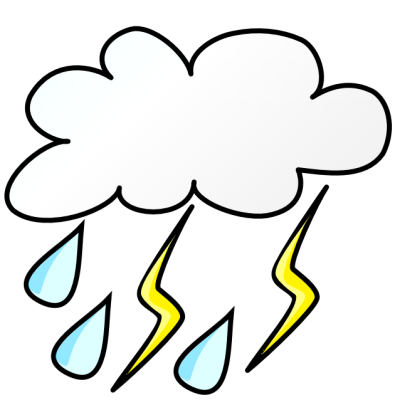
\includegraphics[width=0.2\textwidth]{./imagenes/tormenta.png} 
\caption{Nube de tormenta con rayos y lluvia}
\label{F:tormenta}
\end{figure}

La instrucción para insertar la gráfica es:


\begin{lstlisting}[]
\begin{figure}[H]
\centering
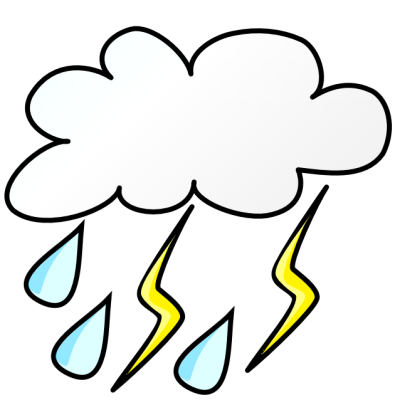
\includegraphics[width=0.2\textwidth]{./imagenes/tormenta.png} 
\caption{Nube de tormenta con rayos y lluvia}
\label{F:tormenta}
\end{figure}
\end{lstlisting}

La descripción es la siguiente:

\begin{itemize}\itemsep0pt \parskip0pt \parsep0pt
\item \verb+\begin{figure}[H]+ en la línea 1 inicia el entorno de la figura y declara que será ubicada inmediatamente luego del texto, con \verb+[H]+.
\item \verb+\centering+ en la línea 2 es una instrucción abreviada para indicar que la figura estará centrada.
\item \verb+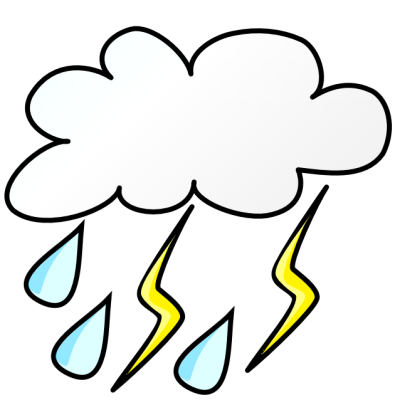
\includegraphics[width=0.2\textwidth]{./imagenes/tormenta.png}+ es la instrucción para insertar el archivo de la imagen, junto con indicaciones adicionales sobre el tamaño (un 20 \% del ancho del texto).
\item \verb+\caption{Nube de tormenta con rayos y lluvia}+ la instrucción  \texttt{caption}\footnote{En inglés, es bastante explícita esta instrucción, y en general puede decirse lo mismo de todos los comandos de \LaTeX, (ver por ejemplo \textsf{footnote}, \textsf{includegraphics}, \textsf{subsection}, etc.)} es el pie de figura con el nombre y la explicación. El número de figura lo inserta \LaTeX~ automáticamente.
\item \verb+\label{F:tormenta}+ es una etiqueta para referencia dentro de otras partes del texto.
\item \verb+\end{figure}+ cierra el entorno de la figura.
\end{itemize}

Como buena práctica, se recomienda nombrar el archivo de la imagen igual que la etiqueta, y con \textit{un nombre representativo}. Los nombres no deben tener espacios ni tildes ni eñes. Por ejemplo: \verb+senal_entrada_sinusoidal.jpg+.

\LaTeX, por defecto, va a ubicar las imágenes arriba o debajo de la página, y no inmediatamente después del texto en el que se escribe dentro del código, excepto que se indique lo contrario con \verb+\begin{figure}[h!]+ o con \verb+\begin{table}[H]+ utilizando el paquete \verb+float+.

Adicionalmente, se puede ubicar varias imágenes dentro de un mismo entorno de figura, como en la Figura \ref{F:subfiguras}. Ahí se muestran cuatro figuras distintas dentro del mismo entorno, donde se puede hacer referencia al transistor en \ref{F:subfig1}, al LED en \ref{F:subfig2}, al fotoconductor en \ref{F:subfig3} y al circuito integrado en \ref{F:subfig4}.

\begin{figure}[h!]
\centering
\subfloat[Transistor (texto que aparece en el índice)][Transistor en encapsulado TO-220]{
	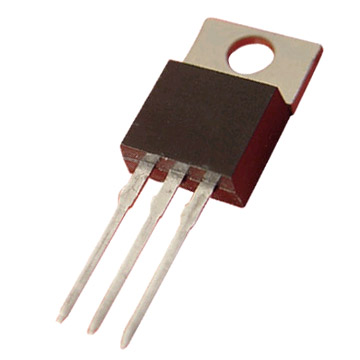
\includegraphics[width=0.2\textwidth]{./imagenes/transistor.jpg}
	\label{F:subfig1}}
\qquad
\subfloat[LED][LED blanco de baja potencia]{
	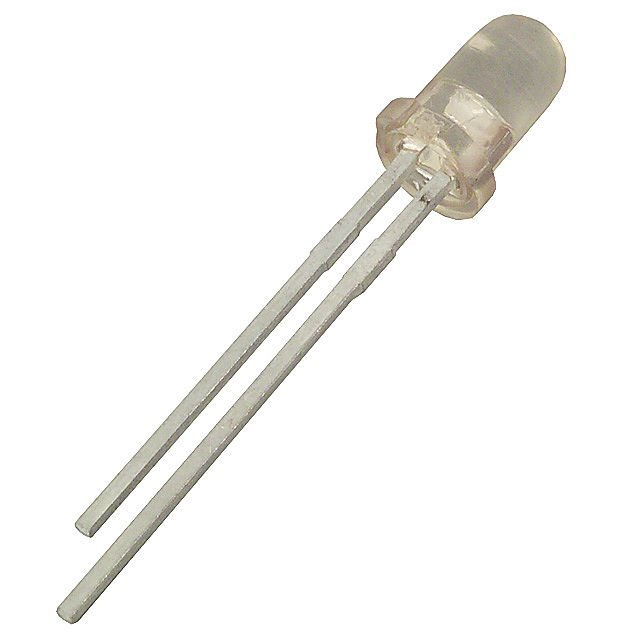
\includegraphics[width=0.2\textwidth]{./imagenes/led.jpg}
	\label{F:subfig2}}
\\
\subfloat[Fotoconductor][Fotoconductor]{
	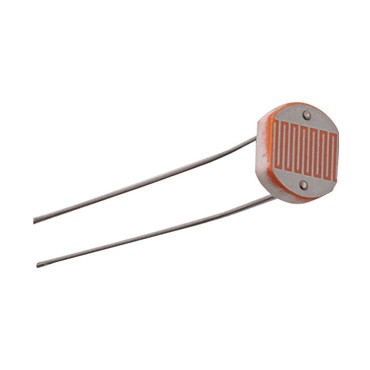
\includegraphics[width=0.2\textwidth]{./imagenes/fotoconductor.jpg}
	\label{F:subfig3}}
\qquad
\subfloat[Circuito integrado][Circuito integrado en encapsulado DIP-8]{
	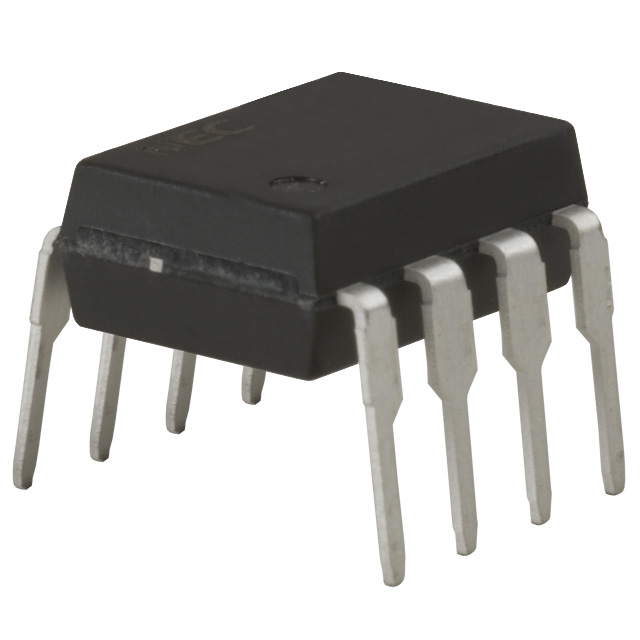
\includegraphics[width=0.2\textwidth]{./imagenes/integrado.jpg}
	\label{F:subfig4}}
\caption{Una figura con varias subfiguras, utilizando el paquete \texttt{subfig}}
\label{F:subfiguras}
\end{figure}

\subsection{Tablas}
%%%%%%%%%%%%%%%%%%%

Para las tablas se debe utilizar el entorno \verb+table+.

Aquí hay dos casos posibles:

\begin{description}

\item [Que la tabla debe construirse en \LaTeX] y en ese caso se debe usar el entorno \verb+tabular+, que a su vez se incluye dentro de \verb+table+.

\item [Que la tabla es en realidad una imagen] si fue generada por otro programa o fue escaneada, etc. Esta imagen entonces se incluye dentro del entorno \verb+table+ para que sea tratada como tal (y se numere como tabla, y se incluya en el índice de tablas, y se hagan las referencias como tablas, etc.).

\end{description}

Como ejemplo sencillo, la Tabla \ref{T:ejemplo} muestra una tabla con líneas verticales, declaradas como \verb+c | c+, que significa \textit{centrado - línea vertical - centrado}, y líneas horizontales, declaradas como \verb+\hline+ después de cada línea salto de línea (\verb+\\+).

\begin{table}
\caption{Comparación de velocidad de UWB con otros estándares alámbricos e inalámbricos}
\label{T:ejemplo}
\begin{center}
\begin{tabular}{ c | c}
\hline
\textbf{Velocidad [Mbits/s]} & \textbf{Estándar} \\ 
\hline
480 & UWB, USB 2.0 \\ 
200 & UWB (4 m) \\
110 & UWB (10 m) \\ 
90 & Fast Ethernet \\ 
54 & 802.11a \\ 
20 & 802.11g \\ 
11 & 802.11b \\ 
10 & Ethernet \\ 
3 & Bluetooth \\ 
0,256 & ZigBee \\ 
\hline
\end{tabular}
\end{center}
\end{table}

La instrucción \verb+\begin{tabular}{ | c | c |}+ genera un cuadro con líneas verticales en ambos lados, como en la Tabla \ref{T:ejemploconlineas}. 

Cuando se tiene un documento de dos o más columnas, es importante notar que una tabla puede ser muy grande y no quepa en una sola columna, por tanto debe especificarse que se acomode a todo lo ancho de la página. Esto es sencillo: basta con escribir \verb+table*+ al inicio y al final cuando se declara el entorno en \verb+\begin{} ... \end{}+.

\begin{table*}
\caption[Título en el índice]{Título que aparece en el pie de figura o encabezado de la tabla. Puede ser bastante amplio y explicar con más detalle. Debido a que el título que aparece en el índice es corto, no hay problema de que se exceda el espacio apropiado ahí.}
\label{T:ejemploconlineas}
\begin{center}
\begin{tabular}{| c | c |}
\hline
\textbf{Velocidad [Mbits/s]} & \textbf{Estándar} \\ 
\hline
480 & UWB, USB 2.0 \\ 
200 & UWB (4 m), 1394a (4,5 m) \\
110 & UWB (10 m) \\ 
90 & Fast Ethernet \\ 
54 & 802.11a \\ 
20 & 802.11g \\ 
11 & 802.11b \\ 
10 & Ethernet \\ 
3 & Bluetooth \\ 
0,256 & ZigBee \\ 
\hline
\end{tabular}
\end{center}
\end{table*}

Del mismo modo que en las figuras, \LaTeX~ por defecto colocará la tabla en la parte superior de la siguiente página, excepto que se indique lo contrario (con \verb+\begin{table}[h!]+)\footnote{Para mejor manejo de la posición de figuras, tablas y otros, utilizar el paquete \textsf{float}}.

\begin{table}
\caption{Otra tabla utilizando el paquete \texttt{booktabs}}
\label{T:otratabla}
\centering
\begin{tabular}{c l r r}
\toprule
\multicolumn{2}{c}{Producto} \\
\cmidrule(r){1-2}
Cantidad & Descripción & Precio unitario & Precio total  \\
\midrule
3  & Transistores 	& 250	& 750	\\
4  & Osciladores   	& 500   & 2000 \\
3  & Amp Ops     	& 600   & 1800	\\
10 & Resistores  	& 25    & 250	\\
10 & Capacitores	& 50 	& 500	\\
\midrule 
\multicolumn{3}{r}{TOTAL} & \textbf{5300} \\
\bottomrule
\end{tabular}
\end{table}

%%%%%%%%%%%%%%%%%%%%%%%%%%%%%
\section{Herramientas útiles}
%%%%%%%%%%%%%%%%%%%%%%%%%%%%%

%----------------------------------
\subsection{Referencias a figuras, tablas, ecuaciones, secciones y otros}

Es fundamental a lo largo del texto hacer referencias a figuras, tablas, ecuaciones, secciones y otros. Todos estos elementos tienen una etiqueta \verb+\label{}+ asociada a cada uno. 

La instrucción para hacer la referencia a esta etiqueta es \verb+\ref{}+.

Así entonces, se puede hacer referencia a las ecuaciones (\ref{E:desigualdad}), (\ref{E:anchodebanda}) y (\ref{E:fraccional}), a la Figura \ref{F:tormenta} y a la Tabla \ref{T:ejemplo} desde cualquier parte del texto, sin importar la numeración, que será asignada automáticamente por \LaTeX.

Es buena práctica nombrar las ecuaciones como \verb+\label{E:ecuacion}+, las tablas como \verb+\label{T:tabla}+, las figuras como \verb+\label{F:figura}+, y así sucesivamente, es decir, con una E, T, F o S antepuestas para identificar de qué se trata en cada caso, y con un nombre representativo. 

No es bueno hacer referencias relativas como ``la siguiente figura'' o ``la tabla anterior'' porque en realidad no se sabe la ubicación final dentro del texto. Hay que notar que tanto las tablas como las figuras, a menos de que se especifique lo contrario\footnote{Como se ha explicado, una forma de cambiar esto es colocando [h!] o [H] (de \emph{here}) junto al inicio del entorno.}, se colocarán al principio o al final de la página, en donde el programa lo considere mejor por motivo de espacio. Es mejor una referencia absoluta tal como figura \ref{F:tormenta} o ecuación (\ref{E:fraccional}). 

En editores de escritorio, algunas veces es necesario compilar dos o tres veces para que se carguen correctamente los números de referencia.

\subsection{Citas bibliográficas}
%%%%%%%%%%%%%%%%%%%%%%%%%%%%%%%%%
\label{S:citas_bibliograficas}

Los trabajos académicos requieren de referencias a las fuentes de información, invariablemente. Es necesario entonces considerar cómo crear una bibliografía y cómo referirse a las fuentes dentro del texto. 

Se puede hacer una bibliografía ``a mano'', en el que se le da la edición necesaria a cada entrada\footnote{En el código fuente de este documento hay un ejemplo de bibliografía tipo ``plain''.}. Sin embargo, BibTeX es una mejor alternativa, que permite administrar y modificar fácilmente una gran cantidad de entradas, además de que hace posible la reutilización de las referencias, en otros documentos.

\subsubsection{BibTeX}

\href{http://www.bibtex.org/}{BibTeX} es un programa de manejo de referencias. En este documento se utiliza de la siguiente forma:

\begin{itemize}
\item En un archivo llamado \texttt{bibliografia.bib} se introducen todas las referencias utilizadas, con el formato especial para ello. Ejemplo:
\begin{verbatim}
@BOOK {Valiente2001,
    author    = "Valiente Feruglio, G.",
    title     = "Composición de Textos Científicos con LaTeX",
    publisher = "Alfaomega",
    year      = "2001",
    address   = "México D.F.",
    edition   = "primera"
}
\end{verbatim}
Una buena herramienta para editar estas entradas se encuentra en \url{http://truben.no/latex/bibtex/}, sin embargo, considerar los sistemas de manejo bibliográfico de la siguiente sección.

\item Dentro del texto se hace referencia a las fuentes. La instrucción para hacer una cita es \verb+\cite{+\textit{clave}\verb+}+, dentro del cual se coloca la etiqueta, clave o \textit{key} asignada a la bibliografía (el primer espacio en la entrada de BibTeX de ejemplo), usualmente el apellido del primer autor y el año de publicación, por ejemplo: \verb+\cite{Valiente2001}+, que resulta en \cite{Valiente2001}.

\item Finalmente, al final del trabajo, se colocan las instrucciones 
\begin{verbatim}
\bibliographystyle{estilo}
\bibliography{nombrearchivo.bib}
\end{verbatim}
donde \texttt{estilo} es uno de los varios formatos posibles para las citas y las referencias (ver una lista en \url{https://www.sharelatex.com/learn/Bibtex_bibliography_styles}), y la segunda instrucción se encarga de colocar el título, y todas las entradas \textbf{que han sido citadas}, en el orden y el formato necesarios. Ahí es donde la ventaja de BibTeX se hace más evidente. 

\item En programas de edición de escritorio (Texmaker,\ldots) es necesario compilar varias veces y en una secuencia específica para que se genere la bibliografía. Esta secuencia es: \texttt{latex} \textgreater~ \texttt{bibtex} \textgreater~ \texttt{latex} \textgreater~ \texttt{latex}. En las plataformas de edición en línea (Overleaf,\ldots) esto se hace automáticamente.
\end{itemize}

\subsubsection{Sistemas de manejo bibliográfico}

En trabajos de investigación es necesario recurrir a muchas referencias (en tesis y otros, fácilmente más de 50) y el manejo de estas se puede tornar engorroso. Actualmente, varias plataformas ofrecen un manejo automatizado y muy conveniente de referencias. A continuación se presentan algunas opciones.

\begin{multicols}{2}
\begin{description}
\item[Mendeley] \url{http://www.mendeley.com/}
\item[Readcube] \url{http://www.readcube.com/}
\item[Docear] \url{http://www.docear.org/}
\item[Citavi] \url{http://www.citavi.com/}
\item[EndNote] \url{http://endnote.com/}
\item[JabRef] \url{http://jabref.sourceforge.net/}
\end{description}
\end{multicols}

\subsection{Formato}
%%%%%%%%%%%%%%%%%%%%

%---------------------------------------
\subsubsection{Cambiar el tipo de letra}

La tipografía de \LaTeX~ por defecto es la \href{https://en.wikipedia.org/wiki/Computer_Modern}{Computer Modern}. Es fácil de identificar y ampliamente utilizada (por la popularidad de \LaTeX) en muchas publicaciones científicas.

Esta plantilla de Proyecto Eléctrico utiliza la tipografía \href{http://www.linuxlibertine.org/}{Libertine}. 

Es útil, sin embargo, cambiar de tipografía en todo el documento o en algunas secciones\footnote{¡Cuidado! Demasiada libertad para cambiar el formato del documento puede derivar en malas decisiones de diseño gráfico. Ejemplo usual: utilizar Comic Sans (no disponible aquí).}.

Una referencia de la mayoría de tipografías disponibles para \LaTeX~ se encuentra en \url{http://www.tug.dk/FontCatalogue/}. Por ejemplo, la siguiente instrucción en el preámbulo convierte todo el texto a DejaVu Sans.

\begin{verbatim}
\usepackage{DejaVuSans}
\renewcommand*\familydefault{\sfdefault} 
\usepackage[T1]{fontenc}
\end{verbatim}

La instrucción \verb+{\fontfamily{qag}\selectfont ...texto...}+ genera {\fontfamily{qag}\selectfont un texto en otra tipografía. Para restringir la selección, el texto debe estar rodeado por llaves}. El código \texttt{qag} representa el tipo de letra. Una lista de tipos de letras y sus códigos, junto con más opciones se puede encontrar \href{https://www.sharelatex.com/learn/Font_typefaces}{aquí} y \href{http://tex.stackexchange.com/questions/25249/how-do-i-use-a-particular-font-for-a-small-section-of-text-in-my-document}{aquí}.

%-----------------------
\subsubsection{Unidades}

Las unidades deben escribirse separadas de la magnitud. Cuando se hace en una ecuación se presenta el problema que muestra la ecuación (\ref{E:sinunidades}). Para resolver este problema hay que incluir algún paquete que permita introducir unidades correctamente. En este documento se eligió \verb+siunitx+. La ecuación (\ref{E:conunidades}) muestra el uso corregido de las unidades en las ecuaciones. Del mismo modo, se puede poner de ejemplo: $C_s = \SI{0.1}{\micro\farad}$, $T_c = \SI{27}{\degreeCelsius}$. 

\begin{equation}\label{E:sinunidades}
{V}_{i}\ge 1,3 mV
\end{equation}

\begin{equation}\label{E:conunidades}
{V}_{i} \ge 1,3~\si{\milli\volt}
\end{equation}

O también el siguiente ejemplo:

\begin{equation}\label{E:unidades}
V = I_L \times R_L = \left( 0,25~\si{\milli\ampere} \right) \times \left( \SI{4}{\kilo\ohm} \right) = 1~\si{\volt} 
\end{equation}

%--------------------------------------------
\subsubsection{Otras herramientas de formato}

\begin{enumerate}
\item Las notas de pie\footnote{Que se insertan escribiendo la instrucción inmediatamente después del texto a comentar, como en este caso.}, utilizando la instrucción \verb+\footnote{}+.
\item Las comillas, que colocan con estos símbolos ``especiales'' y no las comillas del teclado. 
\item La palabra \LaTeX~ se escribe con el comando \verb+\LaTeX+. Debe escribirse el símbolo \verb+~+ después de la instrucción para que genere un espacio adecuado entre palabras, de otro modo \LaTeX queda pegado.
\item Las \textbf{negritas} se escriben con el comando \verb+\textbf{}+ (de \textit{\textbf{b}old \textbf{f}ace})
\item Las \textit{cursivas} se escriben con el comando \verb+\textit{}+ (de \textit{\textbf{it}alics})
\item Las \textsc{versales} se escriben con el comando \verb+\textsc{}+ (de \textit{\textbf{s}mall \textbf{c}aps})
\item Las \texttt{monoespacio} se escriben con el comando \verb+\texttt{}+ (de \textit{\textbf{t}ele\textbf{t}ype})
\item El comando \verb+\emph{}+ se utiliza para \emph{resaltar} un texto, muy similar a \verb+\textit{}+, con la diferencia que \textit{el resaltado depende del \emph{contexto} del párrafo}.
\item Hay varios tamaños de guiones: -, -- (con \verb+--+) y --- (con \verb+---+).
\item Se puede especificar la fecha de hoy, \today, utilizando el comando \verb+\today+.
\item El paquete \verb+hyperref+ permite la inclusión de hipervínculos, tanto a lugares externos del documento como internos (observe las referencias a tablas, figuras o ecuaciones o las citas bibliográficas). También incorpora los   marcadores que se muestran en los lectores de pdf y que se utilizan para navegación del documento. Por ejemplo, se puede hacer referencia a la Sección \ref{S:Figuras} donde se explica la inclusión de figuras (y hacer clic al hipervínculo y seguirlo).
\item Las listas numeradas (como esta) se hacen con el entorno \verb+\begin{enumerate}+, las listas con viñetas utilizando \verb+\begin{itemize}+.
\item Se pueden crear comandos especiales para insertar textos o símbolos definidos por el usuario. La instrucción es \verb+\newcommand{\comando}{Texto a introducir}+.
\item Por ejemplo, si no se quiere escribir cada vez ``Escuela de Ingeniería Eléctrica'' y además se le quiere dar un formato especial, entonces se puede indicar en el preámbulo 

\verb+\newcommand{\EIEx}{\textsc{Escuela \Lightning~ Ingeniería Eléctrica}}+ 

y así se crea el comando \verb+\EIEx+ que genera: \EIEx.
\item[--] Se puede utilizar un guión (o cualquier símbolo) en lugar de la numeración o las viñetas en una lista, con la instrucción \verb+[-]+ al lado de \verb+\item+.
\item[\Biohazard] Ejemplo de símbolo como viñeta\footnote{Las instrucciones \texttt{Lightning} y \texttt{Biohazard} son parte del paquete de símbolos especiales \texttt{marvosym}.}.
\end{enumerate}

\subsection{Figuras con PGF/Ti\textit{k}Z}
%%%%%%%%%%%%%%%%%%%%%%%%%%%%%%%%%%%%%%%%%%

PGF/Ti\textit{k}Z es un conjunto de lenguajes para producir gráficos vectoriales a partir de una descripción geométrica y algebraica\footnote{Tomado de su descripción en Wikipedia.}. Tiene grandes capacidades y una documentación exhaustiva.

La Figura \ref{F:tikz} es un ejemplo relativamente sencillo de las capacidades de Ti\textit{k}Z.

\begin{figure}[H]
\centering
	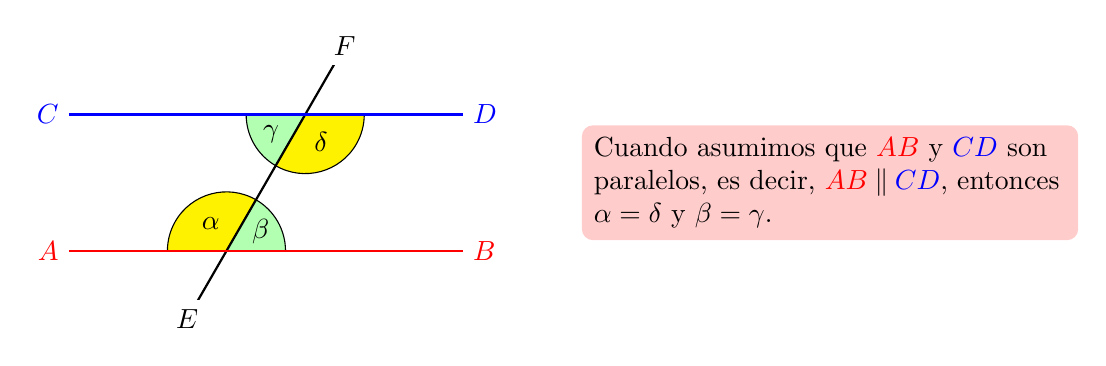
\begin{tikzpicture}
	  \draw[fill=yellow] (0,0) -- (60:.75cm) arc (60:180:.75cm);
	  \draw(120:0.4cm) node {$\alpha$};
	  \draw[fill=green!30] (0,0) -- (right:.75cm) arc (0:60:.75cm);
	  \draw(30:0.5cm) node {$\beta$};
	  \begin{scope}[shift={(60:2cm)}]
	    \draw[fill=green!30] (0,0) -- (180:.75cm) arc (180:240:.75cm);
	    \draw (30:-0.5cm) node {$\gamma$};
	    \draw[fill=yellow] (0,0) -- (240:.75cm) arc (240:360:.75cm);
	    \draw (-60:0.4cm) node {$\delta$};
	  \end{scope}
	  \begin{scope}[thick]
	    \draw  (60:-1cm) node[fill=white] {$E$} -- (60:3cm) node[fill=white] {$F$};
	    \draw[red]                   (-2,0) node[left] {$A$} -- (3,0) node[right]{$B$};
	    \draw[blue,shift={(60:2cm)}] (-3,0) node[left] {$C$} -- (2,0) node[right]{$D$};
	    \draw[shift={(60:1cm)},xshift=4cm]
	    node [right,text width=6cm,rounded corners,fill=red!20,inner sep=1ex]
	    {
	      Cuando asumimos que $\color{red}AB$ y $\color{blue}CD$ son paralelos, es decir, ${\color{red}AB} \mathbin{\|} \color{blue}CD$, entonces $\alpha = \delta$ y $\beta = \gamma$.
	    };
	  \end{scope}
	\end{tikzpicture}
\caption[Ejemplo de uso de PGF/Ti\textit{k}Z]{Ejemplo de uso de PGF/Ti\textit{k}Z, pero solo una muestra de sus capacidades.}
\label{F:tikz}
\end{figure}

Una buena cantidad de ejemplos están disponibles en \url{http://www.texample.net/tikz/} y la documentación (incluyendo un manual de uso de más de 700 páginas) está en \url{https://www.ctan.org/pkg/pgf?lang=en}.

%---------------------------------------
\subsection{Gráfico de datos y funciones con \texttt{pgfplots}}

%---------------------------------------
\subsection{Circuitos con Circuitikz}

El paquete \texttt{circuitikz} permite la creación de circuitos eléctricos y electrónicos. La Figura \ref{F:ampop} es un ejemplo.

\begin{figure}
  	\centering
		 \begin{circuitikz}[american]
		  \draw
		  % El amplificador operacional
		  (0,0) node[op amp] (opamp) {} node[] {{\tiny Amp Op}}
		  
		  % Las entradas
		  (opamp.-) node[circ] {} to[R, l_=$R_1$] ++(-2,0) node[ocirc] {} node[left] {$V_{s}$}
		  (opamp.+) -- ++(0,-0.5) node[ground] {} 
		  
		  % El lazo de realimentación
		  (opamp.-) -- ++(0,1)  to[R, l=$R_2$] ++(2,0) -| (opamp.out) {}
		  
		  % La salida
		  (opamp.out) -- ++(0.5,0) node[circ] {} to[R, l=$R_L$] ++(0,-2) to [short, i_=$I_o$] ++(0,0) node[ground] {}
		  (opamp.out) -- ++(1,0) node[ocirc] {} node[right]{$V_o$}
		  
		  ;
		\end{circuitikz}
    \caption[Amplificador inversor]{Amplificador inversor con un amplificador operacional cuya relación entrada--salida está dada por $V_o = -\frac{R_2}{R_1} V_s$.}
    \label{F:ampop}
\end{figure}

\begin{figure}
\centering
\input{imagenes/circuitobasico.tikz}
\caption{Circuito básico.}
\label{F:circuitobasico}
\end{figure}

\begin{figure}
\centering
\input{imagenes/transmisionpotencia.tikz}
\caption[Circuito de transmisión de potencia]{Circuito de transmisión de potencia por varias líneas conductoras desde centros de generación y con sistemas de ajuste de la corriente.}
\label{F:transmisionpotencia}
\end{figure}

\begin{figure}
\centering
\input{imagenes/acondicionamiento.tikz}
\caption[Circuito de acondicionamiento y amplificación]{Circuito de acondicionamiento y amplificación de la señal de un sensor resistivo $R_T$, dependiente de la temperatura.}
\label{F:acondicionamiento}
\end{figure}

\begin{figure}
\centering
\input{imagenes/reguladorlineal.tikz}
\caption{Regulador lineal de tensión con lazo de control.}
\label{F:reguladorlineal}
\end{figure}

\begin{figure}
\centering
\input{imagenes/protecciontermica.tikz}
\caption{Circuito para protección térmica con lazo de histéresis.}
\label{F:protecciontermica}
\end{figure}

\subsection{Inserción de código fuente}
%%%%%%%%%%%%%%%%%%%%%%%%%%%%%%%%%%%%%%%

En ocasiones es necesario introducir secciones de código fuente de programación dentro de reportes. La inserción es especial, pues el compilador no debe confundir las instrucciones dentro del código con instrucciones de \LaTeX. Además, se prefiere un formato específico con resaltado de sintaxis para mejorar la legibilidad (como en los editores de código o en los IDE). Un paquete que provee soluciones para este requisito es \texttt{listings}.

Para el código fuente hecho en Matlab es posible utilizar el paquete \texttt{mcode} (adjunto como archivo a la carpeta que contiene el proyecto) que asigna a \texttt{listings} el formato apropiado, como se ve en el siguiente código:

\lstinputlisting[inputencoding=latin1]{codigo/codigoejemplo.m}

%%%%%%%%%%%%%%%%%%%%%%%%%%%%%%%%%
\section{Referencias para \LaTeX}
%%%%%%%%%%%%%%%%%%%%%%%%%%%%%%%%%

La comunidad de usuarios de \LaTeX~ es grande y colaborativa. Hay multitud de recursos en línea para aprender buenas prácticas y ``trucos'' para mejorar los documentos. Algunas de las mejores referencias son:

\begin{description}
\item[Wikibook] \url{https://en.wikibooks.org/wiki/LaTeX}
\item[Cookbook] \url{http://latex-cookbook.net/}
\item[TeXample] \url{http://texample.net/}
\item[HowtoTeX] \url{http://www.howtotex.com/}
\item[Font Catalogue] \url{http://www.tug.dk/FontCatalogue/}
\end{description}

\subsection{¿Dónde editar \LaTeX?}\label{S:programas}
%%%%%%%%%%%%%%%%%%%%%%%%%%%%%%%%%%%%%%%%%%%

\paragraph{Editores de texto ``de escritorio''}

Existen varios programas para la edición y compilación de archivos de \LaTeX. Se ha escogido Texmaker debido a que es multiplataforma (Mac, Linux, Windows) y cuenta con otras características como resaltado de sintaxis, autocompletar, corrección ortográfica, asistente para la creación de documentos, accesos rápidos a símbolos, comandos y entornos, entre otros. Se puede, claro está, editar el documento con cualquier editor y compilar, siempre y cuando se tengan los paquetes necesarios\footnote{Esta es una ventaja de ser un código estándar abierto.}.

En Windows, junto con Texmaker debe instalarse MiKTeX, que es un conjunto de paquetes, fuentes y demás necesarios para compilar el archivo.

Ambos están disponibles para descarga gratuita desde \url{http://miktex.org/} y \url{http://www.xm1math.net/texmaker/}.

Una base de datos extensiva de los paquetes de \LaTeX~ está en \url{http://www.ctan.org/}. Es especialmente útil para encontrar la documentación de los paquetes. Desde esta página se pueden descargar los paquetes, pero la mejor forma de revisar los paquetes disponibles e instalarlos fácilmente es a través del \emph{MiKTeX Package Manager}, disponible después de instalar el MiKTeX.

\paragraph{Plataformas en línea de edición para \LaTeX}

Una alternativa muy popular de años muy recientes es la edición en línea. Entre las ventajas se encuentran: almacenamiento en línea, edición colaborativa, herramientas web (bibliografías y otros), compilación simultánea, más la mayoría de las otras ventajas de los editores ``de escritorio'' como autocompletar, símbolos, etc.

Los editores más populares son:

\begin{description}
\item[Overleaf] \url{https://www.overleaf.com/}
\item[ShareLaTeX] \url{https://www.sharelatex.com/}
\item[Papeeria] \url{https://papeeria.com/}
\end{description}
% ----------------------------------------
  \chapter{Conclusiones y recomendaciones}
% ----------------------------------------
\label{C:conclusiones}

El informe debe terminarse con la enumeración de las principales conclusiones derivados del trabajo realizado.  En particular, debe verificarse el cumplimiento de los objetivos planteados para el mismo.

\section{Conclusiones}
El aporte (\emph{novedad}) hecho con el proyecto, debe destacarse.

Las conclusiones pueden enumerarse en forma suscinta como una lista, ya sea itemizada o numerada.

\section{Recomendaciones}
Con base en las trabajo realizado y las conclusiones sobre el mismo, puede ser necesario incluir una sección, o lista, de recomendaciones.  Por ejemplo, sobre la utilización de otro enfoque para resolver el problema.

% 8. APÉNDICES
\appendix
\chapter{Apéndice de ejemplo}

\lipsum[3]

\section{Una sección del apéndice}

\lipsum[4]

\subsection{Y una sub-sección}

\lipsum[5-8]

\subsection{Y otra sub-sección}

\lipsum[5-8]
\chapter{Un apéndice ejemplo con archivo anexo}

Para insertar archivos \texttt{.pdf} se utiliza el paquete \texttt{pdfpages}. Este paquete tiene opciones disponibles para la configuración del documento inserto.

Aquí hay dos ejemplos sencillos.

%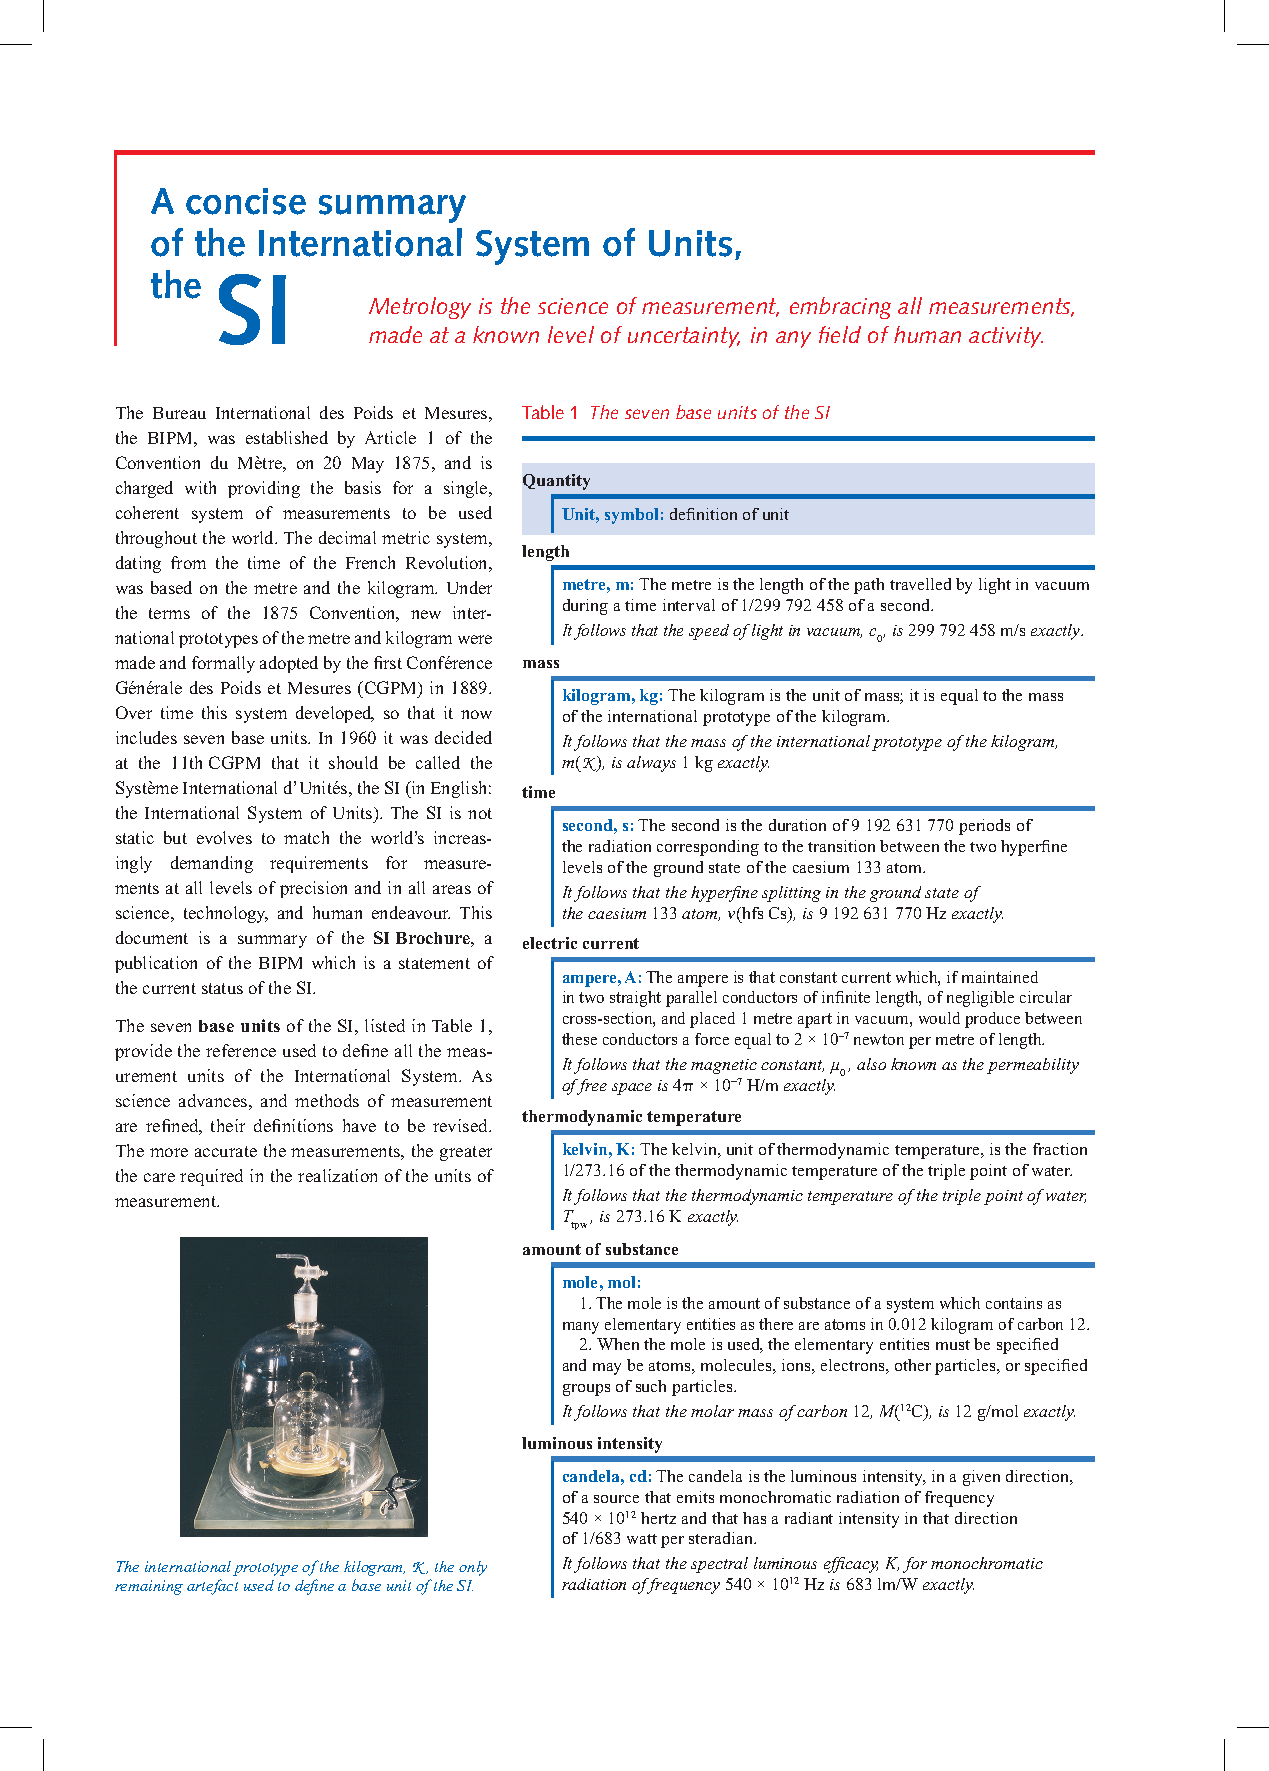
\includepdf[pages=-,nup=2x2]{apendices/SIsummary.pdf}

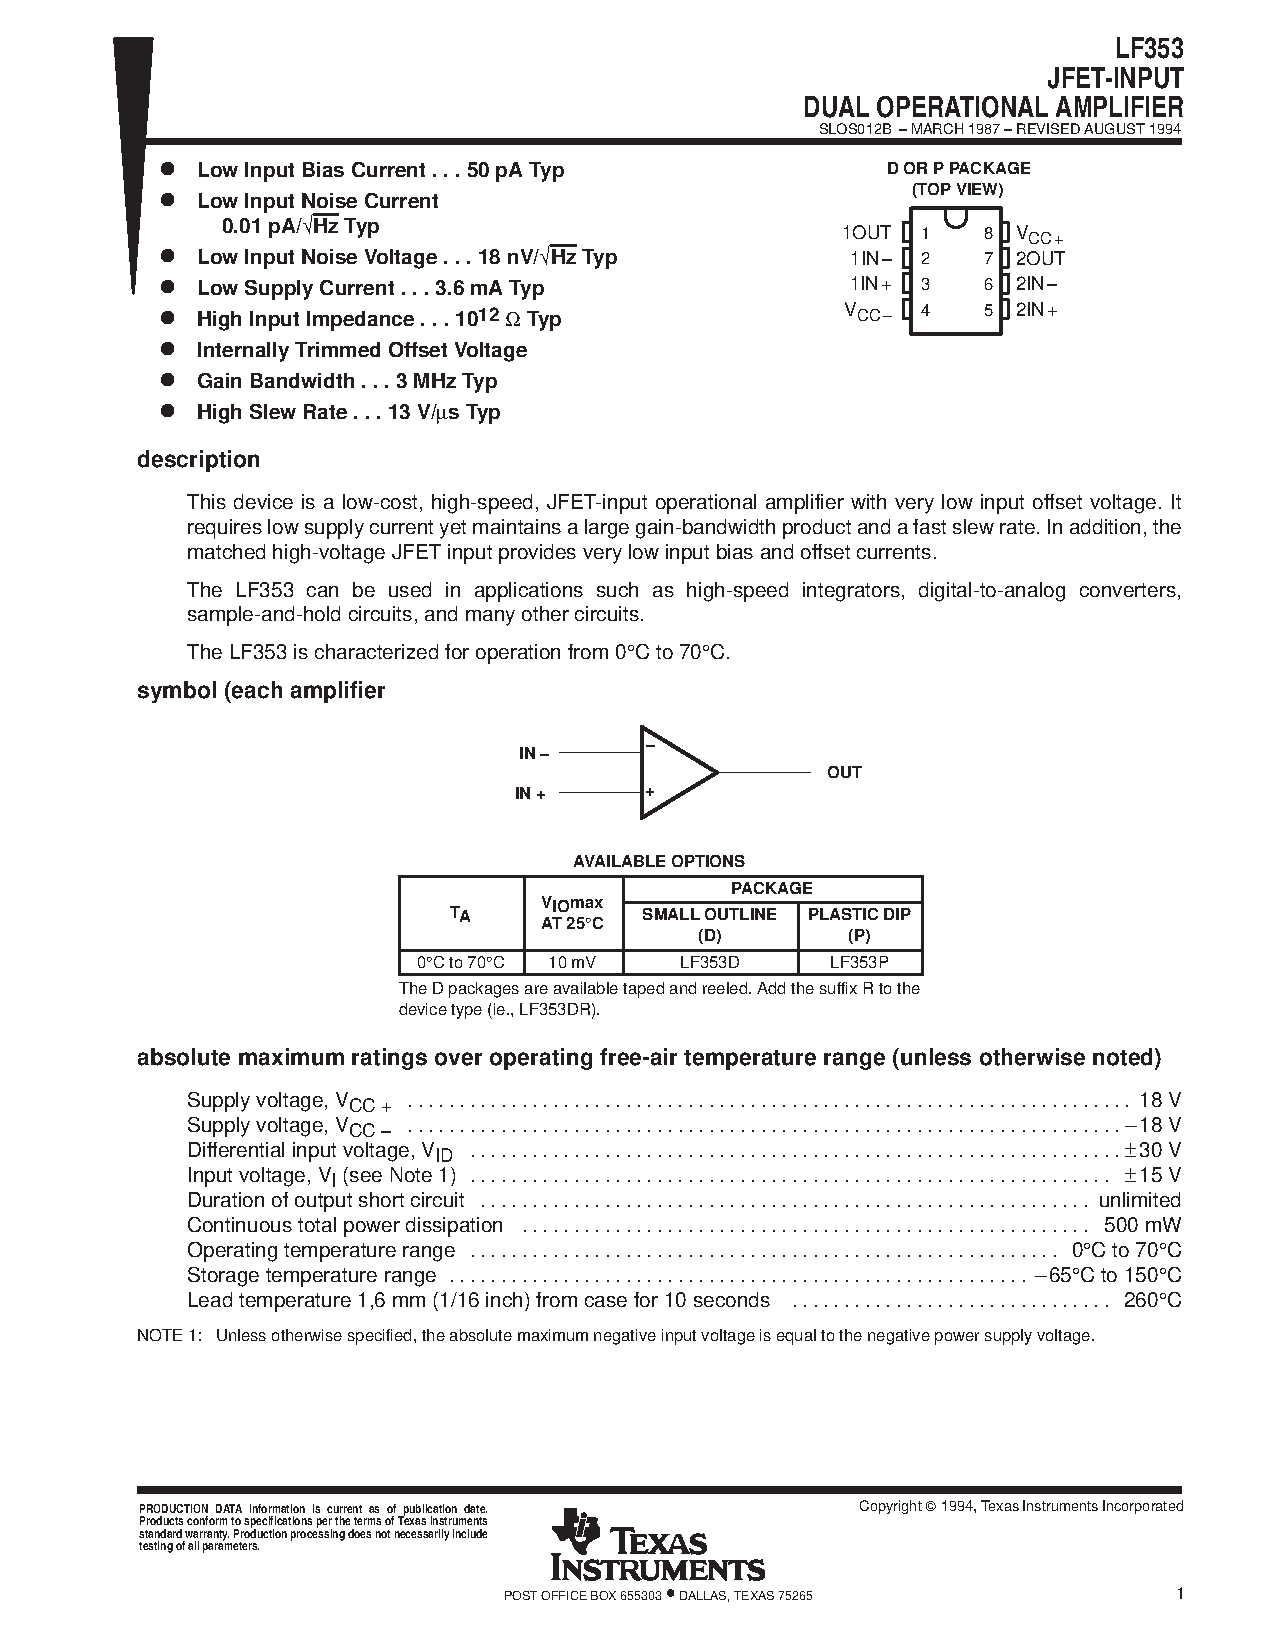
\includepdf[pages=1]{apendices/LF353.pdf}

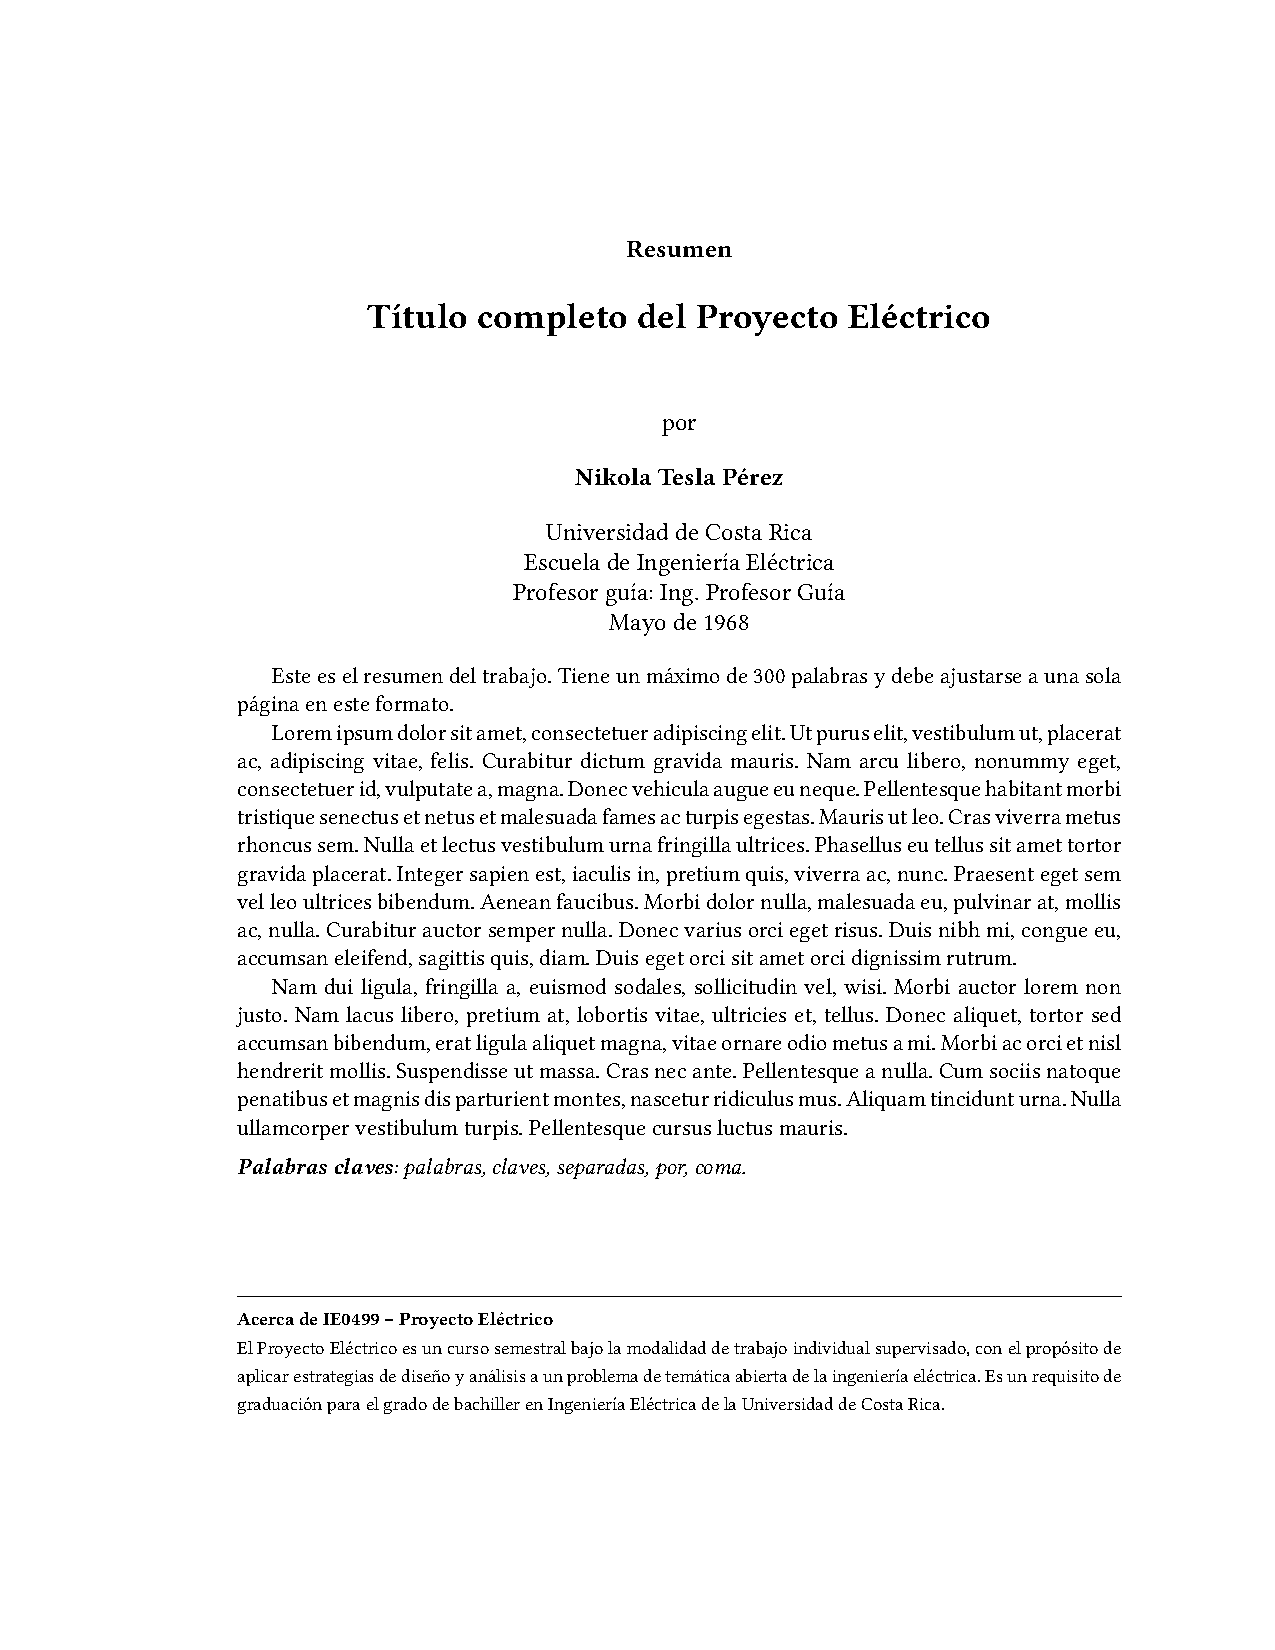
\includepdf[pages=-,scale=0.6,pagecommand={}]{apendices/Resumen.pdf}

\backmatter

% 9. BILIOGRAFÍA
\bibliographystyle{plain}
\bibliography{bibliografia/bibliografia.bib}

%%%%%%%%%%%%%%%%%%%
\end{document}
%%%%%%%%%%%%%%%%%%%
\end{verbatim}

%%%%%%%%%%%%%%%%%%%%%%%%%%%%%%%%%%%%%%%%%%%%%%
\section{Las partes de un documento de \LaTeX}
%%%%%%%%%%%%%%%%%%%%%%%%%%%%%%%%%%%%%%%%%%%%%%

\subsection{Preámbulo y cuerpo del documento}
%%%%%%%%%%%%%%%%%%%%%%%%%%%%%%%%%%%%%%%%%%%%%

Los archivos \texttt{.tex} de donde se generan los documentos en \LaTeX~ tienen dos grandes secciones: el encabezado o preámbulo y el cuerpo del documento.

En el \textbf{encabezado} del documento se definen los parámetros más importantes del documento, y se invocan los ``paquetes'' que permiten la edición de características especiales. Entre las características que se pueden definir aquí están: tamaño del papel, tamaño y tipo de tipografía, tipo de documento (reporte, artículo, libro, carta\ldots), numeración, autor, fecha, título y más. 

Además de estas definiciones generales, se deben cargar todos los \textbf{paquetes} que permiten hacer ediciones especiales como: introducir hipervínculos, agregar colores, agregar imágenes, editar encabezados y pies de página, etc. 

Para utilizar un paquete se escribe la instrucción \verb+\usepackage[opciones]{nombredelpaquete}+, donde las opciones están definidas por cada paquete particular. 

Por ejemplo \verb+\usepackage[spanish]{babel}+. El paquete Babel permite cambiar la lengua del documento (en inglés por defecto), y entre paréntesis cuadrado se especifica que sea español.

Los paquetes que utiliza \LaTeX~ están en un repositorio (ver Sección \ref{S:programas}). La documentación de los paquetes puede encontrarse en la página de CTAN (\textit{Comprehensive TEX Archive Network}), \url{https://www.ctan.org/}.

Uno de los elementos más importantes de \LaTeX~ es el \emph{entorno}. Un entorno (\emph{environment}) siempre inicia con \verb+\begin{nombredelentorno}+ y finaliza con \verb+\end{nombredelentorno}+. Dentro de él, todo el contenido va a tener un formato característico dependiendo del tipo de entorno. Las ecuaciones, figuras y tablas tienen su propio entorno. Hay otros para listas numeradas, resumen, teoremas, texto centrado\ y más. El mismo cuerpo del documento es un gran entorno \texttt{document}.

A continuación se describirá el uso de algunos de los entornos más importantes: ecuaciones, tablas y figuras.

\subsection{Ecuaciones}
%%%%%%%%%%%%%%%%%%%%%%%

Hay tres tipos de ecuaciones posibles: unas en línea, o dentro del párrafo, otras en modo \emph{display} con numeración y sin numeración. 

\begin{description}

\item [Las ecuaciones en línea] están rodeadas por los símbolos \verb+$ $+ (una forma abreviada de crear el entorno). Se utilizan cuando se coloca una fórmula en un párrafo, por ejemplo $ {{B}_{f}}\ge 0,2 $, que no lleva numeración y que debe estar alineada con el texto. \LaTeX~ se encargará de ajustar su tamaño y ubicación, como cuando se introduce una raíz cuadrada $ \sqrt {{b^2} - 4ac} $ o una integral  $ \int_0^\infty e^{-x}\,\mathrm{d}x $. 

\item [Las ecuaciones numeradas] se hacen dentro del entorno \texttt{equation}. Ejemplos de ecuaciones se muestran a continuación.

\begin{verbatim}
\begin{equation}
x_{1,2} = \frac{-b \pm \sqrt{b^2 - 4ac}}{2a}
\end{equation}
\end{verbatim}

\begin{equation}
x_{1,2} = \frac{-b \pm \sqrt{b^2 - 4ac}}{2a}
\end{equation}

\begin{equation}\label{E:desigualdad}
{B}_{f}\ge 0,2
\end{equation}

\begin{equation}\label{E:anchodebanda}
BW\ge 500\text{ MHz}
\end{equation}

donde $ {B}_{f} $ es el ancho de banda fraccional y se define como:

\begin{equation}\label{E:fraccional}
{{B}_{f}}=\frac{BW}{{{f}_{c}}}=\frac{\left( {{f}_{H}}-{{f}_{L}} \right)}{{\left( {{f}_{H}}+{{f}_{L}} \right)}/{2}\;}
\end{equation}

donde $f_H$ y $f_L$ son las frecuencias superior e inferior de la banda de transmisión de -10 dB, $ BW $ es el ancho de banda y $f_c$ la frecuencia central.

El estilo de la numeración depende del tipo de documento (\texttt{article}, \texttt{report}, \texttt{book}\ldots) y obedecerá (si no se especifica lo contrario) la secuencia numérica.

\item [La ecuaciones no numeradas] se deben utilizar en ocasiones, sobre todo cuando se trata de pasos intermedios o cálculos y no la deducción de alguna expresión. Para ello se deben utilizar los símbolos \verb+\[+ y \verb+\]+ (otra forma abreviada de crear el entorno) para rodear la ecuación.

\[
 \lim_{x \to \infty} \exp(-x) = 0
\]

\[
 R_{pu} = 2,7~\si{\kilo\ohm}
\]

\end{description}

Será necesario también en ocasiones incluir texto dentro de las ecuaciones. Pero es necesario escribir este texto dentro de los comandos \verb+\text{}+, \verb+\textbf{}+ o similares, para que se les aplique el espaciado y formato correctos. De otro modo sucede lo que se muestra en la ecuación (\ref{E:sintexto}), mientras que la ecuación (\ref{E:contexto}) muestra el uso corregido, incluyendo cierto formato añadido para resaltar.

\begin{equation}\label{E:sintexto}
Ciclo de trabajo = \frac{Tiempo en alto}{Per\acute{i}odo}
\end{equation}

\begin{equation}\label{E:contexto}
\text{Ciclo de trabajo} = \frac{\textsf{Tiempo en alto}}{\textbf{Per\'{i}odo}}
\end{equation}

A pesar de que la escritura de ecuaciones directamente en \LaTeX~ puede resultar algo complicada al principio, basta con una rápida investigación en la vasta información de las referencias suministradas y en la red\footnote{Hay muchas comunidades de usuarios en internet en foros y demás que resuelven estos problemas típicos} para encontrar la forma de realizar la ecuación deseada. Como alternativa, se puede utilizar un editor gráfico de ecuaciones como \href{http://www.dessci.com/en/products/mathtype/}{MathType} y de ahí exportar a \LaTeX\footnote{Para hacerlo: en la ventana de edición de ecuaciones de MathType se debe ir a \textsf{Preferences / Cut and Copy Preferences}, en la ventana emergente se debe seleccionar la opción \textsf{MathML or TeX} y en la lista desplegable escoger \textsf{LaTeX 2.09 and later}. En la misma ventana de edición se selecciona y copia la ecuación. La barra de estado mostrará: \textsf{Translated (LaTeX 2.09 and later)}.}. Es necesario, aún así, aprender los comandos básicos que facilitan y hacen más rápida la composición de fórmulas.

También se pueden editar ecuaciones en la aplicación en internet disponible en \url{http://rinconmatematico.com/latexrender/} en la cual se puede ver el resultado de la ecuación editada.

\subsection{Figuras}\label{S:Figuras}
%%%%%%%%%%%%%%%%%%%%%%%%%%%%%%%%%%%%%

Para las figuras existe un entorno llamado \verb+figure+, dentro del cual se ubican y configuran las imágenes.

Para ``llamar'' al archivo se debe hacer una referencia a su ubicación. Si está ubicada en la misma carpeta del documento se escribe \verb+nombre_de_la_imagen.jpg+\footnote{O cualquier formato de imágenes soportado, como .png, .gif y otros}. Pero los archivos de imágenes, de preferencia y por una cuestión de orden, deben colocarse dentro de una carpeta dedicada. Entonces, si está dentro de una carpeta se indica \verb+./carpeta/nombre_de_la_imagen.jpg+. Para subir un nivel en las carpetas se utiliza \verb+../carpeta/subcarpeta/nombre_de_la_imagen.jpg+. 

La imagen ``Nube de tormenta con rayos y lluvia'' es un ejemplo de imagen insertada.

\begin{figure}[H]
\centering
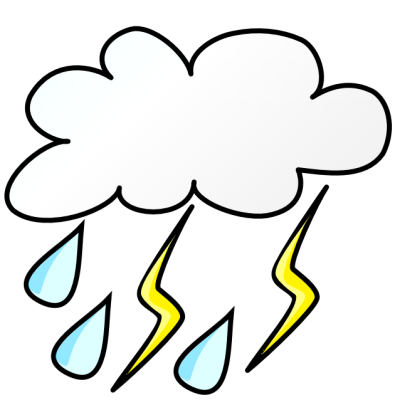
\includegraphics[width=0.2\textwidth]{./imagenes/tormenta.png} 
\caption{Nube de tormenta con rayos y lluvia}
\label{F:tormenta}
\end{figure}

La instrucción para insertar la gráfica es:


\begin{lstlisting}[]
\begin{figure}[H]
\centering
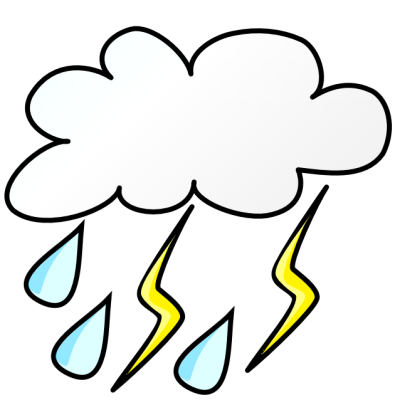
\includegraphics[width=0.2\textwidth]{./imagenes/tormenta.png} 
\caption{Nube de tormenta con rayos y lluvia}
\label{F:tormenta}
\end{figure}
\end{lstlisting}

La descripción es la siguiente:

\begin{itemize}\itemsep0pt \parskip0pt \parsep0pt
\item \verb+\begin{figure}[H]+ en la línea 1 inicia el entorno de la figura y declara que será ubicada inmediatamente luego del texto, con \verb+[H]+.
\item \verb+\centering+ en la línea 2 es una instrucción abreviada para indicar que la figura estará centrada.
\item \verb+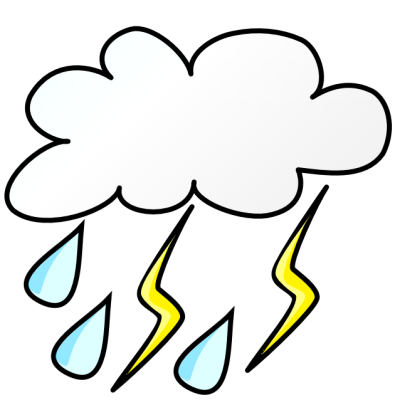
\includegraphics[width=0.2\textwidth]{./imagenes/tormenta.png}+ es la instrucción para insertar el archivo de la imagen, junto con indicaciones adicionales sobre el tamaño (un 20 \% del ancho del texto).
\item \verb+\caption{Nube de tormenta con rayos y lluvia}+ la instrucción  \texttt{caption}\footnote{En inglés, es bastante explícita esta instrucción, y en general puede decirse lo mismo de todos los comandos de \LaTeX, (ver por ejemplo \textsf{footnote}, \textsf{includegraphics}, \textsf{subsection}, etc.)} es el pie de figura con el nombre y la explicación. El número de figura lo inserta \LaTeX~ automáticamente.
\item \verb+\label{F:tormenta}+ es una etiqueta para referencia dentro de otras partes del texto.
\item \verb+\end{figure}+ cierra el entorno de la figura.
\end{itemize}

Como buena práctica, se recomienda nombrar el archivo de la imagen igual que la etiqueta, y con \textit{un nombre representativo}. Los nombres no deben tener espacios ni tildes ni eñes. Por ejemplo: \verb+senal_entrada_sinusoidal.jpg+.

\LaTeX, por defecto, va a ubicar las imágenes arriba o debajo de la página, y no inmediatamente después del texto en el que se escribe dentro del código, excepto que se indique lo contrario con \verb+\begin{figure}[h!]+ o con \verb+\begin{table}[H]+ utilizando el paquete \verb+float+.

Adicionalmente, se puede ubicar varias imágenes dentro de un mismo entorno de figura, como en la Figura \ref{F:subfiguras}. Ahí se muestran cuatro figuras distintas dentro del mismo entorno, donde se puede hacer referencia al transistor en \ref{F:subfig1}, al LED en \ref{F:subfig2}, al fotoconductor en \ref{F:subfig3} y al circuito integrado en \ref{F:subfig4}.

\begin{figure}[h!]
\centering
\subfloat[Transistor (texto que aparece en el índice)][Transistor en encapsulado TO-220]{
	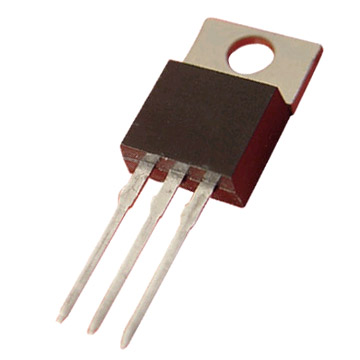
\includegraphics[width=0.2\textwidth]{./imagenes/transistor.jpg}
	\label{F:subfig1}}
\qquad
\subfloat[LED][LED blanco de baja potencia]{
	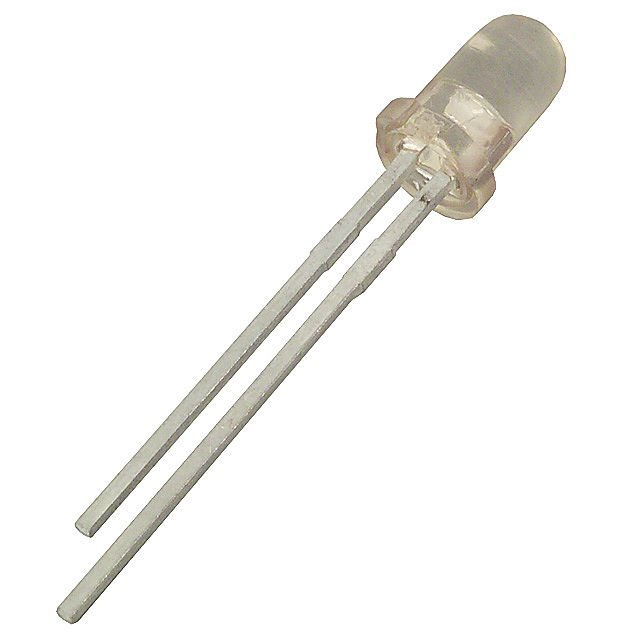
\includegraphics[width=0.2\textwidth]{./imagenes/led.jpg}
	\label{F:subfig2}}
\\
\subfloat[Fotoconductor][Fotoconductor]{
	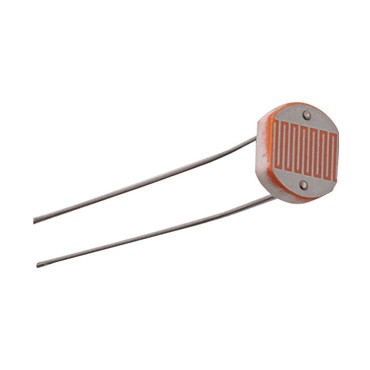
\includegraphics[width=0.2\textwidth]{./imagenes/fotoconductor.jpg}
	\label{F:subfig3}}
\qquad
\subfloat[Circuito integrado][Circuito integrado en encapsulado DIP-8]{
	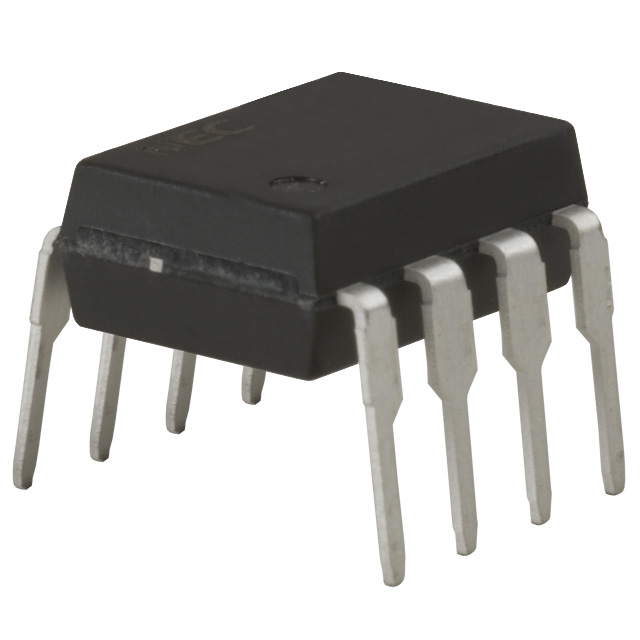
\includegraphics[width=0.2\textwidth]{./imagenes/integrado.jpg}
	\label{F:subfig4}}
\caption{Una figura con varias subfiguras, utilizando el paquete \texttt{subfig}}
\label{F:subfiguras}
\end{figure}

\subsection{Tablas}
%%%%%%%%%%%%%%%%%%%

Para las tablas se debe utilizar el entorno \verb+table+.

Aquí hay dos casos posibles:

\begin{description}

\item [Que la tabla debe construirse en \LaTeX] y en ese caso se debe usar el entorno \verb+tabular+, que a su vez se incluye dentro de \verb+table+.

\item [Que la tabla es en realidad una imagen] si fue generada por otro programa o fue escaneada, etc. Esta imagen entonces se incluye dentro del entorno \verb+table+ para que sea tratada como tal (y se numere como tabla, y se incluya en el índice de tablas, y se hagan las referencias como tablas, etc.).

\end{description}

Como ejemplo sencillo, la Tabla \ref{T:ejemplo} muestra una tabla con líneas verticales, declaradas como \verb+c | c+, que significa \textit{centrado - línea vertical - centrado}, y líneas horizontales, declaradas como \verb+\hline+ después de cada línea salto de línea (\verb+\\+).

\begin{table}
\caption{Comparación de velocidad de UWB con otros estándares alámbricos e inalámbricos}
\label{T:ejemplo}
\begin{center}
\begin{tabular}{ c | c}
\hline
\textbf{Velocidad [Mbits/s]} & \textbf{Estándar} \\ 
\hline
480 & UWB, USB 2.0 \\ 
200 & UWB (4 m) \\
110 & UWB (10 m) \\ 
90 & Fast Ethernet \\ 
54 & 802.11a \\ 
20 & 802.11g \\ 
11 & 802.11b \\ 
10 & Ethernet \\ 
3 & Bluetooth \\ 
0,256 & ZigBee \\ 
\hline
\end{tabular}
\end{center}
\end{table}

La instrucción \verb+\begin{tabular}{ | c | c |}+ genera un cuadro con líneas verticales en ambos lados, como en la Tabla \ref{T:ejemploconlineas}. 

Cuando se tiene un documento de dos o más columnas, es importante notar que una tabla puede ser muy grande y no quepa en una sola columna, por tanto debe especificarse que se acomode a todo lo ancho de la página. Esto es sencillo: basta con escribir \verb+table*+ al inicio y al final cuando se declara el entorno en \verb+\begin{} ... \end{}+.

\begin{table*}
\caption[Título en el índice]{Título que aparece en el pie de figura o encabezado de la tabla. Puede ser bastante amplio y explicar con más detalle. Debido a que el título que aparece en el índice es corto, no hay problema de que se exceda el espacio apropiado ahí.}
\label{T:ejemploconlineas}
\begin{center}
\begin{tabular}{| c | c |}
\hline
\textbf{Velocidad [Mbits/s]} & \textbf{Estándar} \\ 
\hline
480 & UWB, USB 2.0 \\ 
200 & UWB (4 m), 1394a (4,5 m) \\
110 & UWB (10 m) \\ 
90 & Fast Ethernet \\ 
54 & 802.11a \\ 
20 & 802.11g \\ 
11 & 802.11b \\ 
10 & Ethernet \\ 
3 & Bluetooth \\ 
0,256 & ZigBee \\ 
\hline
\end{tabular}
\end{center}
\end{table*}

Del mismo modo que en las figuras, \LaTeX~ por defecto colocará la tabla en la parte superior de la siguiente página, excepto que se indique lo contrario (con \verb+\begin{table}[h!]+)\footnote{Para mejor manejo de la posición de figuras, tablas y otros, utilizar el paquete \textsf{float}}.

\begin{table}
\caption{Otra tabla utilizando el paquete \texttt{booktabs}}
\label{T:otratabla}
\centering
\begin{tabular}{c l r r}
\toprule
\multicolumn{2}{c}{Producto} \\
\cmidrule(r){1-2}
Cantidad & Descripción & Precio unitario & Precio total  \\
\midrule
3  & Transistores 	& 250	& 750	\\
4  & Osciladores   	& 500   & 2000 \\
3  & Amp Ops     	& 600   & 1800	\\
10 & Resistores  	& 25    & 250	\\
10 & Capacitores	& 50 	& 500	\\
\midrule 
\multicolumn{3}{r}{TOTAL} & \textbf{5300} \\
\bottomrule
\end{tabular}
\end{table}

%%%%%%%%%%%%%%%%%%%%%%%%%%%%%
\section{Herramientas útiles}
%%%%%%%%%%%%%%%%%%%%%%%%%%%%%

%----------------------------------
\subsection{Referencias a figuras, tablas, ecuaciones, secciones y otros}

Es fundamental a lo largo del texto hacer referencias a figuras, tablas, ecuaciones, secciones y otros. Todos estos elementos tienen una etiqueta \verb+\label{}+ asociada a cada uno. 

La instrucción para hacer la referencia a esta etiqueta es \verb+\ref{}+.

Así entonces, se puede hacer referencia a las ecuaciones (\ref{E:desigualdad}), (\ref{E:anchodebanda}) y (\ref{E:fraccional}), a la Figura \ref{F:tormenta} y a la Tabla \ref{T:ejemplo} desde cualquier parte del texto, sin importar la numeración, que será asignada automáticamente por \LaTeX.

Es buena práctica nombrar las ecuaciones como \verb+\label{E:ecuacion}+, las tablas como \verb+\label{T:tabla}+, las figuras como \verb+\label{F:figura}+, y así sucesivamente, es decir, con una E, T, F o S antepuestas para identificar de qué se trata en cada caso, y con un nombre representativo. 

No es bueno hacer referencias relativas como ``la siguiente figura'' o ``la tabla anterior'' porque en realidad no se sabe la ubicación final dentro del texto. Hay que notar que tanto las tablas como las figuras, a menos de que se especifique lo contrario\footnote{Como se ha explicado, una forma de cambiar esto es colocando [h!] o [H] (de \emph{here}) junto al inicio del entorno.}, se colocarán al principio o al final de la página, en donde el programa lo considere mejor por motivo de espacio. Es mejor una referencia absoluta tal como figura \ref{F:tormenta} o ecuación (\ref{E:fraccional}). 

En editores de escritorio, algunas veces es necesario compilar dos o tres veces para que se carguen correctamente los números de referencia.

\subsection{Citas bibliográficas}
%%%%%%%%%%%%%%%%%%%%%%%%%%%%%%%%%
\label{S:citas_bibliograficas}

Los trabajos académicos requieren de referencias a las fuentes de información, invariablemente. Es necesario entonces considerar cómo crear una bibliografía y cómo referirse a las fuentes dentro del texto. 

Se puede hacer una bibliografía ``a mano'', en el que se le da la edición necesaria a cada entrada\footnote{En el código fuente de este documento hay un ejemplo de bibliografía tipo ``plain''.}. Sin embargo, BibTeX es una mejor alternativa, que permite administrar y modificar fácilmente una gran cantidad de entradas, además de que hace posible la reutilización de las referencias, en otros documentos.

\subsubsection{BibTeX}

\href{http://www.bibtex.org/}{BibTeX} es un programa de manejo de referencias. En este documento se utiliza de la siguiente forma:

\begin{itemize}
\item En un archivo llamado \texttt{bibliografia.bib} se introducen todas las referencias utilizadas, con el formato especial para ello. Ejemplo:
\begin{verbatim}
@BOOK {Valiente2001,
    author    = "Valiente Feruglio, G.",
    title     = "Composición de Textos Científicos con LaTeX",
    publisher = "Alfaomega",
    year      = "2001",
    address   = "México D.F.",
    edition   = "primera"
}
\end{verbatim}
Una buena herramienta para editar estas entradas se encuentra en \url{http://truben.no/latex/bibtex/}, sin embargo, considerar los sistemas de manejo bibliográfico de la siguiente sección.

\item Dentro del texto se hace referencia a las fuentes. La instrucción para hacer una cita es \verb+\cite{+\textit{clave}\verb+}+, dentro del cual se coloca la etiqueta, clave o \textit{key} asignada a la bibliografía (el primer espacio en la entrada de BibTeX de ejemplo), usualmente el apellido del primer autor y el año de publicación, por ejemplo: \verb+\cite{Valiente2001}+, que resulta en \cite{Valiente2001}.

\item Finalmente, al final del trabajo, se colocan las instrucciones 
\begin{verbatim}
\bibliographystyle{estilo}
\bibliography{nombrearchivo.bib}
\end{verbatim}
donde \texttt{estilo} es uno de los varios formatos posibles para las citas y las referencias (ver una lista en \url{https://www.sharelatex.com/learn/Bibtex_bibliography_styles}), y la segunda instrucción se encarga de colocar el título, y todas las entradas \textbf{que han sido citadas}, en el orden y el formato necesarios. Ahí es donde la ventaja de BibTeX se hace más evidente. 

\item En programas de edición de escritorio (Texmaker,\ldots) es necesario compilar varias veces y en una secuencia específica para que se genere la bibliografía. Esta secuencia es: \texttt{latex} \textgreater~ \texttt{bibtex} \textgreater~ \texttt{latex} \textgreater~ \texttt{latex}. En las plataformas de edición en línea (Overleaf,\ldots) esto se hace automáticamente.
\end{itemize}

\subsubsection{Sistemas de manejo bibliográfico}

En trabajos de investigación es necesario recurrir a muchas referencias (en tesis y otros, fácilmente más de 50) y el manejo de estas se puede tornar engorroso. Actualmente, varias plataformas ofrecen un manejo automatizado y muy conveniente de referencias. A continuación se presentan algunas opciones.

\begin{multicols}{2}
\begin{description}
\item[Mendeley] \url{http://www.mendeley.com/}
\item[Readcube] \url{http://www.readcube.com/}
\item[Docear] \url{http://www.docear.org/}
\item[Citavi] \url{http://www.citavi.com/}
\item[EndNote] \url{http://endnote.com/}
\item[JabRef] \url{http://jabref.sourceforge.net/}
\end{description}
\end{multicols}

\subsection{Formato}
%%%%%%%%%%%%%%%%%%%%

%---------------------------------------
\subsubsection{Cambiar el tipo de letra}

La tipografía de \LaTeX~ por defecto es la \href{https://en.wikipedia.org/wiki/Computer_Modern}{Computer Modern}. Es fácil de identificar y ampliamente utilizada (por la popularidad de \LaTeX) en muchas publicaciones científicas.

Esta plantilla de Proyecto Eléctrico utiliza la tipografía \href{http://www.linuxlibertine.org/}{Libertine}. 

Es útil, sin embargo, cambiar de tipografía en todo el documento o en algunas secciones\footnote{¡Cuidado! Demasiada libertad para cambiar el formato del documento puede derivar en malas decisiones de diseño gráfico. Ejemplo usual: utilizar Comic Sans (no disponible aquí).}.

Una referencia de la mayoría de tipografías disponibles para \LaTeX~ se encuentra en \url{http://www.tug.dk/FontCatalogue/}. Por ejemplo, la siguiente instrucción en el preámbulo convierte todo el texto a DejaVu Sans.

\begin{verbatim}
\usepackage{DejaVuSans}
\renewcommand*\familydefault{\sfdefault} 
\usepackage[T1]{fontenc}
\end{verbatim}

La instrucción \verb+{\fontfamily{qag}\selectfont ...texto...}+ genera {\fontfamily{qag}\selectfont un texto en otra tipografía. Para restringir la selección, el texto debe estar rodeado por llaves}. El código \texttt{qag} representa el tipo de letra. Una lista de tipos de letras y sus códigos, junto con más opciones se puede encontrar \href{https://www.sharelatex.com/learn/Font_typefaces}{aquí} y \href{http://tex.stackexchange.com/questions/25249/how-do-i-use-a-particular-font-for-a-small-section-of-text-in-my-document}{aquí}.

%-----------------------
\subsubsection{Unidades}

Las unidades deben escribirse separadas de la magnitud. Cuando se hace en una ecuación se presenta el problema que muestra la ecuación (\ref{E:sinunidades}). Para resolver este problema hay que incluir algún paquete que permita introducir unidades correctamente. En este documento se eligió \verb+siunitx+. La ecuación (\ref{E:conunidades}) muestra el uso corregido de las unidades en las ecuaciones. Del mismo modo, se puede poner de ejemplo: $C_s = \SI{0.1}{\micro\farad}$, $T_c = \SI{27}{\degreeCelsius}$. 

\begin{equation}\label{E:sinunidades}
{V}_{i}\ge 1,3 mV
\end{equation}

\begin{equation}\label{E:conunidades}
{V}_{i} \ge 1,3~\si{\milli\volt}
\end{equation}

O también el siguiente ejemplo:

\begin{equation}\label{E:unidades}
V = I_L \times R_L = \left( 0,25~\si{\milli\ampere} \right) \times \left( \SI{4}{\kilo\ohm} \right) = 1~\si{\volt} 
\end{equation}

%--------------------------------------------
\subsubsection{Otras herramientas de formato}

\begin{enumerate}
\item Las notas de pie\footnote{Que se insertan escribiendo la instrucción inmediatamente después del texto a comentar, como en este caso.}, utilizando la instrucción \verb+\footnote{}+.
\item Las comillas, que colocan con estos símbolos ``especiales'' y no las comillas del teclado. 
\item La palabra \LaTeX~ se escribe con el comando \verb+\LaTeX+. Debe escribirse el símbolo \verb+~+ después de la instrucción para que genere un espacio adecuado entre palabras, de otro modo \LaTeX queda pegado.
\item Las \textbf{negritas} se escriben con el comando \verb+\textbf{}+ (de \textit{\textbf{b}old \textbf{f}ace})
\item Las \textit{cursivas} se escriben con el comando \verb+\textit{}+ (de \textit{\textbf{it}alics})
\item Las \textsc{versales} se escriben con el comando \verb+\textsc{}+ (de \textit{\textbf{s}mall \textbf{c}aps})
\item Las \texttt{monoespacio} se escriben con el comando \verb+\texttt{}+ (de \textit{\textbf{t}ele\textbf{t}ype})
\item El comando \verb+\emph{}+ se utiliza para \emph{resaltar} un texto, muy similar a \verb+\textit{}+, con la diferencia que \textit{el resaltado depende del \emph{contexto} del párrafo}.
\item Hay varios tamaños de guiones: -, -- (con \verb+--+) y --- (con \verb+---+).
\item Se puede especificar la fecha de hoy, \today, utilizando el comando \verb+\today+.
\item El paquete \verb+hyperref+ permite la inclusión de hipervínculos, tanto a lugares externos del documento como internos (observe las referencias a tablas, figuras o ecuaciones o las citas bibliográficas). También incorpora los   marcadores que se muestran en los lectores de pdf y que se utilizan para navegación del documento. Por ejemplo, se puede hacer referencia a la Sección \ref{S:Figuras} donde se explica la inclusión de figuras (y hacer clic al hipervínculo y seguirlo).
\item Las listas numeradas (como esta) se hacen con el entorno \verb+\begin{enumerate}+, las listas con viñetas utilizando \verb+\begin{itemize}+.
\item Se pueden crear comandos especiales para insertar textos o símbolos definidos por el usuario. La instrucción es \verb+\newcommand{\comando}{Texto a introducir}+.
\item Por ejemplo, si no se quiere escribir cada vez ``Escuela de Ingeniería Eléctrica'' y además se le quiere dar un formato especial, entonces se puede indicar en el preámbulo 

\verb+\newcommand{\EIEx}{\textsc{Escuela \Lightning~ Ingeniería Eléctrica}}+ 

y así se crea el comando \verb+\EIEx+ que genera: \EIEx.
\item[--] Se puede utilizar un guión (o cualquier símbolo) en lugar de la numeración o las viñetas en una lista, con la instrucción \verb+[-]+ al lado de \verb+\item+.
\item[\Biohazard] Ejemplo de símbolo como viñeta\footnote{Las instrucciones \texttt{Lightning} y \texttt{Biohazard} son parte del paquete de símbolos especiales \texttt{marvosym}.}.
\end{enumerate}

\subsection{Figuras con PGF/Ti\textit{k}Z}
%%%%%%%%%%%%%%%%%%%%%%%%%%%%%%%%%%%%%%%%%%

PGF/Ti\textit{k}Z es un conjunto de lenguajes para producir gráficos vectoriales a partir de una descripción geométrica y algebraica\footnote{Tomado de su descripción en Wikipedia.}. Tiene grandes capacidades y una documentación exhaustiva.

La Figura \ref{F:tikz} es un ejemplo relativamente sencillo de las capacidades de Ti\textit{k}Z.

\begin{figure}[H]
\centering
	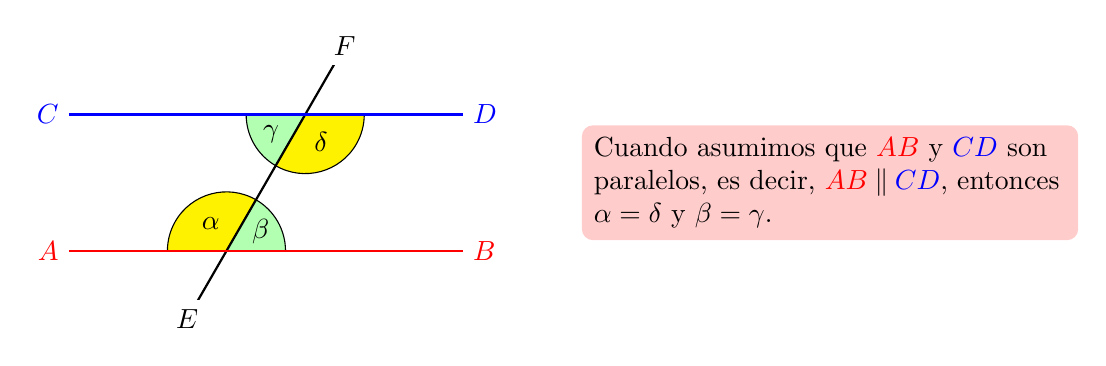
\begin{tikzpicture}
	  \draw[fill=yellow] (0,0) -- (60:.75cm) arc (60:180:.75cm);
	  \draw(120:0.4cm) node {$\alpha$};
	  \draw[fill=green!30] (0,0) -- (right:.75cm) arc (0:60:.75cm);
	  \draw(30:0.5cm) node {$\beta$};
	  \begin{scope}[shift={(60:2cm)}]
	    \draw[fill=green!30] (0,0) -- (180:.75cm) arc (180:240:.75cm);
	    \draw (30:-0.5cm) node {$\gamma$};
	    \draw[fill=yellow] (0,0) -- (240:.75cm) arc (240:360:.75cm);
	    \draw (-60:0.4cm) node {$\delta$};
	  \end{scope}
	  \begin{scope}[thick]
	    \draw  (60:-1cm) node[fill=white] {$E$} -- (60:3cm) node[fill=white] {$F$};
	    \draw[red]                   (-2,0) node[left] {$A$} -- (3,0) node[right]{$B$};
	    \draw[blue,shift={(60:2cm)}] (-3,0) node[left] {$C$} -- (2,0) node[right]{$D$};
	    \draw[shift={(60:1cm)},xshift=4cm]
	    node [right,text width=6cm,rounded corners,fill=red!20,inner sep=1ex]
	    {
	      Cuando asumimos que $\color{red}AB$ y $\color{blue}CD$ son paralelos, es decir, ${\color{red}AB} \mathbin{\|} \color{blue}CD$, entonces $\alpha = \delta$ y $\beta = \gamma$.
	    };
	  \end{scope}
	\end{tikzpicture}
\caption[Ejemplo de uso de PGF/Ti\textit{k}Z]{Ejemplo de uso de PGF/Ti\textit{k}Z, pero solo una muestra de sus capacidades.}
\label{F:tikz}
\end{figure}

Una buena cantidad de ejemplos están disponibles en \url{http://www.texample.net/tikz/} y la documentación (incluyendo un manual de uso de más de 700 páginas) está en \url{https://www.ctan.org/pkg/pgf?lang=en}.

%---------------------------------------
\subsection{Gráfico de datos y funciones con \texttt{pgfplots}}

%---------------------------------------
\subsection{Circuitos con Circuitikz}

El paquete \texttt{circuitikz} permite la creación de circuitos eléctricos y electrónicos. La Figura \ref{F:ampop} es un ejemplo.

\begin{figure}
  	\centering
		 \begin{circuitikz}[american]
		  \draw
		  % El amplificador operacional
		  (0,0) node[op amp] (opamp) {} node[] {{\tiny Amp Op}}
		  
		  % Las entradas
		  (opamp.-) node[circ] {} to[R, l_=$R_1$] ++(-2,0) node[ocirc] {} node[left] {$V_{s}$}
		  (opamp.+) -- ++(0,-0.5) node[ground] {} 
		  
		  % El lazo de realimentación
		  (opamp.-) -- ++(0,1)  to[R, l=$R_2$] ++(2,0) -| (opamp.out) {}
		  
		  % La salida
		  (opamp.out) -- ++(0.5,0) node[circ] {} to[R, l=$R_L$] ++(0,-2) to [short, i_=$I_o$] ++(0,0) node[ground] {}
		  (opamp.out) -- ++(1,0) node[ocirc] {} node[right]{$V_o$}
		  
		  ;
		\end{circuitikz}
    \caption[Amplificador inversor]{Amplificador inversor con un amplificador operacional cuya relación entrada--salida está dada por $V_o = -\frac{R_2}{R_1} V_s$.}
    \label{F:ampop}
\end{figure}

\begin{figure}
\centering
\begin{circuitikz}
\draw
	(0,0)
    	to [V, l=50~\si{\volt}] (0,2) to (0,3)
        to [R, l=$20~\si{\kilo\ohm}$] (5,3) to (5,2)
        to [vR, l=$R$] (5,0)
        to (0,0)
  	(0,2)
    	to [R, l_=$5~\si{\kilo\ohm}$] (5,2)     
;
\end{circuitikz}
\caption{Circuito básico.}
\label{F:circuitobasico}
\end{figure}

\begin{figure}
\centering
\begin{circuitikz}
\draw
	(0,0) node[ground]{}
    	to [V, l=(``Arenal'') $V_{1}$] (0,3)
        to [short] (0.5,3) node[circ]{}
   	(5.5,3)
        to [short] (5.5,4)
        to [R, l=$R_{1}$, i<=$I_{1}$] (3,4)
        to [cV, l=$v_{1}$] (0.5,4)
        to [short] (0.5,3)   
   	(6,3)
    	to [short] (5.5,3)
        to [short] (5.5,2)
        to [R, l=$R_{3}$, i<=$I_{2}$] (3,2)
        to [cV, l=$v_{3}$] (0.5,2)
        to [short] (0.5,3)
	(6,3) node[circ]{}
    	to [generic, i_=$I_{L}$, v^=$v_{L}$] (6,0) node[ground]{}
   	(6,3)
    	to [R, l=$R_{2}$, i<=$I_{3}$] (8.5,3)
        to [cV, l=$v_{2}$] (11,3)
    (11,0) node[ground]{}
        to [V, l_=$V_{2}$ (``Miravalles'')] (11,3)
;
\end{circuitikz}
\caption[Circuito de transmisión de potencia]{Circuito de transmisión de potencia por varias líneas conductoras desde centros de generación y con sistemas de ajuste de la corriente.}
\label{F:transmisionpotencia}
\end{figure}

\begin{figure}
\centering
\begin{circuitikz}
\draw 
(0,0)	to [battery, l_=$V_i$] (0,3)
		to [R, l_=$R_1$] (2.5,3)
        to [cV, l_=$A v_x$] (5,3)
        to [short] (6,3)
        to [vR, l_=$R_T$, i=$i_{R_T}$] (6,0) node[ground]{}
        to [short] (0,0)
(6,3)	to [short] (7,3)
(6,0)	to [short] (7,0)

;
\draw (2.5,3) to [open, v=$v_x$] (2.5,0);
\draw (2.5,3) node[circ]{};
\draw (2.5,0) node[circ]{};

\draw[dashed] (-0.8,-0.8) rectangle (4.8,3.8);
\draw (-0.8,-0.8) node [above right]{Fuente de corriente};

\draw (7,-0.5) rectangle (9,3.5);
\draw (8,1.5) node [align=center]{Circuito \\ de acople};

\draw 
(9,3)	to [short] (10,3)
		to [R, l_=$R_2$] (12,3)
		to [generic, l_=$Y$, v^=$v_Y$] (14,3)
(9,0)   to [short] (14,0) node[ground]{}
		to [cV, l=$A v_z$] (14,3)
(14,0)	to [short] (15.3,0)
		to [open, v>=$v_o$] (15.3,3)
		to [short] (14,3)
;
\draw (12,3)	to [open, v=$v_z$] (12,0);
\draw (12,3) node[circ]{};
\draw (12,0) node[circ]{};

\draw[dashed] (9.8,-0.8) rectangle (14.8,3.8);
\draw (9.8,-0.8) node [above right]{Amplificador};

\draw (15.3,3) node[circ]{} node[right]{$a$};
\draw (15.3,0) node[circ]{} node[right]{$b$};
\end{circuitikz}
\caption[Circuito de acondicionamiento y amplificación]{Circuito de acondicionamiento y amplificación de la señal de un sensor resistivo $R_T$, dependiente de la temperatura.}
\label{F:acondicionamiento}
\end{figure}

\begin{figure}
\centering
\begin{circuitikz}

% PNP Q1
\draw
	(0,4) 	node[pnp,rotate=90](Q1){} node[above]{$Q_1$}
;
% NPN Q2
\draw
	(0,1.5) 	node[npn,rotate=180,yscale=-1](Q2){} node[left]{$Q_2$}
;
% Op Amp
\draw
	(3,1.5) 	node[op amp,rotate=180,yscale=-1](CMP){} node[]{AMP}
;
% Resistores
\draw
	(6,4) node[circ]{} 
    	to [R, l=$R_1$] (6,2) 
    	to [R, l=$R_2$] (6,0) node[ground]{}
;
% Conectores
\draw
	(-1.5,4) 	node[ocirc]{} node[above]{$V_{IN}$} 
    		to [short] (Q1.emitter)
  	(Q1.base) to [short] (Q2.collector)
    (Q2.emitter) to [short] (0,0) node[ground]{}
    (CMP.out) to [short] (Q2.base)
    (Q1.collector) to [short] (7,4) node[ocirc]{} node[above]{$V_{OUT}$}
    (CMP.-) to [short] (6,2) node[circ]{}
    (4.5,0) node[ground]{} to [battery,l_=$V_{R}$] (4.5,1) to [short] (CMP.+) 
;
\end{circuitikz}
\caption{Regulador lineal de tensión con lazo de control.}
\label{F:reguladorlineal}
\end{figure}

\begin{figure}
\centering
\begin{circuitikz} 
\draw
	(0,0) node[op amp,yscale=-1] (opamp) {}
    (0,0) node[](){CMP}
;

\draw 
	(-4.5,2) node[rground, yscale=-1](){} 
    to [I, l_=$I$] (-4.5,1)
    to [short,-*] (-4.5,0.5)
    to [short] (-4.5,-1.8) 
;

\draw 
	(-3,2) node[rground, yscale=-1](){} 
    to [I, l_=$I$] (-3,1)
    to [short,-*] (-3,-0.5) 
    to [R, l_=$R_1$] (-3,-2.5)
    to [R, l_=$R_2$] (-3,-4.5) node[ground](){}
;

\draw 
	(-3,-2.5) to [short,*-] (-2,-2.5)
    to [cspst,] (-2,-4.5) 
    to [short] (-3,-4.5)
    (-1.8,-3.8) node[right](){SW}
;

\draw 
	(-4.5,-2.5) node[pnp](pnp){}
	(pnp.base) node[anchor=east] {\tiny{B}}
    to [short] (-5.3,-4.5) to [short,-*] (-4.5,-4.5)
    (pnp.emitter) node[anchor=east]{\tiny{E}} 
    (pnp.collector) node[anchor=east] {\tiny{C}}
    to [short] (-4.5,-4.5) to [short,-*] (-3,-4.5)
    (-4.5,-2.5) node[anchor=west] {$Q_T$}
;

\draw (opamp.-) to [short] (-3,-0.5) node[anchor=east]{$V^-$};
\draw (opamp.+) to [short] (-4.5,0.5) node[anchor=east]{$V^+$};
\draw (opamp.out) to [short] (1.5,0);
\draw[dashed] (1.5,0) -- (1.5,-3.4) -- (-1.7,-3.4);

\draw (4,0)  node[ocirc]{} node[anchor=south]{\={S}} to [full diode] (1.5,0) node[circ]{} node[anchor=south]{$V_{\mathrm{CMP}}$};

\end{circuitikz}
\caption{Circuito para protección térmica con lazo de histéresis.}
\label{F:protecciontermica}
\end{figure}

\subsection{Inserción de código fuente}
%%%%%%%%%%%%%%%%%%%%%%%%%%%%%%%%%%%%%%%

En ocasiones es necesario introducir secciones de código fuente de programación dentro de reportes. La inserción es especial, pues el compilador no debe confundir las instrucciones dentro del código con instrucciones de \LaTeX. Además, se prefiere un formato específico con resaltado de sintaxis para mejorar la legibilidad (como en los editores de código o en los IDE). Un paquete que provee soluciones para este requisito es \texttt{listings}.

Para el código fuente hecho en Matlab es posible utilizar el paquete \texttt{mcode} (adjunto como archivo a la carpeta que contiene el proyecto) que asigna a \texttt{listings} el formato apropiado, como se ve en el siguiente código:

\lstinputlisting[inputencoding=latin1]{codigo/codigoejemplo.m}

%%%%%%%%%%%%%%%%%%%%%%%%%%%%%%%%%
\section{Referencias para \LaTeX}
%%%%%%%%%%%%%%%%%%%%%%%%%%%%%%%%%

La comunidad de usuarios de \LaTeX~ es grande y colaborativa. Hay multitud de recursos en línea para aprender buenas prácticas y ``trucos'' para mejorar los documentos. Algunas de las mejores referencias son:

\begin{description}
\item[Wikibook] \url{https://en.wikibooks.org/wiki/LaTeX}
\item[Cookbook] \url{http://latex-cookbook.net/}
\item[TeXample] \url{http://texample.net/}
\item[HowtoTeX] \url{http://www.howtotex.com/}
\item[Font Catalogue] \url{http://www.tug.dk/FontCatalogue/}
\end{description}

\subsection{¿Dónde editar \LaTeX?}\label{S:programas}
%%%%%%%%%%%%%%%%%%%%%%%%%%%%%%%%%%%%%%%%%%%

\paragraph{Editores de texto ``de escritorio''}

Existen varios programas para la edición y compilación de archivos de \LaTeX. Se ha escogido Texmaker debido a que es multiplataforma (Mac, Linux, Windows) y cuenta con otras características como resaltado de sintaxis, autocompletar, corrección ortográfica, asistente para la creación de documentos, accesos rápidos a símbolos, comandos y entornos, entre otros. Se puede, claro está, editar el documento con cualquier editor y compilar, siempre y cuando se tengan los paquetes necesarios\footnote{Esta es una ventaja de ser un código estándar abierto.}.

En Windows, junto con Texmaker debe instalarse MiKTeX, que es un conjunto de paquetes, fuentes y demás necesarios para compilar el archivo.

Ambos están disponibles para descarga gratuita desde \url{http://miktex.org/} y \url{http://www.xm1math.net/texmaker/}.

Una base de datos extensiva de los paquetes de \LaTeX~ está en \url{http://www.ctan.org/}. Es especialmente útil para encontrar la documentación de los paquetes. Desde esta página se pueden descargar los paquetes, pero la mejor forma de revisar los paquetes disponibles e instalarlos fácilmente es a través del \emph{MiKTeX Package Manager}, disponible después de instalar el MiKTeX.

\paragraph{Plataformas en línea de edición para \LaTeX}

Una alternativa muy popular de años muy recientes es la edición en línea. Entre las ventajas se encuentran: almacenamiento en línea, edición colaborativa, herramientas web (bibliografías y otros), compilación simultánea, más la mayoría de las otras ventajas de los editores ``de escritorio'' como autocompletar, símbolos, etc.

Los editores más populares son:

\begin{description}
\item[Overleaf] \url{https://www.overleaf.com/}
\item[ShareLaTeX] \url{https://www.sharelatex.com/}
\item[Papeeria] \url{https://papeeria.com/}
\end{description}
% ----------------------------------------
  \chapter{Conclusiones y recomendaciones}
% ----------------------------------------
\label{C:conclusiones}

El informe debe terminarse con la enumeración de las principales conclusiones derivados del trabajo realizado.  En particular, debe verificarse el cumplimiento de los objetivos planteados para el mismo.

\section{Conclusiones}
El aporte (\emph{novedad}) hecho con el proyecto, debe destacarse.

Las conclusiones pueden enumerarse en forma suscinta como una lista, ya sea itemizada o numerada.

\section{Recomendaciones}
Con base en las trabajo realizado y las conclusiones sobre el mismo, puede ser necesario incluir una sección, o lista, de recomendaciones.  Por ejemplo, sobre la utilización de otro enfoque para resolver el problema.

% 8. APÉNDICES
\appendix
\chapter{Apéndice de ejemplo}

\lipsum[3]

\section{Una sección del apéndice}

\lipsum[4]

\subsection{Y una sub-sección}

\lipsum[5-8]

\subsection{Y otra sub-sección}

\lipsum[5-8]
\chapter{Un apéndice ejemplo con archivo anexo}

Para insertar archivos \texttt{.pdf} se utiliza el paquete \texttt{pdfpages}. Este paquete tiene opciones disponibles para la configuración del documento inserto.

Aquí hay dos ejemplos sencillos.

%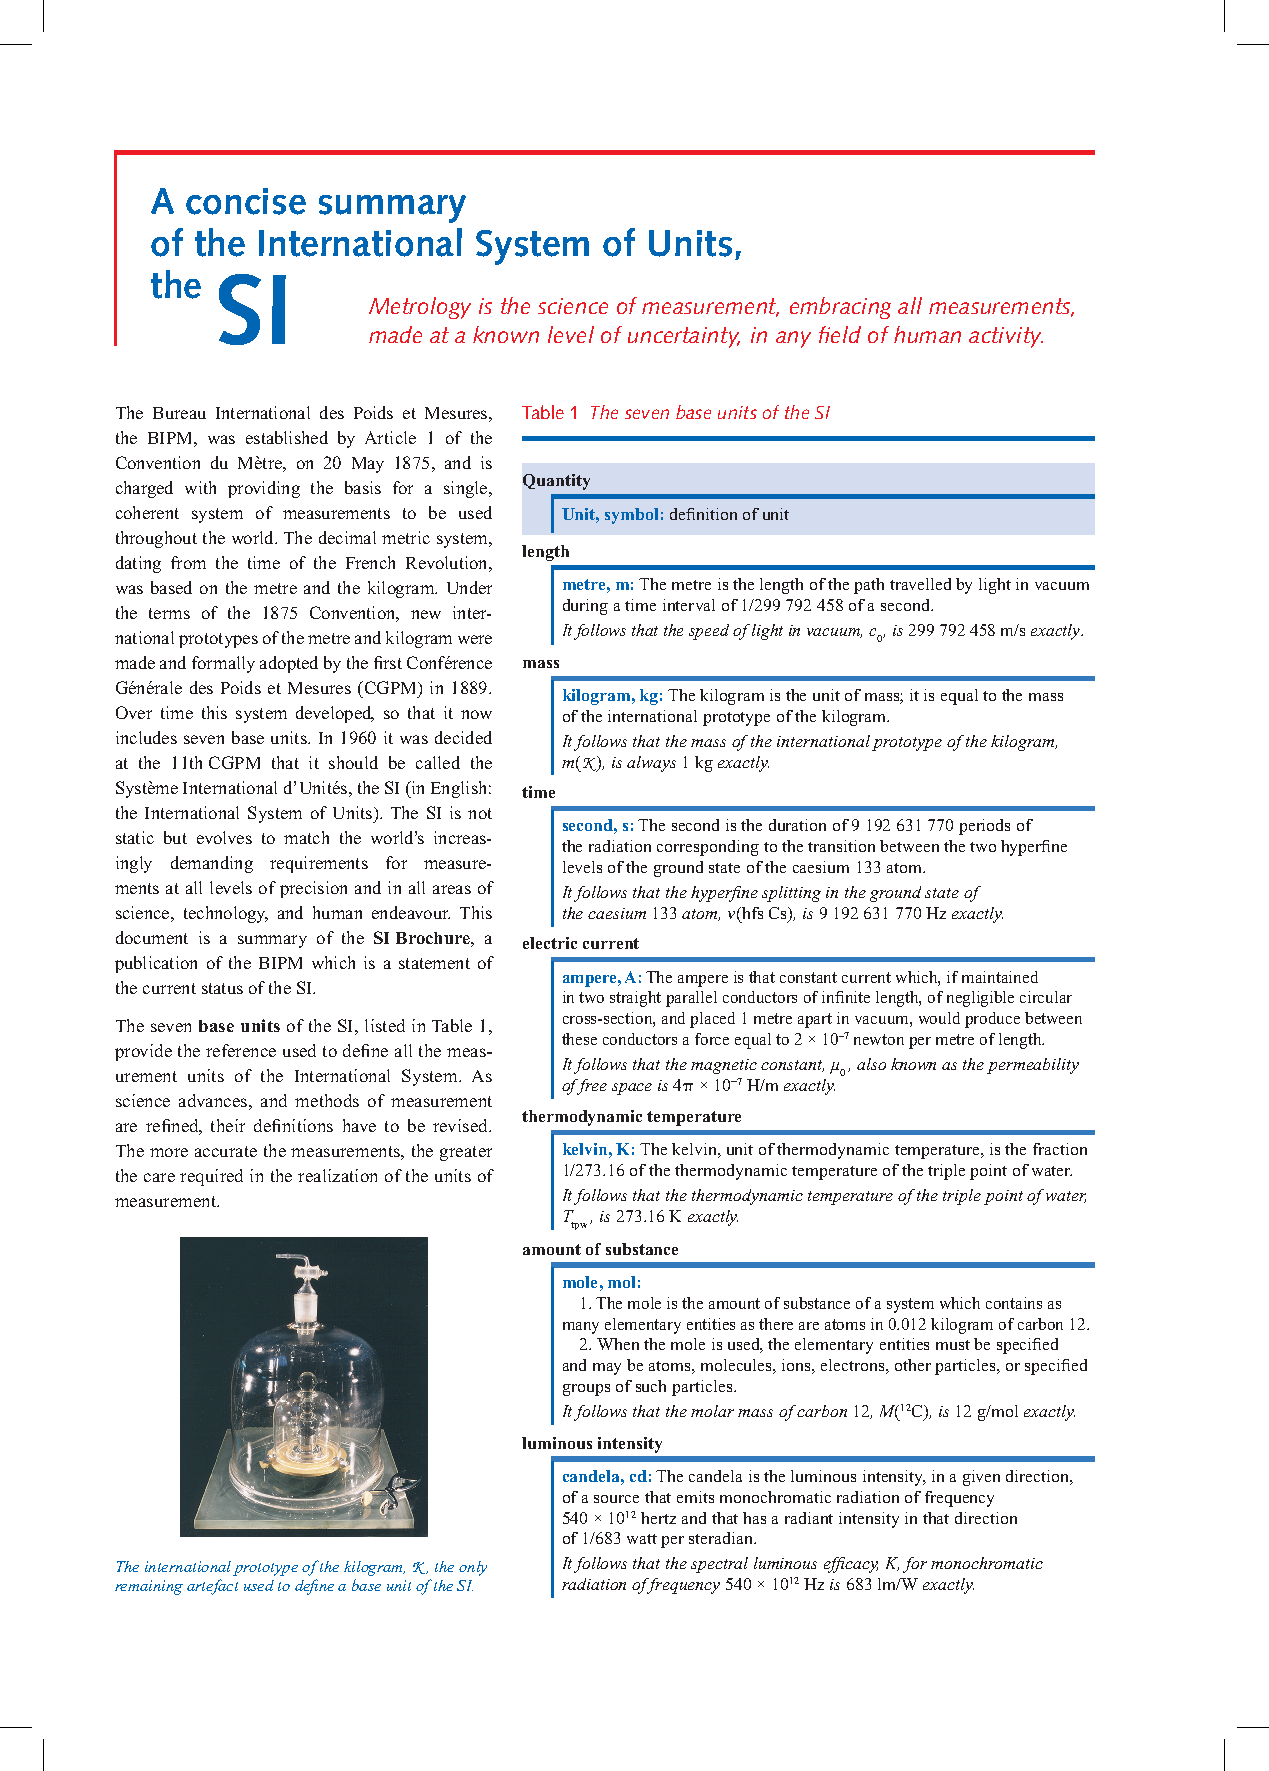
\includepdf[pages=-,nup=2x2]{apendices/SIsummary.pdf}

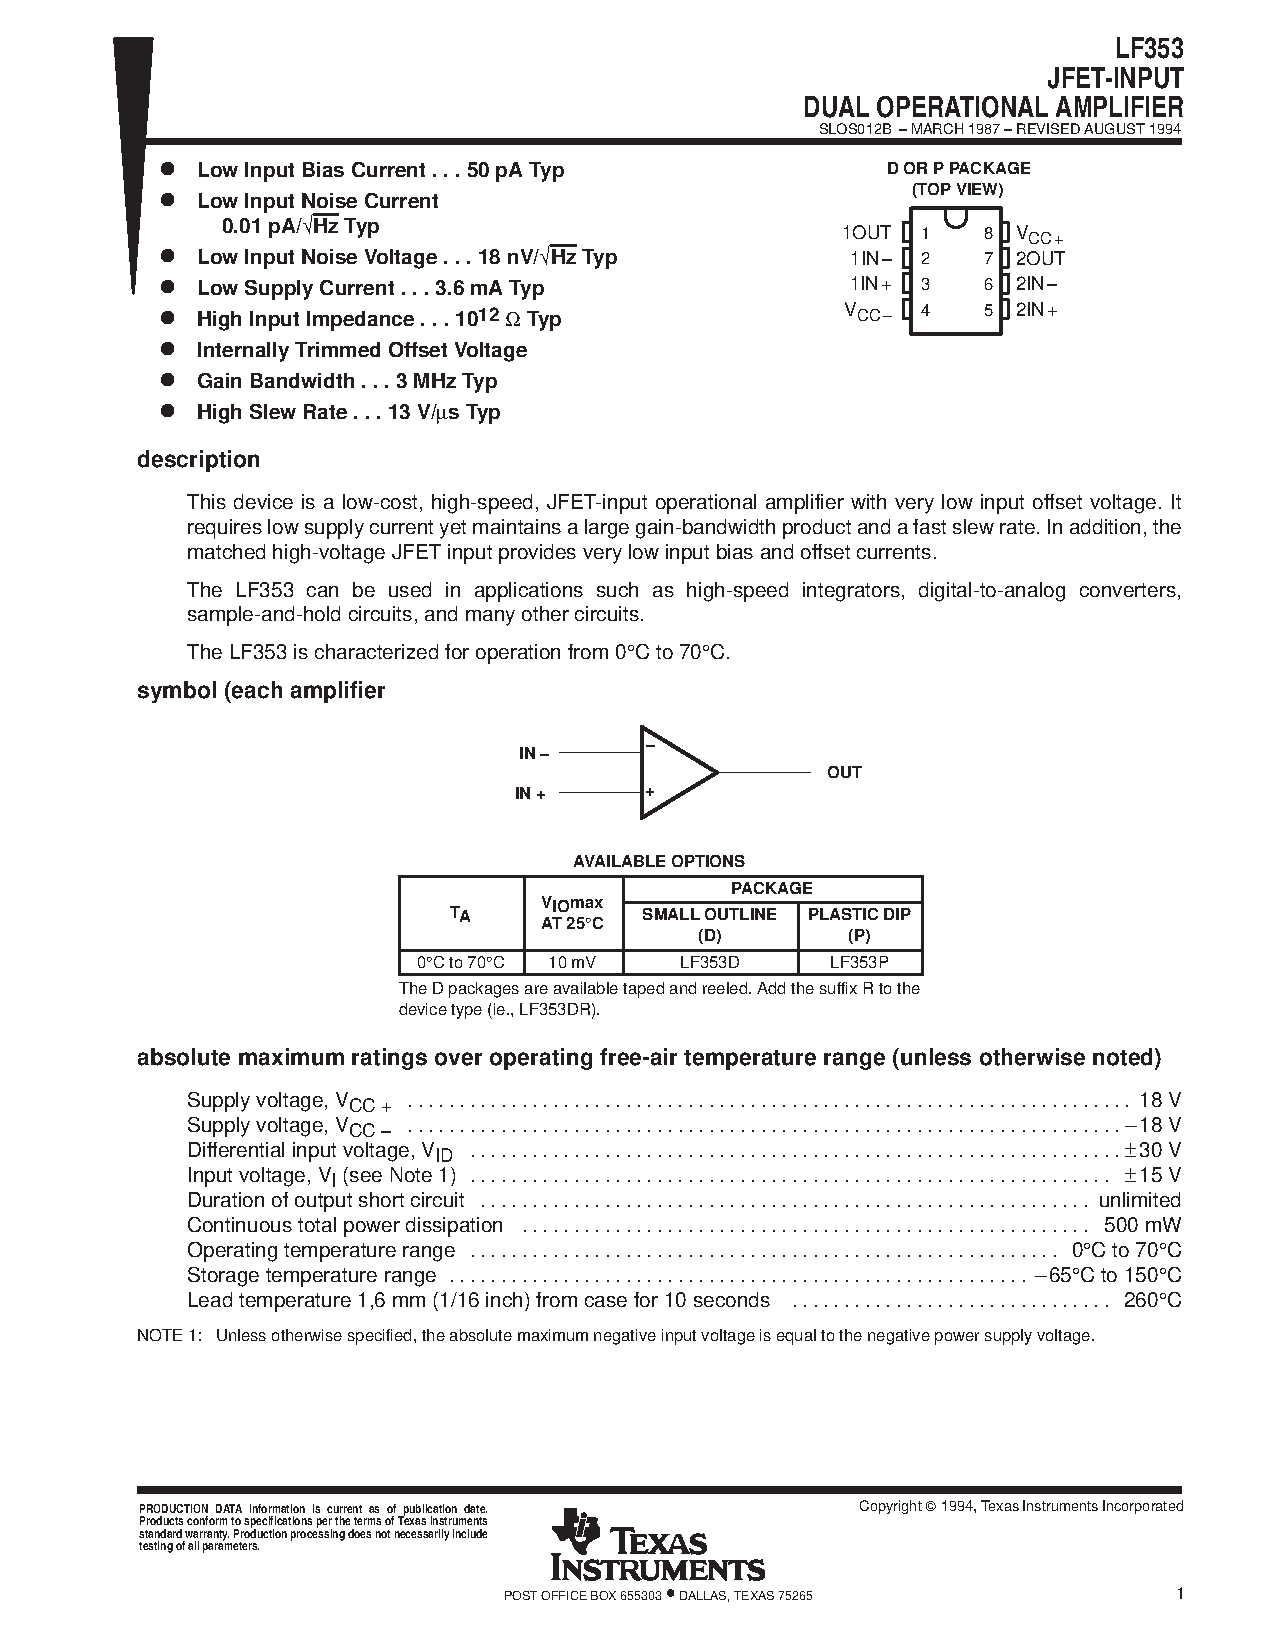
\includepdf[pages=1]{apendices/LF353.pdf}

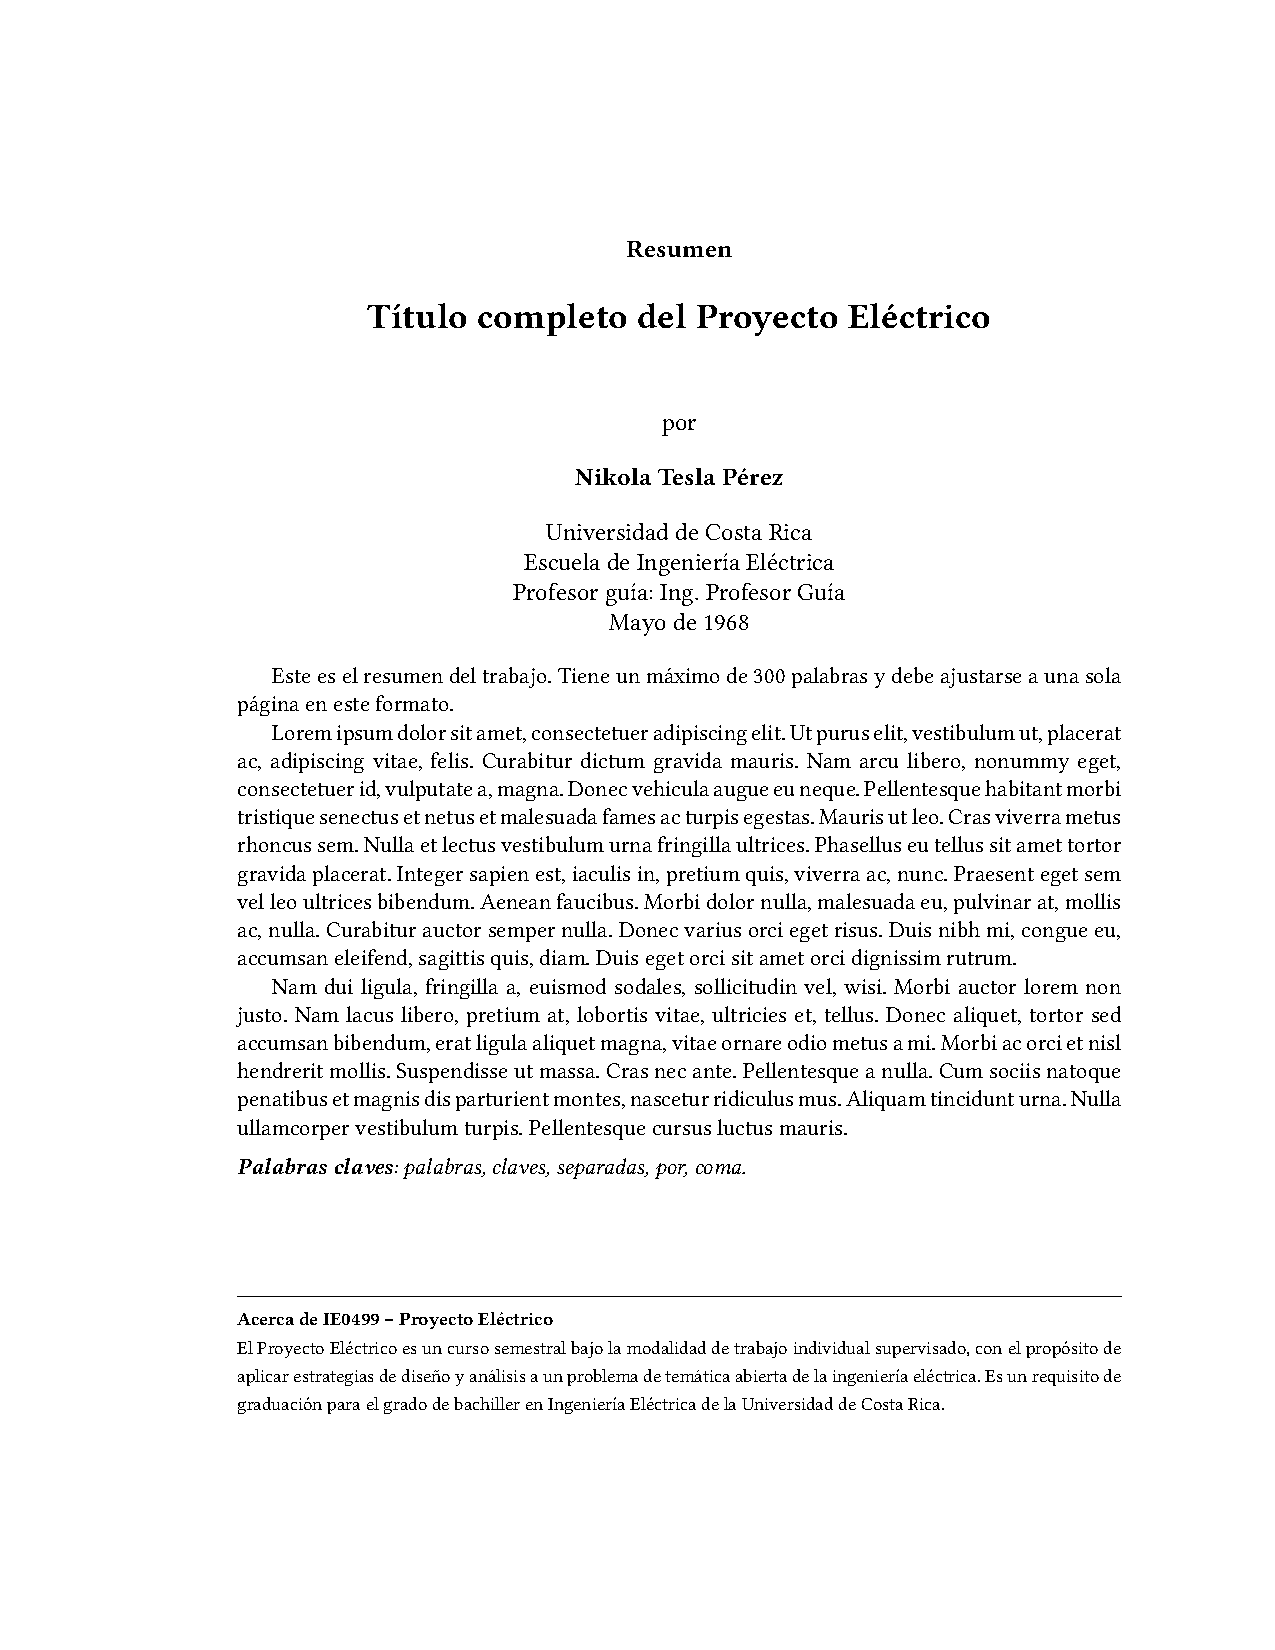
\includepdf[pages=-,scale=0.6,pagecommand={}]{apendices/Resumen.pdf}

\backmatter

% 9. BILIOGRAFÍA
\bibliographystyle{plain}
\bibliography{bibliografia/bibliografia.bib}

%%%%%%%%%%%%%%%%%%%
\end{document}
%%%%%%%%%%%%%%%%%%%
\end{verbatim}

%%%%%%%%%%%%%%%%%%%%%%%%%%%%%%%%%%%%%%%%%%%%%%
\section{Las partes de un documento de \LaTeX}
%%%%%%%%%%%%%%%%%%%%%%%%%%%%%%%%%%%%%%%%%%%%%%

\subsection{Preámbulo y cuerpo del documento}
%%%%%%%%%%%%%%%%%%%%%%%%%%%%%%%%%%%%%%%%%%%%%

Los archivos \texttt{.tex} de donde se generan los documentos en \LaTeX~ tienen dos grandes secciones: el encabezado o preámbulo y el cuerpo del documento.

En el \textbf{encabezado} del documento se definen los parámetros más importantes del documento, y se invocan los ``paquetes'' que permiten la edición de características especiales. Entre las características que se pueden definir aquí están: tamaño del papel, tamaño y tipo de tipografía, tipo de documento (reporte, artículo, libro, carta\ldots), numeración, autor, fecha, título y más. 

Además de estas definiciones generales, se deben cargar todos los \textbf{paquetes} que permiten hacer ediciones especiales como: introducir hipervínculos, agregar colores, agregar imágenes, editar encabezados y pies de página, etc. 

Para utilizar un paquete se escribe la instrucción \verb+\usepackage[opciones]{nombredelpaquete}+, donde las opciones están definidas por cada paquete particular. 

Por ejemplo \verb+\usepackage[spanish]{babel}+. El paquete Babel permite cambiar la lengua del documento (en inglés por defecto), y entre paréntesis cuadrado se especifica que sea español.

Los paquetes que utiliza \LaTeX~ están en un repositorio (ver Sección \ref{S:programas}). La documentación de los paquetes puede encontrarse en la página de CTAN (\textit{Comprehensive TEX Archive Network}), \url{https://www.ctan.org/}.

Uno de los elementos más importantes de \LaTeX~ es el \emph{entorno}. Un entorno (\emph{environment}) siempre inicia con \verb+\begin{nombredelentorno}+ y finaliza con \verb+\end{nombredelentorno}+. Dentro de él, todo el contenido va a tener un formato característico dependiendo del tipo de entorno. Las ecuaciones, figuras y tablas tienen su propio entorno. Hay otros para listas numeradas, resumen, teoremas, texto centrado\ y más. El mismo cuerpo del documento es un gran entorno \texttt{document}.

A continuación se describirá el uso de algunos de los entornos más importantes: ecuaciones, tablas y figuras.

\subsection{Ecuaciones}
%%%%%%%%%%%%%%%%%%%%%%%

Hay tres tipos de ecuaciones posibles: unas en línea, o dentro del párrafo, otras en modo \emph{display} con numeración y sin numeración. 

\begin{description}

\item [Las ecuaciones en línea] están rodeadas por los símbolos \verb+$ $+ (una forma abreviada de crear el entorno). Se utilizan cuando se coloca una fórmula en un párrafo, por ejemplo $ {{B}_{f}}\ge 0,2 $, que no lleva numeración y que debe estar alineada con el texto. \LaTeX~ se encargará de ajustar su tamaño y ubicación, como cuando se introduce una raíz cuadrada $ \sqrt {{b^2} - 4ac} $ o una integral  $ \int_0^\infty e^{-x}\,\mathrm{d}x $. 

\item [Las ecuaciones numeradas] se hacen dentro del entorno \texttt{equation}. Ejemplos de ecuaciones se muestran a continuación.

\begin{verbatim}
\begin{equation}
x_{1,2} = \frac{-b \pm \sqrt{b^2 - 4ac}}{2a}
\end{equation}
\end{verbatim}

\begin{equation}
x_{1,2} = \frac{-b \pm \sqrt{b^2 - 4ac}}{2a}
\end{equation}

\begin{equation}\label{E:desigualdad}
{B}_{f}\ge 0,2
\end{equation}

\begin{equation}\label{E:anchodebanda}
BW\ge 500\text{ MHz}
\end{equation}

donde $ {B}_{f} $ es el ancho de banda fraccional y se define como:

\begin{equation}\label{E:fraccional}
{{B}_{f}}=\frac{BW}{{{f}_{c}}}=\frac{\left( {{f}_{H}}-{{f}_{L}} \right)}{{\left( {{f}_{H}}+{{f}_{L}} \right)}/{2}\;}
\end{equation}

donde $f_H$ y $f_L$ son las frecuencias superior e inferior de la banda de transmisión de -10 dB, $ BW $ es el ancho de banda y $f_c$ la frecuencia central.

El estilo de la numeración depende del tipo de documento (\texttt{article}, \texttt{report}, \texttt{book}\ldots) y obedecerá (si no se especifica lo contrario) la secuencia numérica.

\item [La ecuaciones no numeradas] se deben utilizar en ocasiones, sobre todo cuando se trata de pasos intermedios o cálculos y no la deducción de alguna expresión. Para ello se deben utilizar los símbolos \verb+\[+ y \verb+\]+ (otra forma abreviada de crear el entorno) para rodear la ecuación.

\[
 \lim_{x \to \infty} \exp(-x) = 0
\]

\[
 R_{pu} = 2,7~\si{\kilo\ohm}
\]

\end{description}

Será necesario también en ocasiones incluir texto dentro de las ecuaciones. Pero es necesario escribir este texto dentro de los comandos \verb+\text{}+, \verb+\textbf{}+ o similares, para que se les aplique el espaciado y formato correctos. De otro modo sucede lo que se muestra en la ecuación (\ref{E:sintexto}), mientras que la ecuación (\ref{E:contexto}) muestra el uso corregido, incluyendo cierto formato añadido para resaltar.

\begin{equation}\label{E:sintexto}
Ciclo de trabajo = \frac{Tiempo en alto}{Per\acute{i}odo}
\end{equation}

\begin{equation}\label{E:contexto}
\text{Ciclo de trabajo} = \frac{\textsf{Tiempo en alto}}{\textbf{Per\'{i}odo}}
\end{equation}

A pesar de que la escritura de ecuaciones directamente en \LaTeX~ puede resultar algo complicada al principio, basta con una rápida investigación en la vasta información de las referencias suministradas y en la red\footnote{Hay muchas comunidades de usuarios en internet en foros y demás que resuelven estos problemas típicos} para encontrar la forma de realizar la ecuación deseada. Como alternativa, se puede utilizar un editor gráfico de ecuaciones como \href{http://www.dessci.com/en/products/mathtype/}{MathType} y de ahí exportar a \LaTeX\footnote{Para hacerlo: en la ventana de edición de ecuaciones de MathType se debe ir a \textsf{Preferences / Cut and Copy Preferences}, en la ventana emergente se debe seleccionar la opción \textsf{MathML or TeX} y en la lista desplegable escoger \textsf{LaTeX 2.09 and later}. En la misma ventana de edición se selecciona y copia la ecuación. La barra de estado mostrará: \textsf{Translated (LaTeX 2.09 and later)}.}. Es necesario, aún así, aprender los comandos básicos que facilitan y hacen más rápida la composición de fórmulas.

También se pueden editar ecuaciones en la aplicación en internet disponible en \url{http://rinconmatematico.com/latexrender/} en la cual se puede ver el resultado de la ecuación editada.

\subsection{Figuras}\label{S:Figuras}
%%%%%%%%%%%%%%%%%%%%%%%%%%%%%%%%%%%%%

Para las figuras existe un entorno llamado \verb+figure+, dentro del cual se ubican y configuran las imágenes.

Para ``llamar'' al archivo se debe hacer una referencia a su ubicación. Si está ubicada en la misma carpeta del documento se escribe \verb+nombre_de_la_imagen.jpg+\footnote{O cualquier formato de imágenes soportado, como .png, .gif y otros}. Pero los archivos de imágenes, de preferencia y por una cuestión de orden, deben colocarse dentro de una carpeta dedicada. Entonces, si está dentro de una carpeta se indica \verb+./carpeta/nombre_de_la_imagen.jpg+. Para subir un nivel en las carpetas se utiliza \verb+../carpeta/subcarpeta/nombre_de_la_imagen.jpg+. 

La imagen ``Nube de tormenta con rayos y lluvia'' es un ejemplo de imagen insertada.

\begin{figure}[H]
\centering
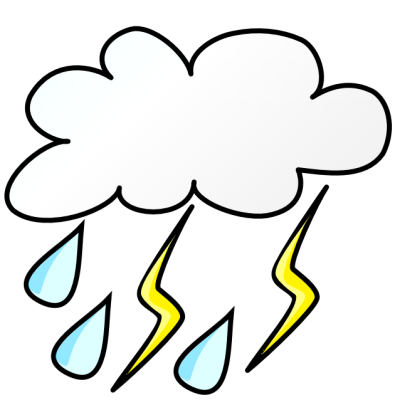
\includegraphics[width=0.2\textwidth]{./imagenes/tormenta.png} 
\caption{Nube de tormenta con rayos y lluvia}
\label{F:tormenta}
\end{figure}

La instrucción para insertar la gráfica es:


\begin{lstlisting}[]
\begin{figure}[H]
\centering
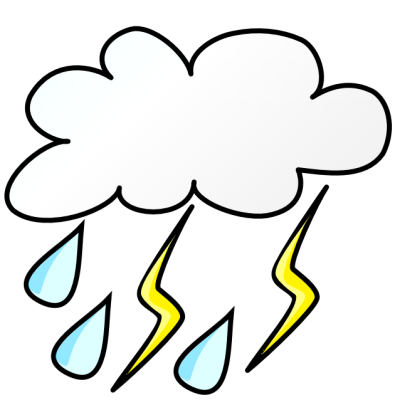
\includegraphics[width=0.2\textwidth]{./imagenes/tormenta.png} 
\caption{Nube de tormenta con rayos y lluvia}
\label{F:tormenta}
\end{figure}
\end{lstlisting}

La descripción es la siguiente:

\begin{itemize}\itemsep0pt \parskip0pt \parsep0pt
\item \verb+\begin{figure}[H]+ en la línea 1 inicia el entorno de la figura y declara que será ubicada inmediatamente luego del texto, con \verb+[H]+.
\item \verb+\centering+ en la línea 2 es una instrucción abreviada para indicar que la figura estará centrada.
\item \verb+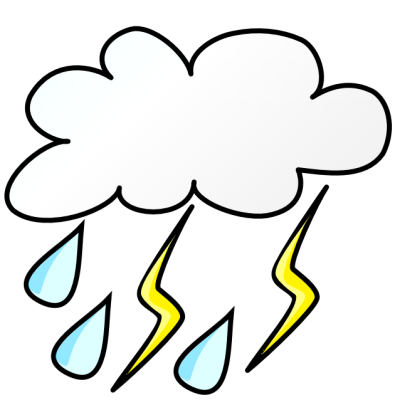
\includegraphics[width=0.2\textwidth]{./imagenes/tormenta.png}+ es la instrucción para insertar el archivo de la imagen, junto con indicaciones adicionales sobre el tamaño (un 20 \% del ancho del texto).
\item \verb+\caption{Nube de tormenta con rayos y lluvia}+ la instrucción  \texttt{caption}\footnote{En inglés, es bastante explícita esta instrucción, y en general puede decirse lo mismo de todos los comandos de \LaTeX, (ver por ejemplo \textsf{footnote}, \textsf{includegraphics}, \textsf{subsection}, etc.)} es el pie de figura con el nombre y la explicación. El número de figura lo inserta \LaTeX~ automáticamente.
\item \verb+\label{F:tormenta}+ es una etiqueta para referencia dentro de otras partes del texto.
\item \verb+\end{figure}+ cierra el entorno de la figura.
\end{itemize}

Como buena práctica, se recomienda nombrar el archivo de la imagen igual que la etiqueta, y con \textit{un nombre representativo}. Los nombres no deben tener espacios ni tildes ni eñes. Por ejemplo: \verb+senal_entrada_sinusoidal.jpg+.

\LaTeX, por defecto, va a ubicar las imágenes arriba o debajo de la página, y no inmediatamente después del texto en el que se escribe dentro del código, excepto que se indique lo contrario con \verb+\begin{figure}[h!]+ o con \verb+\begin{table}[H]+ utilizando el paquete \verb+float+.

Adicionalmente, se puede ubicar varias imágenes dentro de un mismo entorno de figura, como en la Figura \ref{F:subfiguras}. Ahí se muestran cuatro figuras distintas dentro del mismo entorno, donde se puede hacer referencia al transistor en \ref{F:subfig1}, al LED en \ref{F:subfig2}, al fotoconductor en \ref{F:subfig3} y al circuito integrado en \ref{F:subfig4}.

\begin{figure}[h!]
\centering
\subfloat[Transistor (texto que aparece en el índice)][Transistor en encapsulado TO-220]{
	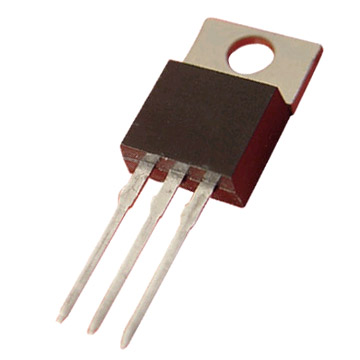
\includegraphics[width=0.2\textwidth]{./imagenes/transistor.jpg}
	\label{F:subfig1}}
\qquad
\subfloat[LED][LED blanco de baja potencia]{
	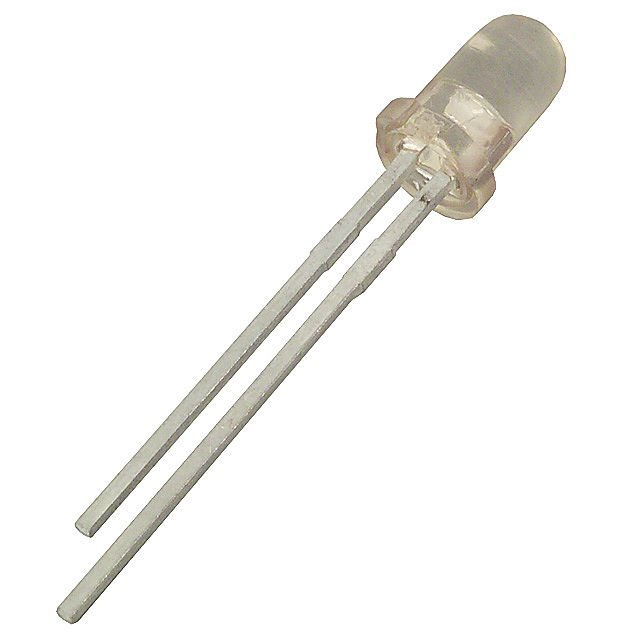
\includegraphics[width=0.2\textwidth]{./imagenes/led.jpg}
	\label{F:subfig2}}
\\
\subfloat[Fotoconductor][Fotoconductor]{
	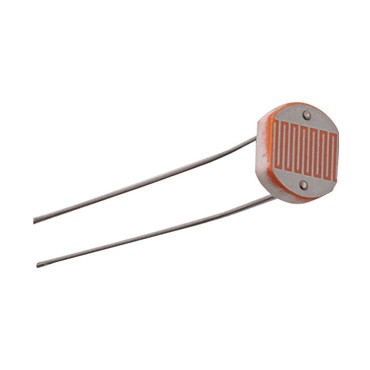
\includegraphics[width=0.2\textwidth]{./imagenes/fotoconductor.jpg}
	\label{F:subfig3}}
\qquad
\subfloat[Circuito integrado][Circuito integrado en encapsulado DIP-8]{
	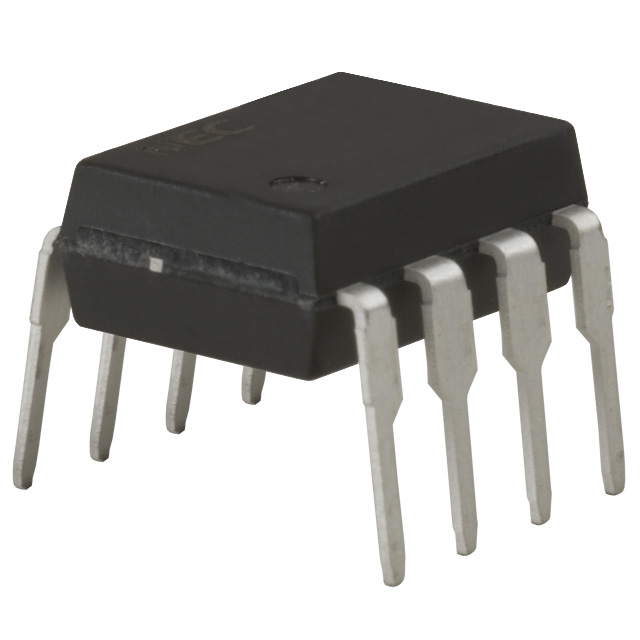
\includegraphics[width=0.2\textwidth]{./imagenes/integrado.jpg}
	\label{F:subfig4}}
\caption{Una figura con varias subfiguras, utilizando el paquete \texttt{subfig}}
\label{F:subfiguras}
\end{figure}

\subsection{Tablas}
%%%%%%%%%%%%%%%%%%%

Para las tablas se debe utilizar el entorno \verb+table+.

Aquí hay dos casos posibles:

\begin{description}

\item [Que la tabla debe construirse en \LaTeX] y en ese caso se debe usar el entorno \verb+tabular+, que a su vez se incluye dentro de \verb+table+.

\item [Que la tabla es en realidad una imagen] si fue generada por otro programa o fue escaneada, etc. Esta imagen entonces se incluye dentro del entorno \verb+table+ para que sea tratada como tal (y se numere como tabla, y se incluya en el índice de tablas, y se hagan las referencias como tablas, etc.).

\end{description}

Como ejemplo sencillo, la Tabla \ref{T:ejemplo} muestra una tabla con líneas verticales, declaradas como \verb+c | c+, que significa \textit{centrado - línea vertical - centrado}, y líneas horizontales, declaradas como \verb+\hline+ después de cada línea salto de línea (\verb+\\+).

\begin{table}
\caption{Comparación de velocidad de UWB con otros estándares alámbricos e inalámbricos}
\label{T:ejemplo}
\begin{center}
\begin{tabular}{ c | c}
\hline
\textbf{Velocidad [Mbits/s]} & \textbf{Estándar} \\ 
\hline
480 & UWB, USB 2.0 \\ 
200 & UWB (4 m) \\
110 & UWB (10 m) \\ 
90 & Fast Ethernet \\ 
54 & 802.11a \\ 
20 & 802.11g \\ 
11 & 802.11b \\ 
10 & Ethernet \\ 
3 & Bluetooth \\ 
0,256 & ZigBee \\ 
\hline
\end{tabular}
\end{center}
\end{table}

La instrucción \verb+\begin{tabular}{ | c | c |}+ genera un cuadro con líneas verticales en ambos lados, como en la Tabla \ref{T:ejemploconlineas}. 

Cuando se tiene un documento de dos o más columnas, es importante notar que una tabla puede ser muy grande y no quepa en una sola columna, por tanto debe especificarse que se acomode a todo lo ancho de la página. Esto es sencillo: basta con escribir \verb+table*+ al inicio y al final cuando se declara el entorno en \verb+\begin{} ... \end{}+.

\begin{table*}
\caption[Título en el índice]{Título que aparece en el pie de figura o encabezado de la tabla. Puede ser bastante amplio y explicar con más detalle. Debido a que el título que aparece en el índice es corto, no hay problema de que se exceda el espacio apropiado ahí.}
\label{T:ejemploconlineas}
\begin{center}
\begin{tabular}{| c | c |}
\hline
\textbf{Velocidad [Mbits/s]} & \textbf{Estándar} \\ 
\hline
480 & UWB, USB 2.0 \\ 
200 & UWB (4 m), 1394a (4,5 m) \\
110 & UWB (10 m) \\ 
90 & Fast Ethernet \\ 
54 & 802.11a \\ 
20 & 802.11g \\ 
11 & 802.11b \\ 
10 & Ethernet \\ 
3 & Bluetooth \\ 
0,256 & ZigBee \\ 
\hline
\end{tabular}
\end{center}
\end{table*}

Del mismo modo que en las figuras, \LaTeX~ por defecto colocará la tabla en la parte superior de la siguiente página, excepto que se indique lo contrario (con \verb+\begin{table}[h!]+)\footnote{Para mejor manejo de la posición de figuras, tablas y otros, utilizar el paquete \textsf{float}}.

\begin{table}
\caption{Otra tabla utilizando el paquete \texttt{booktabs}}
\label{T:otratabla}
\centering
\begin{tabular}{c l r r}
\toprule
\multicolumn{2}{c}{Producto} \\
\cmidrule(r){1-2}
Cantidad & Descripción & Precio unitario & Precio total  \\
\midrule
3  & Transistores 	& 250	& 750	\\
4  & Osciladores   	& 500   & 2000 \\
3  & Amp Ops     	& 600   & 1800	\\
10 & Resistores  	& 25    & 250	\\
10 & Capacitores	& 50 	& 500	\\
\midrule 
\multicolumn{3}{r}{TOTAL} & \textbf{5300} \\
\bottomrule
\end{tabular}
\end{table}

%%%%%%%%%%%%%%%%%%%%%%%%%%%%%
\section{Herramientas útiles}
%%%%%%%%%%%%%%%%%%%%%%%%%%%%%

%----------------------------------
\subsection{Referencias a figuras, tablas, ecuaciones, secciones y otros}

Es fundamental a lo largo del texto hacer referencias a figuras, tablas, ecuaciones, secciones y otros. Todos estos elementos tienen una etiqueta \verb+\label{}+ asociada a cada uno. 

La instrucción para hacer la referencia a esta etiqueta es \verb+\ref{}+.

Así entonces, se puede hacer referencia a las ecuaciones (\ref{E:desigualdad}), (\ref{E:anchodebanda}) y (\ref{E:fraccional}), a la Figura \ref{F:tormenta} y a la Tabla \ref{T:ejemplo} desde cualquier parte del texto, sin importar la numeración, que será asignada automáticamente por \LaTeX.

Es buena práctica nombrar las ecuaciones como \verb+\label{E:ecuacion}+, las tablas como \verb+\label{T:tabla}+, las figuras como \verb+\label{F:figura}+, y así sucesivamente, es decir, con una E, T, F o S antepuestas para identificar de qué se trata en cada caso, y con un nombre representativo. 

No es bueno hacer referencias relativas como ``la siguiente figura'' o ``la tabla anterior'' porque en realidad no se sabe la ubicación final dentro del texto. Hay que notar que tanto las tablas como las figuras, a menos de que se especifique lo contrario\footnote{Como se ha explicado, una forma de cambiar esto es colocando [h!] o [H] (de \emph{here}) junto al inicio del entorno.}, se colocarán al principio o al final de la página, en donde el programa lo considere mejor por motivo de espacio. Es mejor una referencia absoluta tal como figura \ref{F:tormenta} o ecuación (\ref{E:fraccional}). 

En editores de escritorio, algunas veces es necesario compilar dos o tres veces para que se carguen correctamente los números de referencia.

\subsection{Citas bibliográficas}
%%%%%%%%%%%%%%%%%%%%%%%%%%%%%%%%%
\label{S:citas_bibliograficas}

Los trabajos académicos requieren de referencias a las fuentes de información, invariablemente. Es necesario entonces considerar cómo crear una bibliografía y cómo referirse a las fuentes dentro del texto. 

Se puede hacer una bibliografía ``a mano'', en el que se le da la edición necesaria a cada entrada\footnote{En el código fuente de este documento hay un ejemplo de bibliografía tipo ``plain''.}. Sin embargo, BibTeX es una mejor alternativa, que permite administrar y modificar fácilmente una gran cantidad de entradas, además de que hace posible la reutilización de las referencias, en otros documentos.

\subsubsection{BibTeX}

\href{http://www.bibtex.org/}{BibTeX} es un programa de manejo de referencias. En este documento se utiliza de la siguiente forma:

\begin{itemize}
\item En un archivo llamado \texttt{bibliografia.bib} se introducen todas las referencias utilizadas, con el formato especial para ello. Ejemplo:
\begin{verbatim}
@BOOK {Valiente2001,
    author    = "Valiente Feruglio, G.",
    title     = "Composición de Textos Científicos con LaTeX",
    publisher = "Alfaomega",
    year      = "2001",
    address   = "México D.F.",
    edition   = "primera"
}
\end{verbatim}
Una buena herramienta para editar estas entradas se encuentra en \url{http://truben.no/latex/bibtex/}, sin embargo, considerar los sistemas de manejo bibliográfico de la siguiente sección.

\item Dentro del texto se hace referencia a las fuentes. La instrucción para hacer una cita es \verb+\cite{+\textit{clave}\verb+}+, dentro del cual se coloca la etiqueta, clave o \textit{key} asignada a la bibliografía (el primer espacio en la entrada de BibTeX de ejemplo), usualmente el apellido del primer autor y el año de publicación, por ejemplo: \verb+\cite{Valiente2001}+, que resulta en \cite{Valiente2001}.

\item Finalmente, al final del trabajo, se colocan las instrucciones 
\begin{verbatim}
\bibliographystyle{estilo}
\bibliography{nombrearchivo.bib}
\end{verbatim}
donde \texttt{estilo} es uno de los varios formatos posibles para las citas y las referencias (ver una lista en \url{https://www.sharelatex.com/learn/Bibtex_bibliography_styles}), y la segunda instrucción se encarga de colocar el título, y todas las entradas \textbf{que han sido citadas}, en el orden y el formato necesarios. Ahí es donde la ventaja de BibTeX se hace más evidente. 

\item En programas de edición de escritorio (Texmaker,\ldots) es necesario compilar varias veces y en una secuencia específica para que se genere la bibliografía. Esta secuencia es: \texttt{latex} \textgreater~ \texttt{bibtex} \textgreater~ \texttt{latex} \textgreater~ \texttt{latex}. En las plataformas de edición en línea (Overleaf,\ldots) esto se hace automáticamente.
\end{itemize}

\subsubsection{Sistemas de manejo bibliográfico}

En trabajos de investigación es necesario recurrir a muchas referencias (en tesis y otros, fácilmente más de 50) y el manejo de estas se puede tornar engorroso. Actualmente, varias plataformas ofrecen un manejo automatizado y muy conveniente de referencias. A continuación se presentan algunas opciones.

\begin{multicols}{2}
\begin{description}
\item[Mendeley] \url{http://www.mendeley.com/}
\item[Readcube] \url{http://www.readcube.com/}
\item[Docear] \url{http://www.docear.org/}
\item[Citavi] \url{http://www.citavi.com/}
\item[EndNote] \url{http://endnote.com/}
\item[JabRef] \url{http://jabref.sourceforge.net/}
\end{description}
\end{multicols}

\subsection{Formato}
%%%%%%%%%%%%%%%%%%%%

%---------------------------------------
\subsubsection{Cambiar el tipo de letra}

La tipografía de \LaTeX~ por defecto es la \href{https://en.wikipedia.org/wiki/Computer_Modern}{Computer Modern}. Es fácil de identificar y ampliamente utilizada (por la popularidad de \LaTeX) en muchas publicaciones científicas.

Esta plantilla de Proyecto Eléctrico utiliza la tipografía \href{http://www.linuxlibertine.org/}{Libertine}. 

Es útil, sin embargo, cambiar de tipografía en todo el documento o en algunas secciones\footnote{¡Cuidado! Demasiada libertad para cambiar el formato del documento puede derivar en malas decisiones de diseño gráfico. Ejemplo usual: utilizar Comic Sans (no disponible aquí).}.

Una referencia de la mayoría de tipografías disponibles para \LaTeX~ se encuentra en \url{http://www.tug.dk/FontCatalogue/}. Por ejemplo, la siguiente instrucción en el preámbulo convierte todo el texto a DejaVu Sans.

\begin{verbatim}
\usepackage{DejaVuSans}
\renewcommand*\familydefault{\sfdefault} 
\usepackage[T1]{fontenc}
\end{verbatim}

La instrucción \verb+{\fontfamily{qag}\selectfont ...texto...}+ genera {\fontfamily{qag}\selectfont un texto en otra tipografía. Para restringir la selección, el texto debe estar rodeado por llaves}. El código \texttt{qag} representa el tipo de letra. Una lista de tipos de letras y sus códigos, junto con más opciones se puede encontrar \href{https://www.sharelatex.com/learn/Font_typefaces}{aquí} y \href{http://tex.stackexchange.com/questions/25249/how-do-i-use-a-particular-font-for-a-small-section-of-text-in-my-document}{aquí}.

%-----------------------
\subsubsection{Unidades}

Las unidades deben escribirse separadas de la magnitud. Cuando se hace en una ecuación se presenta el problema que muestra la ecuación (\ref{E:sinunidades}). Para resolver este problema hay que incluir algún paquete que permita introducir unidades correctamente. En este documento se eligió \verb+siunitx+. La ecuación (\ref{E:conunidades}) muestra el uso corregido de las unidades en las ecuaciones. Del mismo modo, se puede poner de ejemplo: $C_s = \SI{0.1}{\micro\farad}$, $T_c = \SI{27}{\degreeCelsius}$. 

\begin{equation}\label{E:sinunidades}
{V}_{i}\ge 1,3 mV
\end{equation}

\begin{equation}\label{E:conunidades}
{V}_{i} \ge 1,3~\si{\milli\volt}
\end{equation}

O también el siguiente ejemplo:

\begin{equation}\label{E:unidades}
V = I_L \times R_L = \left( 0,25~\si{\milli\ampere} \right) \times \left( \SI{4}{\kilo\ohm} \right) = 1~\si{\volt} 
\end{equation}

%--------------------------------------------
\subsubsection{Otras herramientas de formato}

\begin{enumerate}
\item Las notas de pie\footnote{Que se insertan escribiendo la instrucción inmediatamente después del texto a comentar, como en este caso.}, utilizando la instrucción \verb+\footnote{}+.
\item Las comillas, que colocan con estos símbolos ``especiales'' y no las comillas del teclado. 
\item La palabra \LaTeX~ se escribe con el comando \verb+\LaTeX+. Debe escribirse el símbolo \verb+~+ después de la instrucción para que genere un espacio adecuado entre palabras, de otro modo \LaTeX queda pegado.
\item Las \textbf{negritas} se escriben con el comando \verb+\textbf{}+ (de \textit{\textbf{b}old \textbf{f}ace})
\item Las \textit{cursivas} se escriben con el comando \verb+\textit{}+ (de \textit{\textbf{it}alics})
\item Las \textsc{versales} se escriben con el comando \verb+\textsc{}+ (de \textit{\textbf{s}mall \textbf{c}aps})
\item Las \texttt{monoespacio} se escriben con el comando \verb+\texttt{}+ (de \textit{\textbf{t}ele\textbf{t}ype})
\item El comando \verb+\emph{}+ se utiliza para \emph{resaltar} un texto, muy similar a \verb+\textit{}+, con la diferencia que \textit{el resaltado depende del \emph{contexto} del párrafo}.
\item Hay varios tamaños de guiones: -, -- (con \verb+--+) y --- (con \verb+---+).
\item Se puede especificar la fecha de hoy, \today, utilizando el comando \verb+\today+.
\item El paquete \verb+hyperref+ permite la inclusión de hipervínculos, tanto a lugares externos del documento como internos (observe las referencias a tablas, figuras o ecuaciones o las citas bibliográficas). También incorpora los   marcadores que se muestran en los lectores de pdf y que se utilizan para navegación del documento. Por ejemplo, se puede hacer referencia a la Sección \ref{S:Figuras} donde se explica la inclusión de figuras (y hacer clic al hipervínculo y seguirlo).
\item Las listas numeradas (como esta) se hacen con el entorno \verb+\begin{enumerate}+, las listas con viñetas utilizando \verb+\begin{itemize}+.
\item Se pueden crear comandos especiales para insertar textos o símbolos definidos por el usuario. La instrucción es \verb+\newcommand{\comando}{Texto a introducir}+.
\item Por ejemplo, si no se quiere escribir cada vez ``Escuela de Ingeniería Eléctrica'' y además se le quiere dar un formato especial, entonces se puede indicar en el preámbulo 

\verb+\newcommand{\EIEx}{\textsc{Escuela \Lightning~ Ingeniería Eléctrica}}+ 

y así se crea el comando \verb+\EIEx+ que genera: \EIEx.
\item[--] Se puede utilizar un guión (o cualquier símbolo) en lugar de la numeración o las viñetas en una lista, con la instrucción \verb+[-]+ al lado de \verb+\item+.
\item[\Biohazard] Ejemplo de símbolo como viñeta\footnote{Las instrucciones \texttt{Lightning} y \texttt{Biohazard} son parte del paquete de símbolos especiales \texttt{marvosym}.}.
\end{enumerate}

\subsection{Figuras con PGF/Ti\textit{k}Z}
%%%%%%%%%%%%%%%%%%%%%%%%%%%%%%%%%%%%%%%%%%

PGF/Ti\textit{k}Z es un conjunto de lenguajes para producir gráficos vectoriales a partir de una descripción geométrica y algebraica\footnote{Tomado de su descripción en Wikipedia.}. Tiene grandes capacidades y una documentación exhaustiva.

La Figura \ref{F:tikz} es un ejemplo relativamente sencillo de las capacidades de Ti\textit{k}Z.

\begin{figure}[H]
\centering
	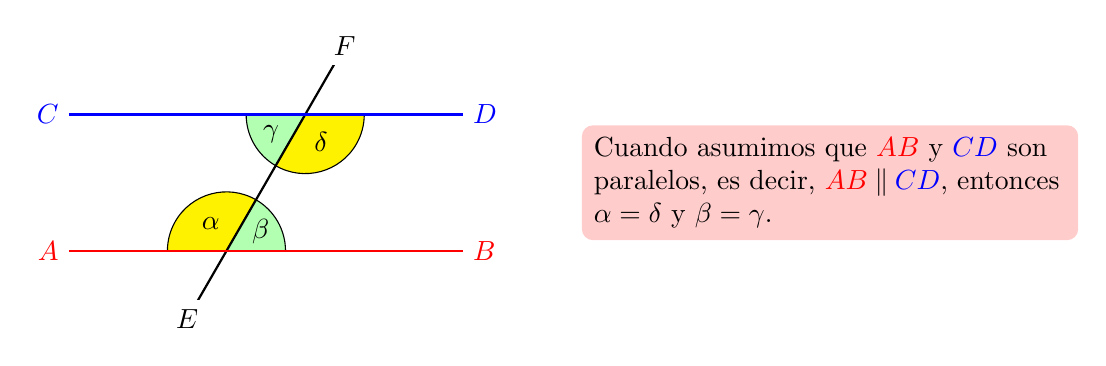
\begin{tikzpicture}
	  \draw[fill=yellow] (0,0) -- (60:.75cm) arc (60:180:.75cm);
	  \draw(120:0.4cm) node {$\alpha$};
	  \draw[fill=green!30] (0,0) -- (right:.75cm) arc (0:60:.75cm);
	  \draw(30:0.5cm) node {$\beta$};
	  \begin{scope}[shift={(60:2cm)}]
	    \draw[fill=green!30] (0,0) -- (180:.75cm) arc (180:240:.75cm);
	    \draw (30:-0.5cm) node {$\gamma$};
	    \draw[fill=yellow] (0,0) -- (240:.75cm) arc (240:360:.75cm);
	    \draw (-60:0.4cm) node {$\delta$};
	  \end{scope}
	  \begin{scope}[thick]
	    \draw  (60:-1cm) node[fill=white] {$E$} -- (60:3cm) node[fill=white] {$F$};
	    \draw[red]                   (-2,0) node[left] {$A$} -- (3,0) node[right]{$B$};
	    \draw[blue,shift={(60:2cm)}] (-3,0) node[left] {$C$} -- (2,0) node[right]{$D$};
	    \draw[shift={(60:1cm)},xshift=4cm]
	    node [right,text width=6cm,rounded corners,fill=red!20,inner sep=1ex]
	    {
	      Cuando asumimos que $\color{red}AB$ y $\color{blue}CD$ son paralelos, es decir, ${\color{red}AB} \mathbin{\|} \color{blue}CD$, entonces $\alpha = \delta$ y $\beta = \gamma$.
	    };
	  \end{scope}
	\end{tikzpicture}
\caption[Ejemplo de uso de PGF/Ti\textit{k}Z]{Ejemplo de uso de PGF/Ti\textit{k}Z, pero solo una muestra de sus capacidades.}
\label{F:tikz}
\end{figure}

Una buena cantidad de ejemplos están disponibles en \url{http://www.texample.net/tikz/} y la documentación (incluyendo un manual de uso de más de 700 páginas) está en \url{https://www.ctan.org/pkg/pgf?lang=en}.

%---------------------------------------
\subsection{Gráfico de datos y funciones con \texttt{pgfplots}}

%---------------------------------------
\subsection{Circuitos con Circuitikz}

El paquete \texttt{circuitikz} permite la creación de circuitos eléctricos y electrónicos. La Figura \ref{F:ampop} es un ejemplo.

\begin{figure}
  	\centering
		 \begin{circuitikz}[american]
		  \draw
		  % El amplificador operacional
		  (0,0) node[op amp] (opamp) {} node[] {{\tiny Amp Op}}
		  
		  % Las entradas
		  (opamp.-) node[circ] {} to[R, l_=$R_1$] ++(-2,0) node[ocirc] {} node[left] {$V_{s}$}
		  (opamp.+) -- ++(0,-0.5) node[ground] {} 
		  
		  % El lazo de realimentación
		  (opamp.-) -- ++(0,1)  to[R, l=$R_2$] ++(2,0) -| (opamp.out) {}
		  
		  % La salida
		  (opamp.out) -- ++(0.5,0) node[circ] {} to[R, l=$R_L$] ++(0,-2) to [short, i_=$I_o$] ++(0,0) node[ground] {}
		  (opamp.out) -- ++(1,0) node[ocirc] {} node[right]{$V_o$}
		  
		  ;
		\end{circuitikz}
    \caption[Amplificador inversor]{Amplificador inversor con un amplificador operacional cuya relación entrada--salida está dada por $V_o = -\frac{R_2}{R_1} V_s$.}
    \label{F:ampop}
\end{figure}

\begin{figure}
\centering
\begin{circuitikz}
\draw
	(0,0)
    	to [V, l=50~\si{\volt}] (0,2) to (0,3)
        to [R, l=$20~\si{\kilo\ohm}$] (5,3) to (5,2)
        to [vR, l=$R$] (5,0)
        to (0,0)
  	(0,2)
    	to [R, l_=$5~\si{\kilo\ohm}$] (5,2)     
;
\end{circuitikz}
\caption{Circuito básico.}
\label{F:circuitobasico}
\end{figure}

\begin{figure}
\centering
\begin{circuitikz}
\draw
	(0,0) node[ground]{}
    	to [V, l=(``Arenal'') $V_{1}$] (0,3)
        to [short] (0.5,3) node[circ]{}
   	(5.5,3)
        to [short] (5.5,4)
        to [R, l=$R_{1}$, i<=$I_{1}$] (3,4)
        to [cV, l=$v_{1}$] (0.5,4)
        to [short] (0.5,3)   
   	(6,3)
    	to [short] (5.5,3)
        to [short] (5.5,2)
        to [R, l=$R_{3}$, i<=$I_{2}$] (3,2)
        to [cV, l=$v_{3}$] (0.5,2)
        to [short] (0.5,3)
	(6,3) node[circ]{}
    	to [generic, i_=$I_{L}$, v^=$v_{L}$] (6,0) node[ground]{}
   	(6,3)
    	to [R, l=$R_{2}$, i<=$I_{3}$] (8.5,3)
        to [cV, l=$v_{2}$] (11,3)
    (11,0) node[ground]{}
        to [V, l_=$V_{2}$ (``Miravalles'')] (11,3)
;
\end{circuitikz}
\caption[Circuito de transmisión de potencia]{Circuito de transmisión de potencia por varias líneas conductoras desde centros de generación y con sistemas de ajuste de la corriente.}
\label{F:transmisionpotencia}
\end{figure}

\begin{figure}
\centering
\begin{circuitikz}
\draw 
(0,0)	to [battery, l_=$V_i$] (0,3)
		to [R, l_=$R_1$] (2.5,3)
        to [cV, l_=$A v_x$] (5,3)
        to [short] (6,3)
        to [vR, l_=$R_T$, i=$i_{R_T}$] (6,0) node[ground]{}
        to [short] (0,0)
(6,3)	to [short] (7,3)
(6,0)	to [short] (7,0)

;
\draw (2.5,3) to [open, v=$v_x$] (2.5,0);
\draw (2.5,3) node[circ]{};
\draw (2.5,0) node[circ]{};

\draw[dashed] (-0.8,-0.8) rectangle (4.8,3.8);
\draw (-0.8,-0.8) node [above right]{Fuente de corriente};

\draw (7,-0.5) rectangle (9,3.5);
\draw (8,1.5) node [align=center]{Circuito \\ de acople};

\draw 
(9,3)	to [short] (10,3)
		to [R, l_=$R_2$] (12,3)
		to [generic, l_=$Y$, v^=$v_Y$] (14,3)
(9,0)   to [short] (14,0) node[ground]{}
		to [cV, l=$A v_z$] (14,3)
(14,0)	to [short] (15.3,0)
		to [open, v>=$v_o$] (15.3,3)
		to [short] (14,3)
;
\draw (12,3)	to [open, v=$v_z$] (12,0);
\draw (12,3) node[circ]{};
\draw (12,0) node[circ]{};

\draw[dashed] (9.8,-0.8) rectangle (14.8,3.8);
\draw (9.8,-0.8) node [above right]{Amplificador};

\draw (15.3,3) node[circ]{} node[right]{$a$};
\draw (15.3,0) node[circ]{} node[right]{$b$};
\end{circuitikz}
\caption[Circuito de acondicionamiento y amplificación]{Circuito de acondicionamiento y amplificación de la señal de un sensor resistivo $R_T$, dependiente de la temperatura.}
\label{F:acondicionamiento}
\end{figure}

\begin{figure}
\centering
\begin{circuitikz}

% PNP Q1
\draw
	(0,4) 	node[pnp,rotate=90](Q1){} node[above]{$Q_1$}
;
% NPN Q2
\draw
	(0,1.5) 	node[npn,rotate=180,yscale=-1](Q2){} node[left]{$Q_2$}
;
% Op Amp
\draw
	(3,1.5) 	node[op amp,rotate=180,yscale=-1](CMP){} node[]{AMP}
;
% Resistores
\draw
	(6,4) node[circ]{} 
    	to [R, l=$R_1$] (6,2) 
    	to [R, l=$R_2$] (6,0) node[ground]{}
;
% Conectores
\draw
	(-1.5,4) 	node[ocirc]{} node[above]{$V_{IN}$} 
    		to [short] (Q1.emitter)
  	(Q1.base) to [short] (Q2.collector)
    (Q2.emitter) to [short] (0,0) node[ground]{}
    (CMP.out) to [short] (Q2.base)
    (Q1.collector) to [short] (7,4) node[ocirc]{} node[above]{$V_{OUT}$}
    (CMP.-) to [short] (6,2) node[circ]{}
    (4.5,0) node[ground]{} to [battery,l_=$V_{R}$] (4.5,1) to [short] (CMP.+) 
;
\end{circuitikz}
\caption{Regulador lineal de tensión con lazo de control.}
\label{F:reguladorlineal}
\end{figure}

\begin{figure}
\centering
\begin{circuitikz} 
\draw
	(0,0) node[op amp,yscale=-1] (opamp) {}
    (0,0) node[](){CMP}
;

\draw 
	(-4.5,2) node[rground, yscale=-1](){} 
    to [I, l_=$I$] (-4.5,1)
    to [short,-*] (-4.5,0.5)
    to [short] (-4.5,-1.8) 
;

\draw 
	(-3,2) node[rground, yscale=-1](){} 
    to [I, l_=$I$] (-3,1)
    to [short,-*] (-3,-0.5) 
    to [R, l_=$R_1$] (-3,-2.5)
    to [R, l_=$R_2$] (-3,-4.5) node[ground](){}
;

\draw 
	(-3,-2.5) to [short,*-] (-2,-2.5)
    to [cspst,] (-2,-4.5) 
    to [short] (-3,-4.5)
    (-1.8,-3.8) node[right](){SW}
;

\draw 
	(-4.5,-2.5) node[pnp](pnp){}
	(pnp.base) node[anchor=east] {\tiny{B}}
    to [short] (-5.3,-4.5) to [short,-*] (-4.5,-4.5)
    (pnp.emitter) node[anchor=east]{\tiny{E}} 
    (pnp.collector) node[anchor=east] {\tiny{C}}
    to [short] (-4.5,-4.5) to [short,-*] (-3,-4.5)
    (-4.5,-2.5) node[anchor=west] {$Q_T$}
;

\draw (opamp.-) to [short] (-3,-0.5) node[anchor=east]{$V^-$};
\draw (opamp.+) to [short] (-4.5,0.5) node[anchor=east]{$V^+$};
\draw (opamp.out) to [short] (1.5,0);
\draw[dashed] (1.5,0) -- (1.5,-3.4) -- (-1.7,-3.4);

\draw (4,0)  node[ocirc]{} node[anchor=south]{\={S}} to [full diode] (1.5,0) node[circ]{} node[anchor=south]{$V_{\mathrm{CMP}}$};

\end{circuitikz}
\caption{Circuito para protección térmica con lazo de histéresis.}
\label{F:protecciontermica}
\end{figure}

\subsection{Inserción de código fuente}
%%%%%%%%%%%%%%%%%%%%%%%%%%%%%%%%%%%%%%%

En ocasiones es necesario introducir secciones de código fuente de programación dentro de reportes. La inserción es especial, pues el compilador no debe confundir las instrucciones dentro del código con instrucciones de \LaTeX. Además, se prefiere un formato específico con resaltado de sintaxis para mejorar la legibilidad (como en los editores de código o en los IDE). Un paquete que provee soluciones para este requisito es \texttt{listings}.

Para el código fuente hecho en Matlab es posible utilizar el paquete \texttt{mcode} (adjunto como archivo a la carpeta que contiene el proyecto) que asigna a \texttt{listings} el formato apropiado, como se ve en el siguiente código:

\lstinputlisting[inputencoding=latin1]{codigo/codigoejemplo.m}

%%%%%%%%%%%%%%%%%%%%%%%%%%%%%%%%%
\section{Referencias para \LaTeX}
%%%%%%%%%%%%%%%%%%%%%%%%%%%%%%%%%

La comunidad de usuarios de \LaTeX~ es grande y colaborativa. Hay multitud de recursos en línea para aprender buenas prácticas y ``trucos'' para mejorar los documentos. Algunas de las mejores referencias son:

\begin{description}
\item[Wikibook] \url{https://en.wikibooks.org/wiki/LaTeX}
\item[Cookbook] \url{http://latex-cookbook.net/}
\item[TeXample] \url{http://texample.net/}
\item[HowtoTeX] \url{http://www.howtotex.com/}
\item[Font Catalogue] \url{http://www.tug.dk/FontCatalogue/}
\end{description}

\subsection{¿Dónde editar \LaTeX?}\label{S:programas}
%%%%%%%%%%%%%%%%%%%%%%%%%%%%%%%%%%%%%%%%%%%

\paragraph{Editores de texto ``de escritorio''}

Existen varios programas para la edición y compilación de archivos de \LaTeX. Se ha escogido Texmaker debido a que es multiplataforma (Mac, Linux, Windows) y cuenta con otras características como resaltado de sintaxis, autocompletar, corrección ortográfica, asistente para la creación de documentos, accesos rápidos a símbolos, comandos y entornos, entre otros. Se puede, claro está, editar el documento con cualquier editor y compilar, siempre y cuando se tengan los paquetes necesarios\footnote{Esta es una ventaja de ser un código estándar abierto.}.

En Windows, junto con Texmaker debe instalarse MiKTeX, que es un conjunto de paquetes, fuentes y demás necesarios para compilar el archivo.

Ambos están disponibles para descarga gratuita desde \url{http://miktex.org/} y \url{http://www.xm1math.net/texmaker/}.

Una base de datos extensiva de los paquetes de \LaTeX~ está en \url{http://www.ctan.org/}. Es especialmente útil para encontrar la documentación de los paquetes. Desde esta página se pueden descargar los paquetes, pero la mejor forma de revisar los paquetes disponibles e instalarlos fácilmente es a través del \emph{MiKTeX Package Manager}, disponible después de instalar el MiKTeX.

\paragraph{Plataformas en línea de edición para \LaTeX}

Una alternativa muy popular de años muy recientes es la edición en línea. Entre las ventajas se encuentran: almacenamiento en línea, edición colaborativa, herramientas web (bibliografías y otros), compilación simultánea, más la mayoría de las otras ventajas de los editores ``de escritorio'' como autocompletar, símbolos, etc.

Los editores más populares son:

\begin{description}
\item[Overleaf] \url{https://www.overleaf.com/}
\item[ShareLaTeX] \url{https://www.sharelatex.com/}
\item[Papeeria] \url{https://papeeria.com/}
\end{description}
% ----------------------------------------
  \chapter{Conclusiones y recomendaciones}
% ----------------------------------------
\label{C:conclusiones}

El informe debe terminarse con la enumeración de las principales conclusiones derivados del trabajo realizado.  En particular, debe verificarse el cumplimiento de los objetivos planteados para el mismo.

\section{Conclusiones}
El aporte (\emph{novedad}) hecho con el proyecto, debe destacarse.

Las conclusiones pueden enumerarse en forma suscinta como una lista, ya sea itemizada o numerada.

\section{Recomendaciones}
Con base en las trabajo realizado y las conclusiones sobre el mismo, puede ser necesario incluir una sección, o lista, de recomendaciones.  Por ejemplo, sobre la utilización de otro enfoque para resolver el problema.

% 8. APÉNDICES
\appendix
\chapter{Apéndice de ejemplo}

\lipsum[3]

\section{Una sección del apéndice}

\lipsum[4]

\subsection{Y una sub-sección}

\lipsum[5-8]

\subsection{Y otra sub-sección}

\lipsum[5-8]
\chapter{Un apéndice ejemplo con archivo anexo}

Para insertar archivos \texttt{.pdf} se utiliza el paquete \texttt{pdfpages}. Este paquete tiene opciones disponibles para la configuración del documento inserto.

Aquí hay dos ejemplos sencillos.

%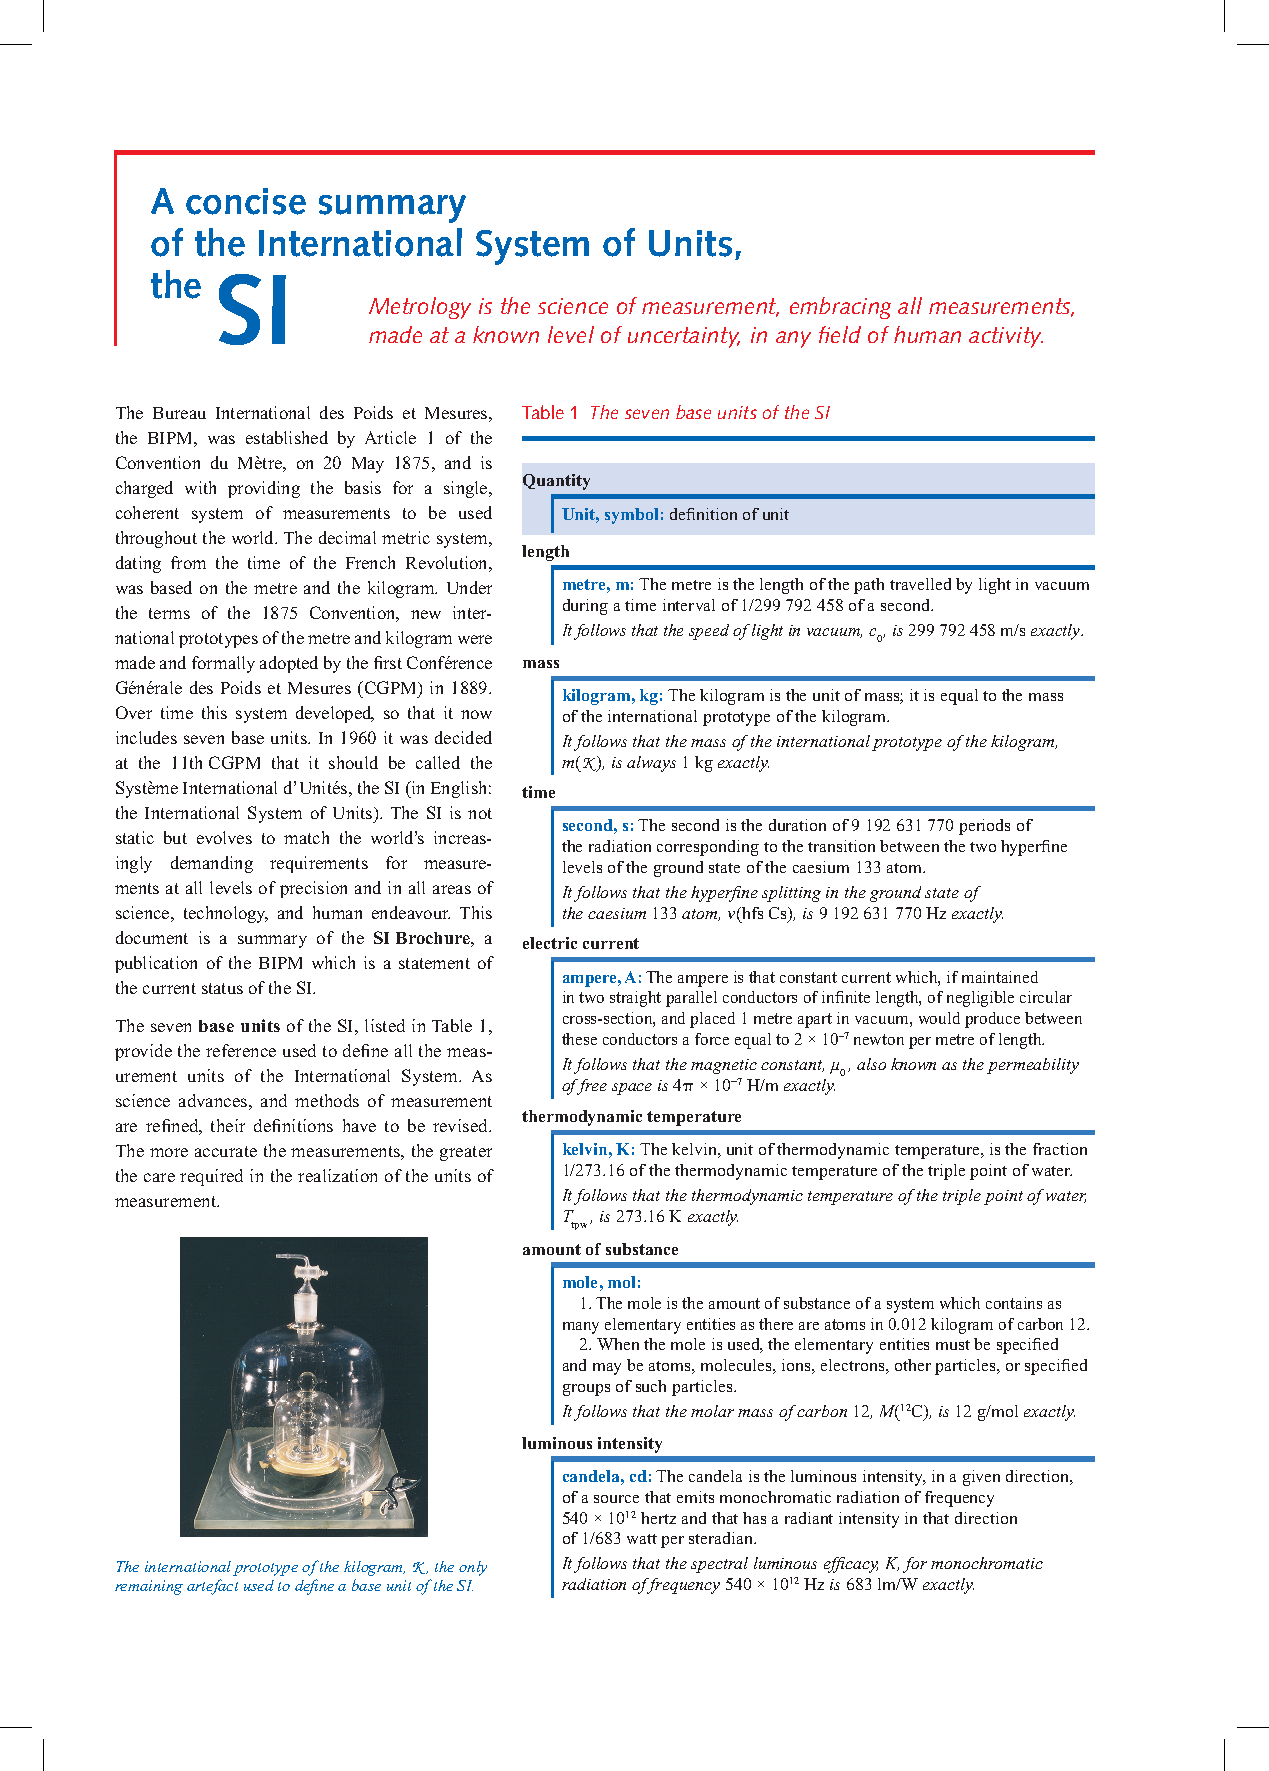
\includepdf[pages=-,nup=2x2]{apendices/SIsummary.pdf}

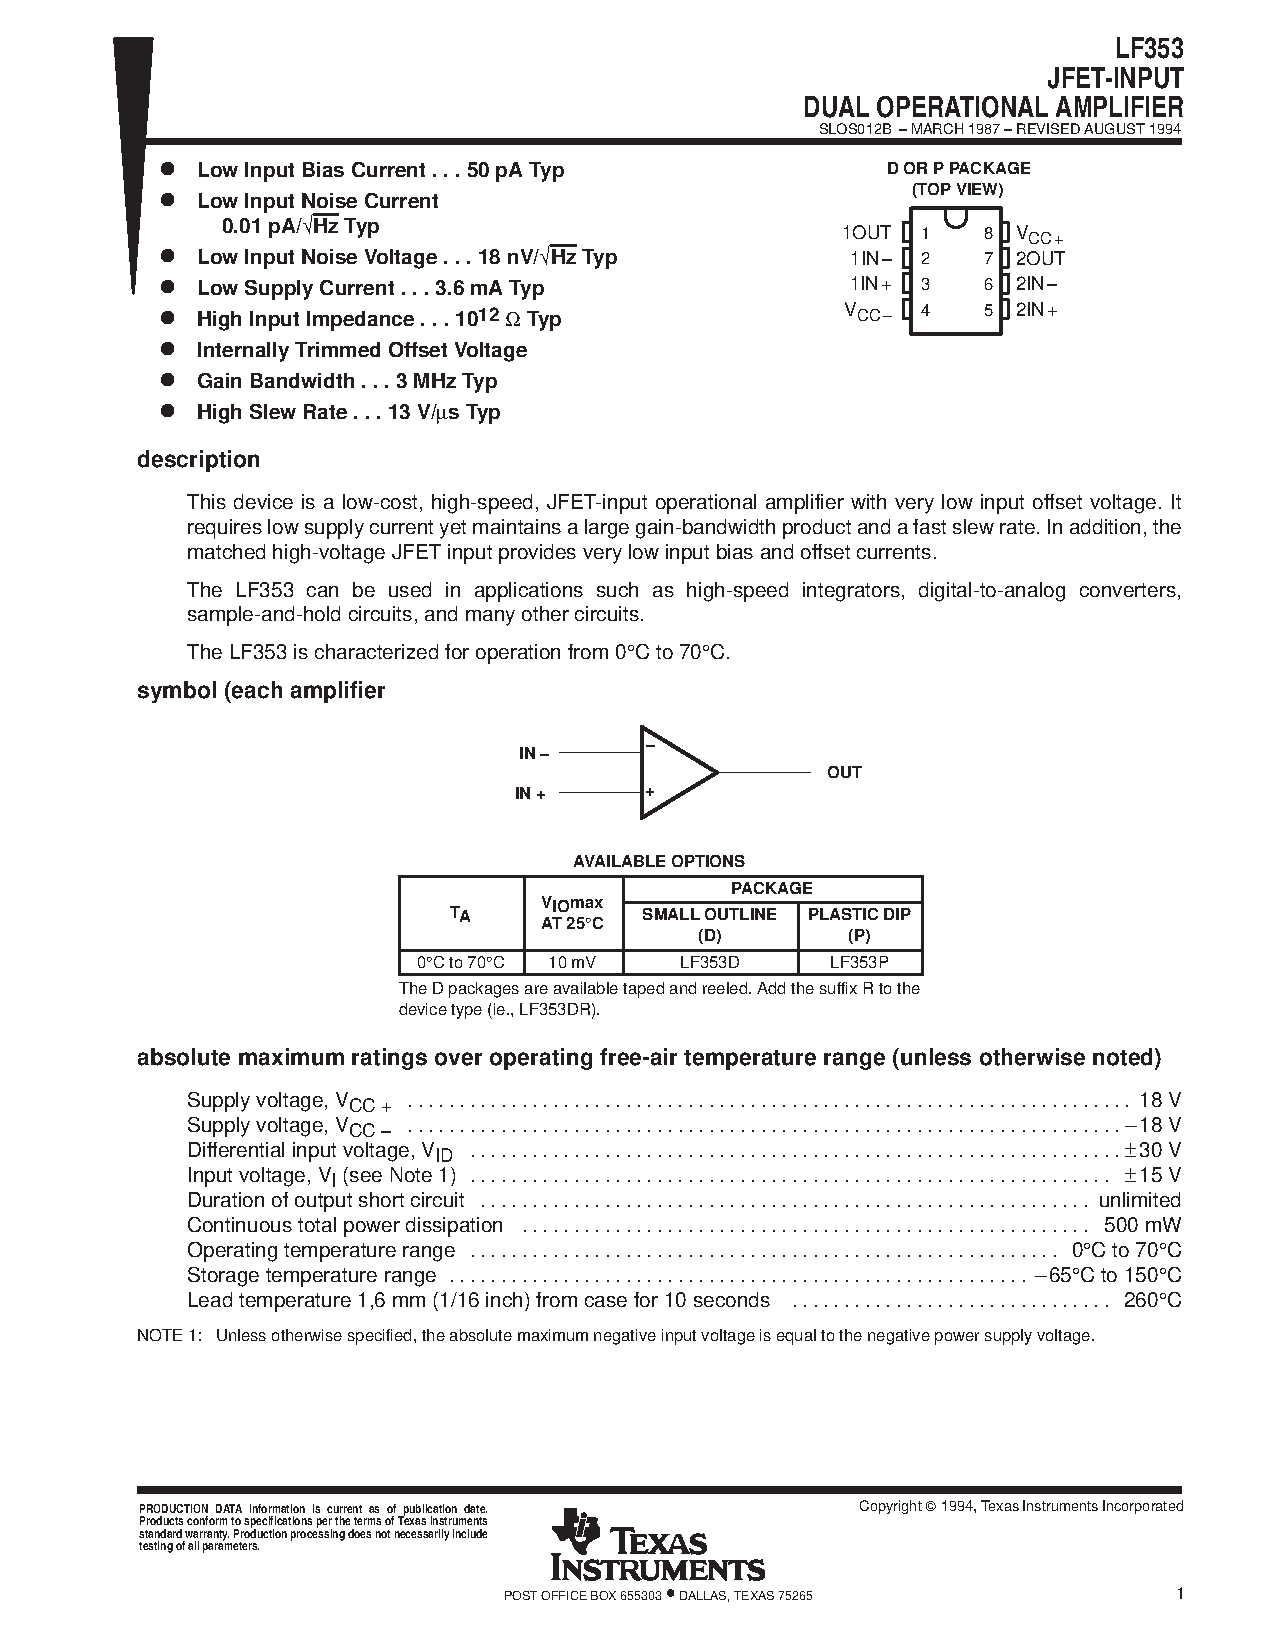
\includepdf[pages=1]{apendices/LF353.pdf}

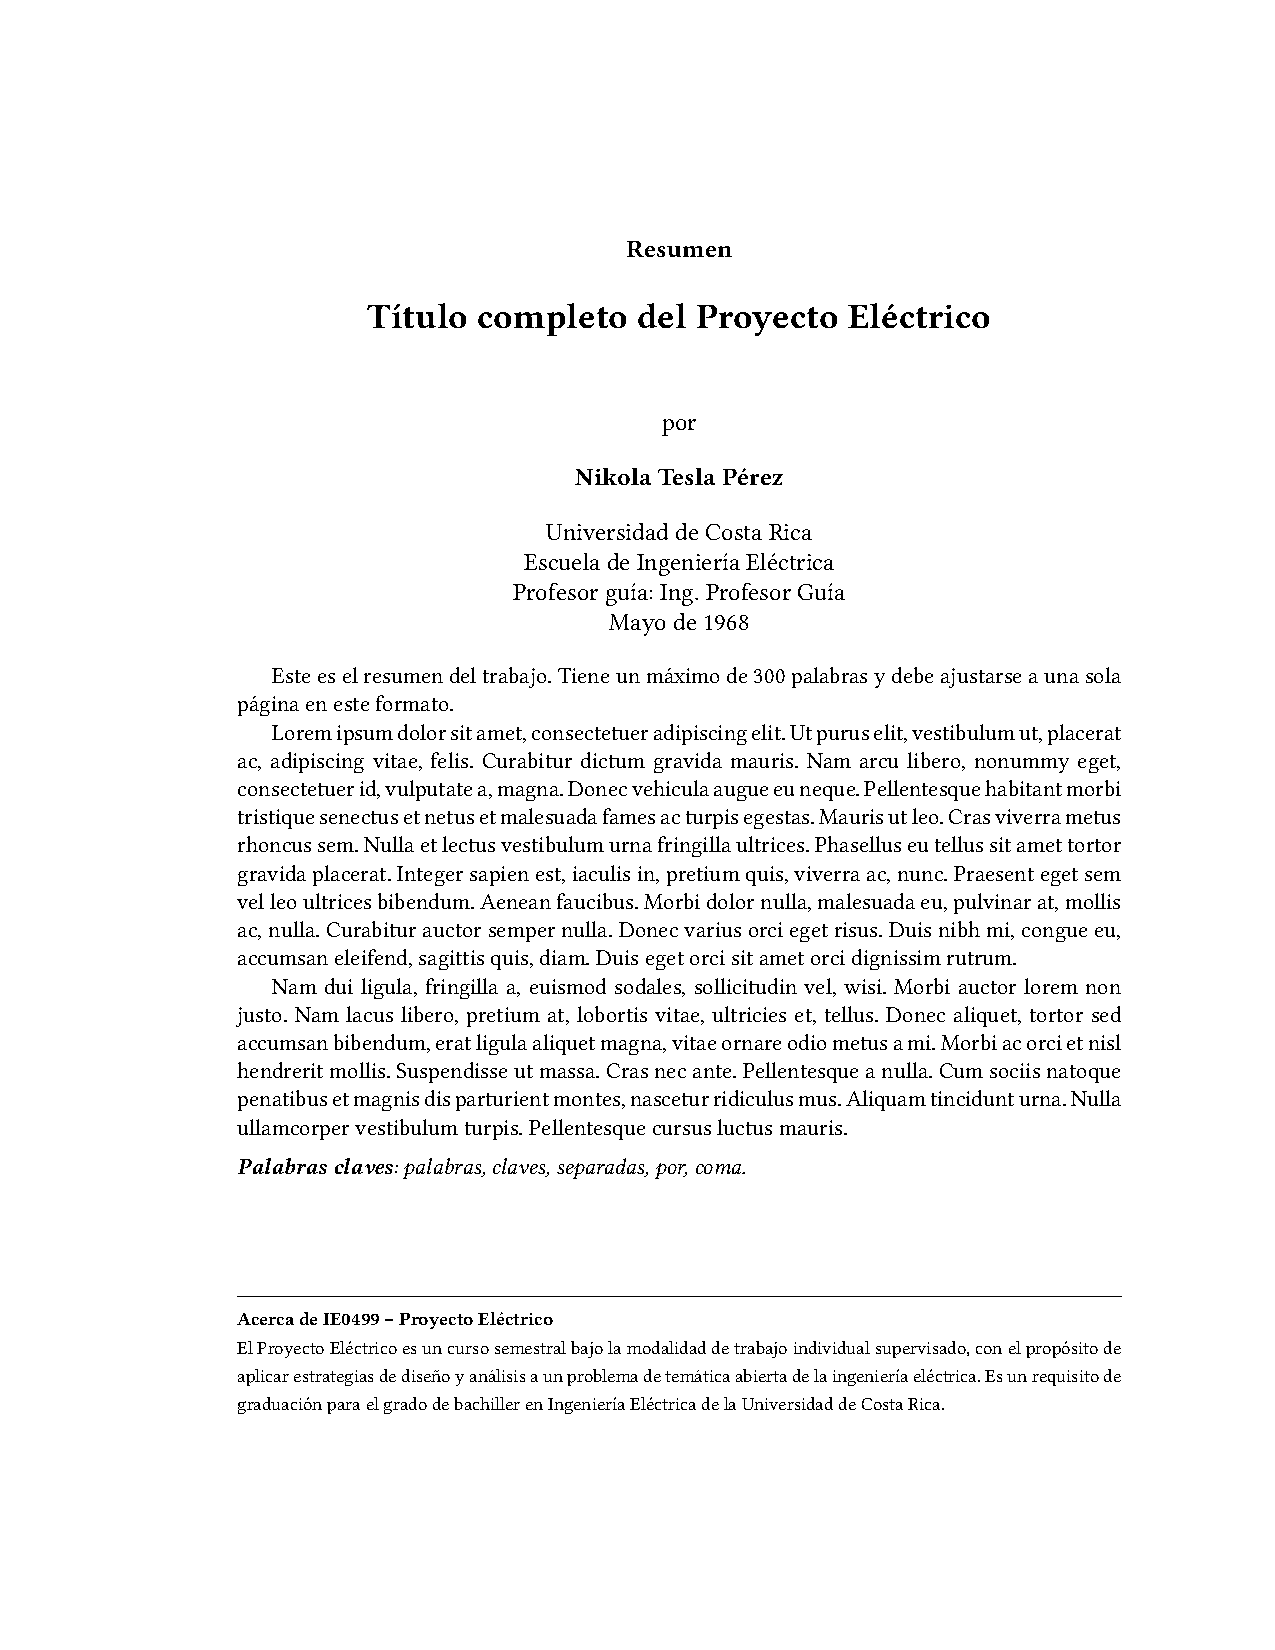
\includepdf[pages=-,scale=0.6,pagecommand={}]{apendices/Resumen.pdf}

\backmatter

% 9. BILIOGRAFÍA
\bibliographystyle{plain}
\bibliography{bibliografia/bibliografia.bib}

%%%%%%%%%%%%%%%%%%%
\end{document}
%%%%%%%%%%%%%%%%%%%